%%
%% This is file `phd_thesis.tex',
%% generated with the docstrip utility.
%%
%% The original source files were:
%%
%% dms.dtx  (with options: `TPA,gabarit')
%% Example TeX file for the documentation
%% of the jurabib package
%% Copyright (C) 1999, 2000, 2001 Jens Berger
%% See dms.ins  for the copyright details.
%% 
%%% ====================================================================
%%%  @LaTeX-file{
%%%     filename        = "dms.dtx",
%%%     author    = "Nicolas Beauchemin, Damien Rioux-Lavoie, Victor Fardel, Jonathan Godin",
%%%     copyright = "Copyright (C) 2000 , DMS
%%%                  all rights reserved.  Copying of this file is
%%%                  authorized only if either:
%%%                  (1) you make absolutely no changes to your copy,
%%%                  including name; OR
%%%                  (2) if you do make changes, you first rename it
%%%                  to some other name.",
%%%     address   = "Département de Mathématiques et de Statistique",
%%%     telephone = "514-343-6705",
%%%     FAX       = "514-343-5700",
%%%     email     = "aide@dms.umontreal.ca (Internet)",
%%%     keywords  = "latex, amslatex, ams-latex, theorem",
%%%     abstract  = " Ce fichier est un package conçu pour être
%%%                  utilisé avec la version de LaTeX2e 1995/06/01. Il
%%%                  est prévue pour la classe ``amsbook''. Il en
%%%                  modifie le format des pages, l'entête des
%%%                  sections, etc, afin d'être  conforme au modèle de
%%%                  mémoire de maîtrise de l'Université de
%%%                  Montréal. Finalement ce fichier est grandement
%%%                  inspiré du fichier amsclass.dtx.",
%%%     docstring = "The checksum field contains: CRC-16 checksum,
%%%                  word count, line count, and character count, as
%%%                  produced by Robert Solovay's checksum utility."}
%%%  ====================================================================

%% Pour voir les accents de ce fichier, assurez-vous que votre
%% éditeur de texte lise le fichier en utf-8!

%% La classe <dms> est construite au-dessus de <amsbook>, donc
%% <amsmath>, <amsfonts> et <amsthm> sont automatiquement chargés.
\documentclass[12pt,twoside,phd]{dms}
\usepackage[utf8]{inputenc} %Obligatoires
\usepackage[T1]{fontenc}    %
\usepackage{setspace}

\usepackage[backend=biber,
  style=apa,
  maxcitenames=1]{biblatex}
\addbibresource{ref.bib}


%% <lmodern> incorpore les fontes en T1, pour
%% faciliter le dépôt final. Ceci n'est pas la
%% seule option :
%%  1. Si cm-super est installé, vous pouvez enlever <lmodern>
%%     (à ce moment, la police est un peu plus fidèle
%%      au Computer Modern orginal);
%%  2. Si vous avez une police préférée, par exemple,
%%     <times> ou <euler> ou <mathpazo> (et bien d'autres),
%%     alors vous pouvez remplacer <lmodern> ci-bas.
%% Par contre, si vous faîtes face à un problème d'encapsulation
%% lors dépôt final, il se peut que la solution soit d'utiliser <lmodern>.
%% (Parfois le problème est au niveau de l'installation, donc
%%  essayez de compiler sur un autre ordinateur sur lequel vous êtes
%%  certain·e que l'installation est bonne.)
\usepackage{lmodern}
\DeclareSymbolFont{largesymbols}{OMX}{cmex}{m}{n}

% boxes
\usepackage[most]{tcolorbox}
\usepackage{lipsum}
\usepackage{xcolor}
\usepackage{tikz}

\definecolor{gre}{RGB}{101, 191, 127}
\definecolor{gree}{RGB}{7, 135, 44}


%% Il n'est pas nécessaire d'utiliser <babel>, car
%% les commandes intégrées par la classe <dms>
%% \francais et \anglais font le travail. Néanmoins,
%% certains autres packages nécessitent <babel> (comme
%% <natbib>), donc simplement enlever les % devant <babel>
%% dans ce cas. Attention! Certains packages sont sensibles
%% à l'ordre dans lequel ils sont chargés.
\francais % or
%%\anglais
%%
%%\usepackage[english,frenchb]{babel}

 % ENGLISH OPTION
 % If you call \anglais here before the \begin{document},
 % all the chater's header will be in english, even if you
 % call \francais. To change this, use
 % \entetedynamique

%% La commande \sloppy peut avoir des effets étranges sur les
%% lignes de certains paragraphes.  Dans ce cas, essayez \fussy
%% qui suppresse les effets de \sloppy.
%% (\fussy est normalement le comportement par défaut.)
%% On redéfinit \sloppy, pour tenter de réduire les comportements
%% étranges. Le seul changement apporté à la version originale
%% est la valeur de \tolerance.
\def\sloppy{%
  \tolerance 500%  %9999 dans LaTeX ordinaire, mauvaise idée.
  \emergencystretch 3em%
  \hfuzz .5pt
  \vfuzz\hfuzz}
\sloppy   %appel de \sloppy pour le document
%%\fussy  %ou \fussy

%% Packages utiles.
\usepackage{graphicx,amssymb,subfigure,icomma,makecell, flafter}
\usepackage{afterpage}
\usepackage{capt-of}
\usepackage{caption}

%% icomma       permet d'écrire les nombres décimaux en
%%                  français (p.ex. 1,23 plutôt que 1.23)
%% subfigure    simplifie l'inclusion de figures côtes-à-côtes

%% Packages parfois utiles.
%%\usepackage{dsfont,mathrsfs,color,url,verbatim,booktabs}
%% dsfont       symboles mathématiques \mathds
%% mathrsfs     plus de symboles mathématiques \mathscr
%% color        pour utiliser des couleurs (comparer avec <xcolor>)
%% url          permet l'écriture d'url
%% verbatim     pour écrire du code ou du texte tel quel
%% booktabs     plus de macros pour faire les tableaux
%%                  (voir documentation du package)

%% pour que la largeur de la légende des figures soit = \textwidth
\usepackage[labelfont=bf, width=\linewidth]{caption}

%% les 3 lignes suivante servent à l'affichage de l'index
%% dans le visionneur de pdf. <hyperref> et <bookmark>
%% devraient être les dernier package a être chargé,
%% donc chargez vos packages avant.
\usepackage{hyperref}  % Ajoute les hyperlien
\hypersetup{colorlinks=true,allcolors=black}
\usepackage{hypcap}   % Corrige la position du lien pour les images
\usepackage{bookmark} % Remédie à des petits problème
                      % de <hyperref> (important qu'il
                      % apparaisse APRÈS <hyperref>)

\makeatletter
\newcommand{\customlabel}[2]{%
   \protected@write \@auxout {}{\string \newlabel {#1}{{#2}{\thepage}{#2}{#1}{}} }%
   \hypertarget{#1}{#2}
}
\makeatother


  % Enlever les commentaires du prochaine \hypersetup et
  % le remplir avec l'information pertinente.
  % Ceci ajoute des « méta-données » au pdf.  C'est optionnel,
  % mais recommandé. Vous pouvez voir ces méta-données en
  % ouvrant un visionneur de pdf et en cherchant les propriétés
  % du pdf. (Vous pouvez aussi tapez ' pdfinfo <nom-du-pdf> '
  % dans un terminal.) Ces données sont utiles, par exemple,
  % pour augmenter les chances qu'un algorithme de recherche
  % trouve votre document sur Internet, une fois diffusé.
%%\hypersetup{
%%  pdftitle = {Titre de la thèse / du mémoire},
%%  pdfauthor = {auteur·e},
%%  pdfsubject = {Ex: Transformation de Fourier ; régressions linéaires ; ... },
%%  pdfkeywords = {Ex: mathématiques, statistiques, groupes, variables aléatoires,...}
%%}

%% Définition des environnements utiles pour un mémoire scientifique.
%% La numérotation est laissée à la discrétion de l'auteur·e. L'exemple
%% illustré ici produit « Définition x.y.z » à l'extérieur d'un article
%%   x = no. chapitre
%%   y = no. section
%%   z = no. définition
%% et « Définition x » à l'intérieur d'un article
%%   x = no. définition
%% Les numérotations des corollaires, définitions, etc.
%% se font de façon successive.
%%
%% Les macros \<type>name sont telles qu'ils suivent
%% la langue actuelle. (P.ex. si \francais est utilisé,
%% alors \begin{theo} va faire un Théorème et si \anglais
%% est utilisé, \begin{theorem} fera un Theorem.)
%%
  % Environnement à utiliser à l'extérieur des articles
\newtheorem{cor}{\corollaryname}[section]
\newtheorem{deff}[cor]{\definitionname}
\newtheorem{ex}[cor]{\examplename}
\newtheorem{lem}[cor]{\lemmaname}
\newtheorem{prop}[cor]{Proposition}
\newtheorem{rem}[cor]{\remarkname}
\newtheorem{theo}[cor]{\theoremname}

  % Environnement à utiliser à l'intérieur des articles
\newtheorem{corA}{\corollaryname}
\newtheorem{deffA}[corA]{\definitionname}
\newtheorem{exA}  [corA]{\examplename}
\newtheorem{lemA} [corA]{\lemmaname}
\newtheorem{propA}[corA]{Proposition}
\newtheorem{remA} [corA]{\remarkname}
\newtheorem{theoA}[corA]{\theoremname}
%% IMPORTANT : Il faut faire \setcounter{corA}{0}
%% au début d'un article pour recommancer à compter à 1.
%%
%% NOTE : Il peut être commode de redéfinir \the<type> pour
%% obtenir la numérotation désirée. Par exemple, pour
%% que les corollaires soit numérotés #article.#section.#sous-section,
%% on fait
%% \renewcommand\thecorA{\thepart.\thesubsection.\arabic{corA}}

%%%
%%% Si vous préférez que les corollaires, définitions, théorèmes,
%%% etc. soient numérotés séparément, utilisez plutôt un bloc de
%%% commandes de la forme :
%%%

%%\newtheorem{cor}{\corollaryname}[section]
%%\newtheorem{deff}{\definitionname}[section]
%%\newtheorem{ex}{\examplename}[section]
%%\newtheorem{lem}{\lemmaname}[section]
%%\newtheorem{prop}{Proposition}[section]
%%\newtheorem{rem}{\remarkname}[section]
%%\newtheorem{theo}{\theoremname}[section]

%%
%% Numérotation des équations par section
%% et des  tableaux et figures par chapitre.
%% Ceci peut être modifié selon les préférences de l'utilisateur.
\numberwithin{equation}{section}
\numberwithin{table}{chapter}
\numberwithin{figure}{chapter}

%%
%% Si on veut faire un index, il faut décommenter la ligne
%% suivante. Ajouter des mots à l'index avec la commande \index{mot cle} au
%% fur et à mesure dans le texte.  Compiler, puis taper la commande
%% makeindex pour creer les indexs.  Après une nouvelle compilation,
%% vous aurez votre index.
%%

%%\makeindex

%% Il est obligatoire d'écrire à double interligne
%% ou à interligne et demi. On peut soit utiliser
%% le package <setspace> ou \baselinestretch.
%% Le package a tendance a créé des grands blancs,
%% le gabarit décourage son utilisation, mais il en
%% reste à la discrétion de l'utilisateur·e.
%% \usepackage[onehalfspacing]{setspace}
 % ou
\renewcommand{\baselinestretch}{1.286} %Interligne et demi (environ 18pt (12pt+6pt) entre les lignes)

%%%%%%%%%%%%%%%%%%%%%%%%%%%%%%%%%%%%%%%%%%%%%%%%%%%%%%%%%%%%
%%%%%%%%%%%%%%%%%%%%%%%%%%%%%%%%%%%%%%%%%%%%%%%%%%%%%%%%%%%%
%%%%%%%%%%                                     %%%%%%%%%%%%%
%%%%%%%%%% D é b u t    d u    d o c u m e n t %%%%%%%%%%%%%
%%%%%%%%%%                                     %%%%%%%%%%%%%
%%%%%%%%%%%%%%%%%%%%%%%%%%%%%%%%%%%%%%%%%%%%%%%%%%%%%%%%%%%%
%%%%%%%%%%%%%%%%%%%%%%%%%%%%%%%%%%%%%%%%%%%%%%%%%%%%%%%%%%%%
\begin{document}

%%
%% Voici des options pour annoter les différentes versions de votre
%% mémoire. La commande \brouillon imprime, au bas de chacune des pages, la
%% date ainsi que l'heure de la dernière compilation de votre fichier.
%%
%%\brouillon
%%
%%
%% \version est la version de votre manuscrit
%%
\version{1}
\pagenumbering{arabic}

%%------------------------------------------------- %
%%              pages i et ii                       %
%%------------------------------------------------- %

%%%
%%% Voici les variables à définir pour les deux premières pages de votre
%%% mémoire.
%%%

\title{\centering Vers une théorie de l'entropie maximale \\ des réseaux trophiques}

\author{Francis Banville}

\copyrightyear{2024}

\department{Département de sciences biologiques}

\date{Août 2024} %Date du DÉPÔT INITIAL (ou du 2e dépôt s'il y a corrections majeures)

\sujet{sciences biologiques}
%%\orientation{orientation}%Ce champ est optionnel
%%
%% Voici les disciplines possibles (voir avec votre directeur):
%% \sujet{statistique},
%% \sujet{mathématiques}, \orientation{mathématiques appliquées},
%% \orientation{mathématiques fondamentales}
%% \orientation{mathématiques de l'ingénieur} et
%% \orientation{mathématiques appliquées}

\president{Frédérique Dubois}

\directeur{Timothée Poisot}

\codirecteur{Dominique Gravel}

\membrejury{Andrea Paz Velez}

\examinateur{Jean-Gabriel Young}   %obligatoire pour la these

%% \membresjury{Deuxième membre du jury}  % s'il y a lieu

\repdoyen{ } % (thèse seulement)

%%
%% Fin des variables à définir. La commande \maketitle créera votre
%% page titre.

%% Pour mettre bouton qui mène à la page titre
%% dans le visionneur de pdf. Peut être enlever.
\pdfbookmark[chapter]{Couverture}{PageUn}

\maketitle
\newpage
% Pour générer la deuxième page titre, il faut appeler à nouveau \maketitle
% Cette page est obligatoire.
\maketitle

\doublespacing

%%------------------------------------------------- %
%%              pages iii                           %
%%------------------------------------------------- %

% Les articles peuvent être en anglais, mais
% les autres parties du document doivent être
% en français. Il faut une permission pour
% écrire l'ensemble de la thèse en anglais.
% Consulter le guide de présentation des mémoires
% et des thèses pour de l'information plus
% précise et à jour.
\francais

\setlength{\parskip}{6pt} % pour espacement entre paragraphes

\chapter*{Résumé}

Pour bien comprendre le fonctionnement et la dynamique des écosystèmes, nous
devons développer une compréhension approfondie des réseaux d'interactions entre
espèces. Cependant, la difficulté d'échantillonner ces réseaux complique leur
étude à différentes échelles spatiales. Les modèles prédictifs peuvent pallier
ce manque de données, mais il peut parfois être difficile de choisir les
mécanismes écologiques à incorporer dans ces modèles. De plus, les sources
d'incertitude liées à ces modèles ne sont pas toujours bien identifiées, ce qui
peut nuire à notre interprétation des réseaux prédits. En reconnaissant que la
structure des réseaux trophiques est écologiquement contrainte, cette thèse met
de l'avant une méthode intrinsèquement probabiliste permettant de prédire, de
manière cohérente et non biaisée, différentes mesures des réseaux trophiques à
partir de ces contraintes. Elle jette les bases de la théorie de l'entropie
maximale des réseaux trophiques (Trophique-METE), qui permet d'inférer des
distributions de probabilité caractérisant la structure des réseaux trophiques.
Ne reposant sur aucun mécanisme écologique explicite, cette théorie prédit ces
distributions à partir du principe d'entropie maximale et d'un ensemble limité
de variables d'état, dont le choix permet de formuler différentes versions de la
théorie. 

L'article~\ref{art:article1} constitue le cadre conceptuel de la théorie. En
décrivant les sources d'incertitude des interactions entre espèces, il clarifie
la vision probabiliste des réseaux trophiques dans laquelle s'inscrit la
théorie. Je montre que cette incertitude résulte autant de notre manque de
connaissances sur les interactions entre espèces que de leur variabilité
intrinsèque dans le temps et l'espace. Je distingue deux types d'interaction
probabiliste qui diffèrent dans leurs sources d'incertitude~: les interactions
locales décrivant la probabilité qu'elles soient réalisées à un endroit et
moment particuliers, et les interactions régionales décrivant la probabilité
qu'elles soient biologiquement faisables. À l'aide d'un jeu de données
d'interactions hôtes-parasites en Europe, je montre que ces deux représentations
ont différentes propriétés statistiques, la probabilité d'interaction locale
variant dans le temps et l'espace, mais pas la probabilité d'interaction
régionale. Comprendre les propriétés des interactions probabilistes précise le
champs d'application de la théorie.

L'article~\ref{art:article2} développe les deux premières versions de la
théorie. La première utilise le nombre d'espèces et d'interactions comme
variables d'état pour prédire la distribution jointe de degrés et la matrice
d'adjacence, alors que la seconde utilise le nombre de proies et de prédateurs
par espèce pour prédire la matrice d'adjacence. Ces versions emploient deux
approches complémentaires prédisant la structure des réseaux locaux à l'aide du
principe d'entropie maximale~: l'approche analytique utilisant la méthode des
multiplicateurs de Lagrange et l'approche heuristique utilisant le recuit
simulé. Je montre que la seconde version, basée uniquement sur l'approche
heuristique, prédit bien la structure des réseaux trophiques aquatiques et
terrestres à l'échelle globale. Cependant, elle surestime leur diamètre et
niveau trophique maximal, ce qui suggère qu'une version subséquente de la
théorie contraignant la longueur des chaînes trophiques pourrait s'avérer plus
précise. Globalement, Trophique-METE facilite la prédiction des réseaux
trophiques en réduisant le nombre d'informations requises, tout en permettant
d'identifier les mécanismes écologiques importants à partir des erreurs de
prédiction.

\textbf{Mots clés} : écologie, herbivorie, incertitude, interactions entre
espèces, modélisation mathématique, parasitisme, prédation, prédiction, théorie
scientifique, variabilité locale  

%%------------------------------------------------- %
%%              pages iv                            %
%%------------------------------------------------- %

\anglais
\chapter*{Abstract}

To better understand ecosystems functioning and dynamics, we need to develop a
deep understanding of species interactions networks. However, the difficulty of
sampling these networks impedes their study at different spatial scales.
Predictive models can compensate for this lack of data, but it can be
challenging to choose which underlying ecological mechanisms to incorporate in
these models. Additionally, the sources of uncertainty associated with these
models are not always well identified, which can hinder our interpretation of
predicted networks. By recognizing that food-web structure is ecologically
constrained, this thesis introduces an intrinsically probabilistic method
generating coherent and least-biased predictions of various food-web measures
based on these constraints. It lays the groundwork for the maximum entropy
theory of food webs (Trophic-METE), which infers probability distributions
characterizing food-web structure. Without relying on explicit ecological
mechanisms, this theory predicts these distributions using the principle of
maximum entropy and a limited set of state variables, the choice of which allows
for the development of different versions of the theory.

Article~\ref{art:article1} constitutes the conceptual framework of the theory.
By describing the sources of uncertainty in species interactions, it expands the
probabilistic view of food webs that underpins the theory. I show that this
uncertainty arises both from our lack of knowledge about species interactions
and their intrinsic variability in time and space. I distinguish two types of
probabilistic interactions that differ in their uncertainty sources: local
interactions describing the probability that they occur at a specific location
and time, and regional interactions describing the probability that they are
biologically feasible. Using a dataset of host-parasite interactions in Europe,
I show that these two representations have different statistical properties,
with local interaction probabilities varying in time and space, but not regional
interaction probabilities. Understanding the properties of probabilistic
interactions helps us define the scope of the theory.

Article~\ref{art:article2} develops the first two versions of the theory. The
first version uses the number of species and interactions as state variables to
predict the joint degree distribution and the adjacency matrix, while the second
version uses the number of prey and predators per species to predict the
adjacency matrix. These versions employ two complementary approaches for
predicting the structure of local networks using the principle of maximum
entropy: the analytical approach using the method of Lagrange multipliers and
the heuristic approach using simulated annealing. I show that the second
version, based solely on the heuristic approach, accurately predicts the
structure of aquatic and terrestrial food webs at a global scale. However, it
overestimates their diameter and maximum trophic level, which suggests that a
subsequent version of the theory constraining trophic chain lengths might be
more accurate. Overall, Trophic-METE facilitates the prediction of food webs by
reducing the amount of information required while helping us identify important
ecological mechanisms from prediction errors.

\textbf{Keywords}: ecology, herbivory, local variability, mathematical modeling,
parasitism, predation, prediction, scientific theory, species interactions,
uncertainty

%%------------------------------------------------- %
%%        page v --- Table de matieres              %
%%------------------------------------------------- %

\francais
% \cleardoublepage termine la page actuel et force TeX
% a poussé les éléments flottant (fig., tables, etc.) sur
% la page (normalement TeX les garde en suspend jusqu'à ce
% qu'il trouve un endroit approprié). Avec l'option <twoside>,
% la commande s'assure que la prochaine page de texte est sur
% le recto, pour l'impression. On l'utilise ici
% pour que TeX sache que la table des matières etc. soit
% sur la page qui suit.
%% TABLE DES MATIÈRES
\cleardoublepage
\pdfbookmark[chapter]{\contentsname}{toc}  % Crée un bouton sur
% la bar de navigation

\setlength{\parskip}{0pt} % pour espacement entre paragraphes

\tableofcontents
% LISTE DES TABLES
\cleardoublepage
\phantomsection  % Crée une section invisible (utile pour les hyperliens)
\listoftables
% LISTE DES FIGURES
\cleardoublepage
\phantomsection
\listoffigures


%%%%%%%%%%%%%%%%%%%%%%%%%%%%%%%%%%%%%
%% LISTE DES SIGLES ET ABRÉVIATION %
%%%%%%%%%%%%%%%%%%%%%%%%%%%%%%%%%%%%%
%% Il est obligatoire, selon les directives de la FESP,
%% pour une thèse ou un mémoire d'avoir une liste des sigles et
%% des abréviations.  Si vous considérez que de telles listes ne seraient pas
%% pertinentes (si, par exemple, vous n'utilisez aucun sigle ou abré.), son
%% inclusion ou omission est laissé à votre discrétion.  En cas de doute,
%% parlez-en à votre directeur de recherche, le coadministrateur ou au/à la
%% bibliothécaire.
%%
%% Le gabarit inclut un exemple d'une liste « fait à la main ».  Il existe des outils
%% plus sophistiqués si vous devez inclure une multitude de sigles et abréviations.
%% Par exemple, le package <glossaries> peut faire des index élaborés.  Comme
%% son utilisation est technique, il n'y a pas d'exemple directement dans ce gabarit.
%% On invite les gens qui aurait à l'utiliser à lire la documentation officielle,
%% soit en allant sur https://www.ctan.org/, soit en tapant dans un terminal :
%%
%% texdoc glossaries
%%

\chapter*{Liste des sigles et des abréviations}
% Option de colonnes: definir \colun ou \coldeux
%%% Exemple
%%% \def\colun{\bf} % Première colonne en gras
%%% Pour numéroté les entrées, on peut faire
%%% \newcount\abbrlist
%%% \abbrlist=0
%%% \def\plusun{\global\advance\abbrlist by 1\relax}
%%% \def\colun{\plusun\the\abbrlist. }
%%\def\coldeux{\relax}
\begin{twocolumnlist}{.25\textwidth}{.62\textwidth}
  MaxEnt & Entropie maximale, de l'anglais \textit{Maximum entropy} \\
  METE & Théorie de l'entropie maximale de l'écologie, de l'anglais   
  \textit{Maximum entropy theory of ecology} \\
  SVD & Décomposition en valeurs singulières, de l'anglais  \:\:\:\:\:\:\:\:\:
  \textit{Singular value decomposition} \\
  Trophique-METE & Théorie de l'entropie maximale des réseaux trophiques, de
  l'anglais \textit{Maximum entropy theory of food webs} \\
\end{twocolumnlist}

%% L'environnement <threecolumnlist> existe aussi pour trois colonnes.

%%------------------------------------------------- %
%%              pages vi                            %
%%------------------------------------------------- %

\setlength{\parskip}{6pt} % pour espacement entre paragraphes

\chapter*{Remerciements}

Rédiger cette thèse de doctorat a été pour moi un pèlerinage intellectuel plus
grand que toutes ces longues excursions pédestres que j'ai pu faire dans ma
jeunesse. Cette promenade sur les sentiers parfois tumultueux de la recherche
scientifique n'aurait pas été possible sans le soutien indéfectible de
nombreuses personnes qui m'ont accompagné tout au long de cette aventure.

Tout d'abord, merci à mes superviseurs, Timothée Poisot et Dominique Gravel,
d'avoir été de si bons guides. Vous m'avez accueilli dans la cité des
écologistes quantitatifs et computationnels et m'avez formé pour que je devienne
l'un des vôtres. Vous m'avez aidé à préciser ma destination et m'avez montré la
route pour l'atteindre. Merci pour votre support, vos conseils et votre
bienveillance.

Merci aux autres professeur.es qui m'ont supporté dans mes travaux et rassuré
que j'allais dans la bonne direction. Merci à Allison Barner et Éric Harvey pour
m'avoir conseillé et aidé à préciser mes besoins et objectifs de recherche lors
des rencontres de mon comité-conseil. Merci à Éric Harvey et Erica Newman pour
vos questions et propositions lors de mon examen de synthèse. Un grand merci
également aux trois membres du jury qui ont accepté d'évaluer cette thèse,
Andrea Paz Velez, Frédérique Dubois et Jean-Gabriel Young. Merci à Timothée
Poisot et Dominique Gravel pour votre soutien et participation sur ces trois
comités.

Merci à mes collègues de labo et ami.es, Alexandre Fuster-Calvo, Alice Doucet
Beaupré, Andrew MacDonald, Ariane Bussières-Fournel, Benjamin Mercier, Camille
Rondeau Saint-Jean, Claire-Cécile Juhasz, Cole Brookson, Cristian Cruz
Rodriguez, Daphnée Lecours-Tessier, Dominique Caron, Emily Beasley, Eva Delmas,
Gabriel Bergeron, Gabriel Dansereau, Gracielle Higino, Kari Norman, Katherine
Hébert, Maria Isabel Arce-Plata, Mathilde Besson, Mathis Gheno, Michael Catchen,
Nerea Montes Pérez, Norma Forero-Muñoz, Philippe Desjardins-Proulx, Salomé
Bouskila, Samuel Provencher-Tardif, Steve Vissault, Tanya Strydom, Valentine
Volz, Victor Cameron, Vincent Beauregard et Willian Vieira. Vous avez été mes
compagnons de voyage, partageant avec moi différents tronçons de cette excursion
qui, sans vous, aurait été bien plus solitaire. 

Un merci spécial à Andrew MacDonald, qui m'a encouragé et accompagné dans mes
premiers pas dans la recherche scientifique. Tu as été mon mentor et seras
toujours pour moi un modèle d'écologiste attentionné, généreux et passionné. Un
autre merci spécial à Gabriel Dansereau, qui a été à mes côtés tout au long de
mon doctorat. Ton calme, ta sagesse et ton expertise m'ont permis d'avancer
lorsqu'un obstacle se dressait sur mon chemin.

Merci à l'ensemble de mes coauteurs pour nos échanges d'idées et discussions
stimulantes. Merci à Chris Brimacombe, Dominique Gravel, Gabriel Dansereau,
Gracielle Higino, Hana Mayall, Kari Norman, Michael Catchen, Penelope Blyth,
Tanya Strydom, Thomas Malpas et Timothée Poisot pour m'avoir aidé à améliorer la
qualité de cette thèse. Grâce à vous, j'ai pu avancer beaucoup plus loin que ce
que j'aurais imaginé. Merci également à mes autres coauteurs de m'avoir
accueilli dans des quêtes secondaires. Ensemble, nous avons rédigé pas moins de
11 articles scientifiques au-delà de cette thèse, dont 8 ont déjà été publiés au
moment où j'écris ces lignes. Loin d'être une distraction, ces détours m'ont
permis de me retrouver et d'élargir mes horizons. Ce fut un réel plaisir
d'explorer avec vous des sujets aussi variés que la prédiction des réseaux
écologiques, la vulgarisation scientifique et la transmission des connaissances
en programmation.

Merci à BIOS², en particulier à Andrew MacDonald, Gracielle Higino et Kim
Gauthier Schampaert, d'avoir développé une communauté de support pour les
biologistes computationnels comme moi et d'avoir organisé des ateliers et cours
d'été en statistique et programmation appliqués à l'écologie. Vous avez fait une
énorme différence dans mon parcours.

Merci à Andrew Blakney, Emmanuelle Chrétien, Morgan Botrel et Stéphanie Shousha
de m'avoir accueilli dans votre club de lecture. Nos discussions sur la
philosophie des sciences, le féminisme et le colonialisme ont changé ma vision
des sentiers académiques et ont permis de remettre le « Ph » dans mon PhD. 

Merci à Émmélie Leroux, Francis Robitaille, Julie Brémaud, Mobina Gholamhosseini
et Vincent Melancon pour avoir organisé avec moi le symposium 2023 du
département de sciences biologiques de l'Université de Montréal. Vous avez fait
d'une épreuve éprouvante l'une de mes meilleures expériences au doctorat.

Merci à Alexandre Collin de m'avoir donné l'opportunité d'enseigner une partie
de ton cours de biostatistique pendant deux ans. Cette expérience m'a donné la
piqûre pour l'enseignement des sciences, pour montrer à mon tour le chemin à la
nouvelle génération de scientifiques.

Merci à ma famille et à mes ami.es d'avoir été à mes côtés. Merci à Rebecca
Burdayron d'avoir été là pour moi lorsque je débutais tout juste cette aventure.
Un merci spécial à Léa Rancourt et Céleste Sorel de m'avoir aidé à me relever
lorsque je traversais une période plus difficile en pleine pandémie. Merci
également à mes parents, mes beaux-parents et mon frère qui, sans connaître ma
destination, m'ont encouragé et supporté tout au long de mon parcours
universitaire, qui s'est échelonné sur pas moins de 11 longues et belles années.
Vous m'avez déposé devant des sentiers nouveaux avec tout ce dont j'avais besoin
pour réussir la traversée, ayant confiance que j'allais trouver mon chemin.

Finalement, merci Sufia, ma jaan. Tu m'as accompagné dans la dernière ligne
droite de notre traversée de l'île de Montréal à pied alors qu'on ne se
connaissait à peine, et tu es toujours à mes côtés maintenant que je complète
les dernières étapes de cette odyssée doctorale. Merci pour ta positivité et tes
encouragements constants. Avec toi mon avenir après le doctorat est radieux. 

Ce travail n'aurait pas été possible sans le soutien financier de l'Institut
pour la valorisation des données (IVADO), du Programme de formation en sciences
et services de la biodiversité computationnelle (BIOS²), financé par le
Programme de formation orientée vers la nouveauté, la collaboration et
l'expérience en recherche (FONCER) du Conseil de recherches en sciences
naturelles et en génie du Canada (CRSNG), des Études supérieures et
postdoctorales (ESP) de l'Université de Montréal, du Département de sciences
biologiques de l'Université de Montréal et des fonds du laboratoire Poisot. 

\chapter*{Avant-propos}

La première moitié de mon doctorat fut marquée par la pandémie mondiale de
COVID-19, qui eut des conséquences sociales et économiques sans précédent. Un
virus respiratoire, le SRAS-CoV-2, a mis à rude épreuve les systèmes de santé
partout dans le monde, tout en nécessitant la mise en œuvre de politiques de
distanciation sociale aux conséquences psychologiques bien visibles. Maintenant
derrière nous, cette épreuve nous a collectivement fait prendre conscience de la
vulnérabilité de notre système de santé, en plus de mettre en lumière les
conséquences possibles d'un contact trop étroit avec la faune. En dépit de cela,
les activités humaines, comme la modification de l'utilisation du territoire et
le rejet de gaz à effet de serre dans l'atmosphère, n'ont pas ralenti depuis la
fin de la pandémie, même si nous savons qu'elles peuvent altérer la distribution
et la biologie des espèces hôtes de pathogènes. Rien pour atténuer son
éco-anxiété, le risque est réel de voir émerger une nouvelle crise
sanitaire causée par des changements environnementaux d'origine anthropique. 

C'est dans ce contexte que s'est développé mon intérêt pour les réseaux
écologiques. Pour mieux anticiper et nous préparer adéquatement aux changements
environnementaux à venir, que ce soit en lien avec le risque d'une future
pandémie, la sécurité alimentaire mondiale ou la pérennité d'autres services
écosystémiques, il est nécessaire de connaître la distribution des espèces et
leurs interactions. Si les interactions hôtes-parasites, comme celles entre les
chauves-souris et les bétacoronavirus, sont une préoccupation majeure en matière
de santé publique, il est crucial de préserver les interactions
plantes-pollinisateurs afin de maintenir la culture de nombreuses plantes
comestibles. De même, les interactions prédateurs-proies sont une composante clé
de la réponse des écosystèmes aux changements environnementaux puisqu'elles
déterminent les flux de matière et d'énergie. Cependant, la difficulté
d'observer les interactions entre espèces dans les milieux naturels complique
considérablement notre capacité à développer des stratégies de gestion
environnementale éclairées et à évaluer les risques qu'une nouvelle maladie
infectieuse se transmette à l'humain. Je crois que l'écologie doit s'élever au
rang d'une science prédictive pour répondre à ces enjeux.

Lors de mon doctorat, j'ai participé à plusieurs projets de recherche portant
sur la prédiction des réseaux d'interactions entre espèces à partir des données
écologiques disponibles. Dans \textcite{Strydom2021Roadmapa}, nous avons proposé une
feuille de route pour améliorer la prédiction de différents types de réseaux
écologiques dans le temps et l'espace, reconnaissant que les interactions entre
espèces peuvent varier localement. Nous avons notamment avancé que la prédiction
des réseaux écologiques à l'échelle locale est facilitée lorsque nous disposons
d'un réseau régional. Dans \textcite{Strydom2022Food}, nous avons montré qu'il est
possible de reconstituer fidèlement un tel réseau régional en transférant
l'information écologique d'un réseau analogue. Nous avons ainsi pu prédire les
interactions prédateurs-proies régionales entre les mammifères canadiens à
partir d'un réseau trophique analogue européen, qui avait été auparavant
échantillonné. Nous avons expliqué en détail la méthode utilisée d'intégration
de graphes (une méthode d'apprentissage automatique) dans
\textcite{Strydom2023Grapha}. Pour ce qui est des réseaux locaux, nous avons
développé un modèle pour prédire le nombre total d'interactions
prédateurs-proies à partir du nombre local d'espèces dans
\textcite{MacDonald2020Revisiting}. Finalement, nous avons proposé une méthode dans
\textcite{Higino2023Mismatch} pour vérifier le réalisme écologique des réseaux
trophiques locaux prédits. Bien que ces projets aient été principalement
appliqués aux interactions prédateurs-proies à cause de leur importance
historique en écologie, les méthodes présentées peuvent être appliquées à
différents types d'interactions entre espèces. 

Ma thèse s'inscrit donc dans un effort plus large visant à prédire les
interactions entre espèces à différentes échelles spatiales. J'ai approfondi et
développé dans ma thèse plusieurs des idées soulevées lors de ces projets de
recherche. Par exemple, lors d'un groupe de travail portant sur le développement
d'une méthode d'identification des sites d'échantillonnage maximisant
l'information recueillie sur les interactions entre espèces, nous avons constaté
que nous n'avions pas la même interprétation des interactions probabilistes.
Puisque nos modèles prédictifs estiment la probabilité qu'une interaction soit
réalisée, il est crucial d'avoir une interprétation claire de leurs résultats
pour pouvoir adéquatement les utiliser. La réalisation qu'il manquait une
définition précise des interactions probabilistes fut la bougie d'allumage de
l'article~\ref{art:article1}. De la même manière, c'est en travaillant sur ces
modèles prédictifs que j'ai pris connaissance que la structure des réseaux
d'interactions entre espèces était contrainte par un nombre limité de variables
écologiques. Cette constatation m'a incité à développer les bases de la théorie
de l'entropie maximale des réseaux trophiques, exposée dans
l'article~\ref{art:article2}. Cette méthode simplifie grandement la prédiction
des réseaux d'interactions entre espèces en diminuant le nombre d'information
requise. 

Mon travail est ancré dans les principes de la reproductibilité et de la science
ouverte. Je me suis engagé à partager mes données, scripts et résultats pour que
ma recherche soit plus transparente. Dans \textcite{Dansereau2020Re}, nous avons
reproduit l'article classique de \textcite{Hastings1991Chaos} sur le chaos d'une
chaîne alimentaire à trois espèces, montrant la faisabilité et l'importance d'un
tel exercice de reproduction. J'ai confiance que le lecteur ou la lectrice
désirant reproduire mes résultats de recherche trouvera cette démarche aisée.
Pour aider, nous avons rédigé un article (\cite{Banville2021Mangal}) expliquant
les librairies principales utilisées dans cette thèse. En outre, dans
\textcite{Lawlor2022Ten}, nous avons rédigé un guide pour aider les biologistes
à apprendre le langage de programmation R par eux et elles-mêmes. Les principes
généraux de ce guide peuvent également être utiles pour débuter avec le langage
de programmation Julia, qui a permis d'obtenir la majorité des résultats
présentés dans cette thèse. Enfin, je suis convaincu que notre devoir en tant
que scientifiques est de travailler ensemble et ouvertement pour relever les
défis mondiaux tels que l'adaptation aux changements climatiques, la
préservation des habitats naturels et la prévention de futures pandémies. Je
crois fermement que la compréhension des interactions entre espèces joue un rôle
crucial dans cet objectif. 

%
% Fin des pages liminaires.  À partir d'ici, les
% premières pages des chapitres ne doivent pas
% être numérotées
%
\NoChapterPageNumber
\cleardoublepage
% \pagenumbering{arabic}

% Il est recommandé que chaque article soit dans son propre .tex
% Si la bibliographie de l'article doit appaître à la fin de
% l'article (plutôt qu'à la fin de la thèse), il obligatoire que
% l'article soit dans son propre .tex
%%%%%%%%%%%%%%%%%%%%%%%%%%%%%%%%%%%%%%%%%%%%%%%%%%%%%%%%%%%%
%%%%%%%%%%%%%%%%                           %%%%%%%%%%%%%%%%%
%%%%%%%%%%%%%%%%  I N T R O D U C T I O N  %%%%%%%%%%%%%%%%%
%%%%%%%%%%%%%%%%                           %%%%%%%%%%%%%%%%%
%%%%%%%%%%%%%%%%%%%%%%%%%%%%%%%%%%%%%%%%%%%%%%%%%%%%%%%%%%%%
% %%
%% This is file `01_introduction.tex',
%% generated with the docstrip utility.
%%

% Utilisez la macro de langue appropriée.
\francais   
\doublespacing
%ou
%%\anglais
\chapter*{Introduction}


%%%%% Mise en contexte 

\section{Les réseaux d'interactions entre espèces en tant que systèmes complexes}

Les systèmes complexes sont omniprésents autour de nous. Considérons les
transactions effectuées sur les marchés financiers mondiaux
(\cite{Anderson2018Economy}), où une décision prise à Toronto peut avoir des
répercussions à Londres et à Bombay en quelques minutes seulement. Pensons
également au réseau de neurones dans notre cerveau (\cite{Sporns2011Human}), qui
orchestre des milliers de signaux électriques à chaque seconde pour créer notre
expérience subjective du monde. Ou encore, à une colonie de fourmis
(\cite{Bonabeau1999Swarm}), où chaque individu suit des règles simples, mais qui
ensemble génère des comportements complexes tels que la construction de nids et
la défense du territoire. Les systèmes complexes régissent plusieurs phénomènes
importants, mais souvent difficiles à étudier, dans notre quotidien et la
nature. 

Quel que soit leur objet d'étude, les systèmes complexes sont constitués de
nombreux éléments qui interagissent entre eux (\cite{Rind1999Complexity}). Ces
interactions impliquent des échanges directs d'information, de matière ou
d'énergie (\cite{Ladyman2013What}), donnant lieu à des propriétés émergentes de
niveau supérieur (\cite{Foote2007Mathematics}). Caractéristiques fondamentales
des systèmes complexes, ces propriétés émergentes (p. ex. un krach boursier, la
conscience humaine ou le comportement d'un superorganisme) ne sont pas
déductibles des éléments pris individuellement (\cite{Nielsen2000Emergent}). Le
désordre apparent des éléments et de leurs interactions génère donc une
structure ordonnée qui est souvent au cœur des recherches sur les systèmes
complexes. 

Pour faciliter l'étude des systèmes complexes, il est courant de les représenter
sous forme de réseaux, où les éléments forment des nœuds et les interactions,
des liens entre ces nœuds (\cite{Newman2003Structure}). Dans cette thèse, je me
suis intéressé plus particulièrement aux réseaux d'interactions entre espèces,
qui servent d'outil pour mieux comprendre les systèmes écologiques complexes.
Bien ancrée dans la science des réseaux et la théorie des graphes, l'écologie
des réseaux fournit un cadre d'analyse pour étudier le fonctionnement des
écosystèmes et leur résilience face aux changements environnementaux
(\cite{Proulx2005Network}, \cite{McCann2007Protecting}, \cite{McCann2011Food},
\cite{Rooney2012Integrating}, \cite{Valiente-Banuet2019Species}). Elle développe
des méthodes pour mesurer les interactions entre espèces (p. ex.
\cite{Jordano2016Sampling}) et analyser la structure émergente des réseaux
d'interactions (p. ex. \cite{Delmas2019Analysing}), nous permettant ainsi de
mieux comprendre les caractéristiques de ces systèmes complexes. 

Cette thèse jette les bases de la théorie de l'entropie maximale des réseaux
trophiques, qui constitue une approche novatrice en écologie des réseaux
permettant de prédire la structure émergente des réseaux complexes
d'interactions à partir d'un nombre limité d'informations écologiques. Avant
d'exposer cette théorie, il convient de décrire certains concepts clés des
réseaux d'interactions entre espèces afin de mieux comprendre la composition et
la représentation mathématique de ces systèmes écologiques complexes. Les sous-sections
suivantes traitent de la nature et des mesures des interactions entre espèces et
dressent un portrait de la structure émergente des réseaux d'interactions. Ces
descriptions permettront de mieux comprendre les fondements et champs d'application
de cette nouvelle théorie écologique.

\subsection{Qu'est-ce qu'une interaction entre espèces?} 

Une communauté biologique est composée d'espèces différentes interagissant entre
elles dans un espace donné (\cite{Stroud2015Community}). Par exemple, les
milieux forestiers tempérés du Québec sont riches en espèces animales et
végétales. À cause des changements climatiques et de la fragmentation des
habitats naturels, on y retrouve maintenant des tiques \textit{Ixodes
scapularis} infectées par la bactérie \textit{Borrelia burgdorferi}, responsable
de la maladie de Lyme (\cite{Ogden2009Emergence}, \cite{Simon2014Climate}). Les
tiques juvéniles se nourrissent sur des petits mammifères, dont la souris à
pattes blanches (\textit{Peromyscus leucopus}) qui est un réservoir compétent de
la bactérie (\cite{Donahue1987Reservoir}). Les tiques adultes, quant à elles, se
nourrissent et s'accouplent sur les cerfs de Virginie (\textit{Odocoileus
virginianus}, \cite{Lane1991Lyme}). Ces deux espèces (\textit{P. leucopus} et
\textit{O. virginianus}) s'alimentent à leur tour de glands de chêne
(\cite{McShea1993Variablea}, \cite{Elkinton1996Interactions},
\cite{Wolff1996Population}, \cite{McShea2000Influence}), ce qui peut expliquer
pourquoi l'abondance des tiques dépend de celle des glands
(\cite{Ostfeld2006Climate}). Comprendre l'écologie et l'épidémiologie de la
maladie de Lyme nécessite une compréhension approfondie des interactions entre
espèces au sein des communautés où la tique \textit{I. scapularis} est présente.
Plus généralement, les interactions au sein d'une communauté biologique peuvent
être représentées à différents niveaux d'organisation (p. ex. interactions entre
individus ou espèces), décrire une variété de processus écologiques (p. ex.
interactions hôtes-parasites ou plantes-herbivores) et couvrir différentes
échelles spatiales (local ou régional).

\subsubsection{Une interaction entre individus représentée à l'échelle de l'espèce} 

Bien que les interactions se produisent biologiquement entre des
individus, elles peuvent être représentées à des niveaux d'organisation
supérieures (p. ex. au niveau de l'espèce). Les individus sont à la base des
interactions écologiques puisque ce sont eux qui effectuent les échanges
d'information, de matière ou d'énergie. Par exemple, c'est du sang d'un cerf de
Virginie particulier que s'alimentera une tique adulte. Il va sans dire que les
réseaux d'interactions entre individus sont difficiles à échantillonner, le peu
de données disponibles sur les interactions entre individus étant biaisées en
faveur d'organismes plus simples à observer (\cite{Guimaraes2020Structure}).
Pour cette raison, les interactions entre individus sont le plus souvent
groupées en des niveaux d'organisation supérieures, connectant ainsi différentes
populations, espèces ou clades entre eux (\cite{Elton1927Animal}). Les réseaux
d'interactions entre espèces, qui lient deux espèces lorsque certains de leurs
individus interagissent, ne capturent donc qu'une partie de la complexité d'un
écosystème. Ils constituent malgré tout une représentation adéquate du rôle
écologique des espèces (\cite{Delmas2019Analysing}) et des propriétés émergentes
des écosystèmes (\cite{Loreau2010Populations}, \cite{McCann2011Food},
\cite{Bascompte2013Mutualistic}, \cite{Gonzalez2020Scalingup}), tout en formant
la plupart des réseaux d'interactions échantillonnés
(\cite{Guimaraes2020Structure}). Il n'existe pas de niveau d'organisation
approprié par défaut, celui-ci dépendant de la question posée
(\cite{Niquil2020Shifting}) et des données disponibles.

\subsubsection{Une interaction pouvant décrire différents processus écologiques} 

Les interactions entre espèces peuvent avoir des effets positifs, négatifs ou
neutres sur les organismes impliqués, en fonction du type d'interaction. Les
interactions antagonistes, telles que les interactions hôtes-parasites,
prédateurs-proies et plantes-herbivores, profitent à une espèce au détriment de
l'autre. Les interactions hôtes-parasites procurent un habitat et une source
d'alimentation au parasite au prix du \textit{fitness} de l'hôte, alors que les
interactions prédateurs-proies et plantes-herbivores transfèrent l'énergie de la
ressource vers le consommateur, entraînant généralement la mort de la proie,
mais pas nécessairement celle de la plante. Les interactions mutualistes, telles
que les interactions plantes-pollinisateurs, profitent au contraire aux deux
espèces. Le pollinisateur se nourrit du nectar de la plante, qui en retour en
profite pour disperser son pollen à des fins de reproduction. Selon le niveau de
complexité représenté, les réseaux d'interactions entre espèces peuvent être
composés d'un seul type d'interaction (p. ex. les réseaux trophiques composés
exclusivement d'interactions trophiques prédateurs-proies et plantes-herbivores)
ou de plusieurs (p. ex. les réseaux multicouches composés d'interactions
antagonistes et mutualistes, \cite{Pilosof2017Multilayer}).

Les interactions prédateurs-proies et plantes-herbivores ont une importance
particulière et historique en écologie. Les réseaux trophiques ont été
introduits il y a près d'un siècle, lorsque Charles Sutherland Elton (1900-1991)
a développé les concepts de chaînes et de niveaux trophiques
(\cite{Elton1927Animal}, \cite{Elton1958Ecology}). Plusieurs publications
marquantes en écologie, comme celles de \cite{May1972Will} sur la stabilité des
écosystèmes complexes et de \cite{Lotka1925Elements} et
\cite{Volterra1927Fluctuations} sur la dynamique des populations animales,
portent sur les interactions trophiques. Les interactions prédateurs-proies et
plantes-herbivores déterminent les flux de matière et d'énergie au sein des
écosystèmes. Elles nous permettent de mieux comprendre des phénomènes tels que
la régulation de la productivité primaire par cascade trophique
(\cite{Carpenter1987Regulation}), la stabilité des écosystèmes face à
l'extirpation d'espèces (\cite{Dunne2002Network}, \cite{Srinivasan2007Response},
\cite{Staniczenko2010Structural}) et la capacité des espèces à migrer et
s'adapter aux changements climatiques (\cite{Tylianakis2008Global},
\cite{Gilman2010Framework}) et à la perte d'habitats naturels
(\cite{Evans2013Robustness}). De plus, les données disponibles sur les réseaux
trophiques couvrent une diversité d'habitats à l'échelle mondiale
(\cite{Poisot2021Global}), ce qui nous permet de tester une variété de modèles
et d'hypothèses écologiques sur ces interactions. C'est pourquoi les
interactions trophiques occupent une place centrale dans cette thèse.

\subsubsection{Une interaction réalisée localement mais cataloguée régionalement} 

Cette thèse distingue les interactions réalisées à l'échelle locale de celles
cataloguées à l'échelle régionale. Les réseaux locaux
(\cite{Poisot2012Dissimilarity}) sont constitués d'interactions observées ou
réalisées à un endroit et moment particuliers. Ce sont eux qui décrivent les
échanges directs d'information, de matière ou d'énergie ayant lieu à l'échelle
locale. Deux espèces interagissent localement si leurs abondances (nombres
d'individus) sont suffisamment élevées pour qu'elles puissent se rencontrer
(\cite{Canard2012Emergence}, \cite{Canard2014Empirical}) et que leurs traits
(caractéristiques biologiques telles que la taille corporelle) supportent une
interaction lorsqu'elles se rencontrent (\cite{Bolnick2011Why},
\cite{Gravel2013Inferring}, \cite{Stouffer2011Role}). Par exemple, les habitudes
alimentaires du cerf de Virginie varient localement selon la disponibilité
saisonnière en nourriture (\cite{Short1975Nutrition}) et sa masse corporelle
(\cite{Luna2013Influence}). Les conditions environnementales, comme la
température (\cite{Angilletta2004Temperature}), les précipitations
(\cite{Woodward2012Climate}) et l'utilisation du territoire
(\cite{Tylianakis2007Habitat}), influent également sur la réalisation des
interactions à l'échelle locale. Ces trois facteurs (abondances, traits et
conditions environnementales) contribuent à la variation spatiale et temporelle
des interactions locales (\cite{Poisot2015Species}). 

Les réseaux régionaux (ou \textit{metaweb}, \cite{Pascual2006Ecological}), quant
à eux, sont constitués d'interactions potentielles, c'est-à-dire d'interactions
biologiquement ou écologiquement faisables sans nécessairement être réalisées
localement. Par exemple, les interactions trophiques régionales du cerf de
Virginie incluent l'ensemble des plantes et champignons dont il peut se nourrir
dans différents contextes. Une interaction régionale indique si deux espèces
possèdent des traits leur permettant d'interagir dans des conditions idéales.
Les réseaux régionaux sont donc un catalogue de l'ensemble des interactions
observées (p. ex. \cite{Maiorano2020Tetraeu}) ou prédites (p. ex.
\cite{Strydom2022Food}) entre un groupe d'espèces données. Les réseaux locaux,
étant constitués d'un sous-ensemble des espèces et de leurs interactions
régionales, sont des sous-réseaux du \textit{metaweb}
(\cite{Saravia2022Ecological}). Contrairement aux réseaux locaux, les réseaux
régionaux ne varient pas spatialement ni temporellement puisqu'ils incluent
l'ensemble des interactions locales entre un groupe d'espèces. 

\subsection{Comment mesurer une interaction entre espèces?} 

Construire un réseau demande de faire des choix méthodologiques concernant les
interactions entre espèces, choix qui impacteront notre interprétation des
propriétés émergentes du réseau. Étant donné le nombre élevé d'organismes et la
diversité de leurs interactions, il est souvent nécessaire d'opter pour une
représentation simplifiée des interactions au sein d'une communauté biologique.
Cette représentation simplifiée doit contenir les informations écologiques
pertinentes au sujet d'étude, dans les limites de ce qui peut être observé. 
Ces décisions dépendent autant des objectifs de recherche que des données
disponibles.

\subsubsection{Évaluer la présence ou la valeur d'une interaction} 

\subsubsection{Évaluer l'incertitude d'une interaction} 


\subsection{Quelle est la structure émergente d'un réseau d'interactions entre espèces?} 

\subsubsection{Une structure représentée par des valeurs uniques} 

\subsubsection{Une structure représentée par des distributions} 


%%%%% La théorie de l'entropie maximale des réseaux trophiques

\section{Vers une théorie de l'entropie maximale des réseaux trophiques}

\subsection{Pourquoi avons-nous besoin d'une théorie des réseaux trophiques?} 

\subsection{Quels sont les fondements de la théorie?} 

\subsection{Que permet-elle de prédire?} 

\subsection{Quel est son champ d'application?} 

J'ai testé la théorie de l'entropie maximale des réseaux trophiques sur des
réseaux d'interactions entre espèces. Cependant, elle peut être adaptée à
d'autres niveaux d'organisation taxonomique en sélectionnant les informations
écologiques (entrées du modèle) et mesures prédites (sorties du modèle)
conformément au niveau d'organisation choisi. Dans cette thèse, je propose
également une façon d'étendre la théorie pour qu'elle puisse prédire
\textit{simultanément} les propriétés des réseaux d'interactions entre individus
et espèces. À défaut d'avoir développé une telle théorie élargie, cette thèse
explore comment différents types d'interactions écologiques varient selon le
niveau d'organisation taxonomique, alimentant une réflexion sur le champ
d'application de la théorie au-delà des interactions entre espèces. 

J'ai formulé les principes de base de la théorie de l'entropie maximale des
réseaux trophiques autour des interactions prédateurs-proies et
plantes-herbivores. Néanmoins, la théorie de l'entropie maximale des réseaux
trophiques peut être adaptée et testée sur d'autres types d'interactions qui
impliquent un échange direct d'information, de matière ou d'énergie (comme les
interactions hôtes-parasites ou plantes-pollinisateurs).

Cette distinction entre réseaux locaux et régionaux revêt d'une grande
importance dans l'élaboration de la théorie de l'entropie maximale des réseaux
trophiques, celle-ci étant mieux adaptée aux réseaux locaux. En effet, cette
théorie trouve son fondement dans la complexité des écosystèmes locaux. Les
écosystèmes complexes sont constitués, par définition, d'interactions impliquant
un échange direct d'information, de matière ou d'énergie
(\cite{Ladyman2013What}), ce qui se produit à l'échelle locale. Les réseaux
régionaux décrivent plutôt le potentiel que de tels échanges aient lieu, sans
nécessairement être réalisés. De plus, la variabilité des interactions locales
introduit une incertitude qui est non réductible (c.-à-d. qui ne diminue pas
avec davantage de données). Cela a pour conséquence de diminuer la prédictibilité des
interactions locales, rendant possiblement les réseaux locaux plus complexes. La
théorie de l'entropie maximale des réseaux trophiques vise précisément à
identifier la structure la plus complexe possible des réseaux locaux, dans la
limite de contraintes écologiques. Un chapitre complet de cette thèse est dédié
aux caractéristiques et sources d'incertitude des réseaux locaux et régionaux.


%%%%% Objectifs 

\section{Objectifs généraux de la thèse} 


%%%%% Chapitres

\section{Organisation de la thèse}

\subsection{Chapitre 1: Décrypter les réseaux d'interactions probabilistes} 

\subsection{Chapitre 2: Des modèles d'entropie maximale prédisant la structure des réseaux trophiques} 

\endinput
%%
%% End of file `01_introduction.tex'.


%%%%%%%%%%%%%%%%%%%%%%%%%%%%%%%%%%%%%%%%%%%%%%%%%%%%%%%%%%%%
%%%%%%%%%%%%%%%%%%%%                   %%%%%%%%%%%%%%%%%%%%%
%%%%%%%%%%%%%%%%%%%%  A R T I C L E 1  %%%%%%%%%%%%%%%%%%%%%
%%%%%%%%%%%%%%%%%%%%                   %%%%%%%%%%%%%%%%%%%%%
%%%%%%%%%%%%%%%%%%%%%%%%%%%%%%%%%%%%%%%%%%%%%%%%%%%%%%%%%%%%
% %%
%% This is file `02_article1.tex',
%% generated with the docstrip utility.
%%
%% The original source files were:
%%
%% dms.dtx  (with options: `article')
%% Example TeX file for the documentation
%% of the jurabib package
%% Copyright (C) 1999, 2000, 2001 Jens Berger
%% See dms.ins  for the copyright details.
%% 
%%% ====================================================================
%%%  @LaTeX-file{
%%%     filename        = "dms.dtx",
%%%     author    = "Nicolas Beauchemin, Damien Rioux-Lavoie, Victor Fardel, Jonathan Godin",
%%%     copyright = "Copyright (C) 2000 , DMS
%%%                  all rights reserved.  Copying of this file is
%%%                  authorized only if either:
%%%                  (1) you make absolutely no changes to your copy,
%%%                  including name; OR
%%%                  (2) if you do make changes, you first rename it
%%%                  to some other name.",
%%%     address   = "Département de Mathématiques et de Statistique",
%%%     telephone = "514-343-6705",
%%%     FAX       = "514-343-5700",
%%%     email     = "aide@dms.umontreal.ca (Internet)",
%%%     keywords  = "latex, amslatex, ams-latex, theorem",
%%%     abstract  = " Ce fichier est un package conçu pour être
%%%                  utilisé avec la version de LaTeX2e 1995/06/01. Il
%%%                  est prévue pour la classe ``amsbook''. Il en
%%%                  modifie le format des pages, l'entête des
%%%                  sections, etc, afin d'être  conforme au modèle de
%%%                  mémoire de maîtrise de l'Université de
%%%                  Montréal. Finalement ce fichier est grandement
%%%                  inspiré du fichier amsclass.dtx.",
%%%     docstring = "The checksum field contains: CRC-16 checksum,
%%%                  word count, line count, and character count, as
%%%                  produced by Robert Solovay's checksum utility."}
%%%  ====================================================================


%% To change chapter header dynamically from french to english, use
%%\entetedynamique
\setcounter{corA}{0} % Pour recommancer à compter les def,
                     % theo, etc. à partir de 1
 % Pour écrire un article en français
\francais
 % Pour écrire un article en anglais
%%\anglais
%% NOTE: La plupart des macros ont un nom en anglais.
%% P.ex. \adresse et \address fonctionnent et sont équivalents.
%% \revue=\journal
%% \auteur=\author
%% \titre=\title

%% Les contributions apparaîtront habituellement après
%% \maketitle (voir un peu plus bas). Selon les goûts, il est
%% possible de mettre les contributions
%% avant la page titre de l'article, simplement en les écrivant
%% directement ici. Par exemple :
 % \cleardoublepage
 % \pdfbookmark[chapter]{Contributions}{contrib1} % Remplacer par contrib2 pour l'article 2 etc.
 % {\bfseries\Large\noindent Contributions de <mon nom> et rôle joué par les coauteurs}
 % J'ai contribué en...
 %
 % Le rôle des coauteurs a été de...

%% Nom de la revue de publication
\revue{Une revue}
\article{Titre de l'article}\label{Chapter1}
%% On peut se référer aux numéros de chapitre ou d'article comme suit.
%% Si on fait
%% \label{chap:article1},
%% alors \ref{chap:article1} donnera le numéro du chapitre. On peut ensuite faire
%% \labelart{art:article1}
%% et alors \ref{art:article1} donnera le numéro d'article.
%% Par exemple, si cette article est le premier article et le deuxième chapitre,
%% alors si on écrit
%% Voir le chapitre~\ref{chap:article1} (l'article~\ref{art:article1}).
%% deviendra
%% Voir le chapitre 2 (l'article 1).
%% Si on veut écrire « premier article » au lieu « article 1 », on peut
%% simplement faire
%% \ordinal{\ref{art:article1}}~article  % devient première article
%% ou
%% \Ordinal{\ref{art:article1}}~article  % devient Première article (avec la majuscule)
%% Si on est en mode \anglais, \ordinal écrire first, second,...

 % Contribution(s) peronnelle(s) à l'article et rôle joué par tous les coauteur·e·s
 %
 % Nécessaire seulement lorsque vous n'êtes pas seul·e auteur·e.
 % Les contributions peuvent apparaître ailleur dans la thèse.
 % Si \contributions est laissé vide (p.ex. si vous effacez
 % celui ci-bas), aucune contributions ne seront générées sur
 % la page titre de l'article. Vous pouvez alors mettre un
 % \newpage si vous souhaitez que les résumé et abstract soient
 % la page suivante.
 %
 % REMARQUE : À peu près toutes les constructions \LaTeX\ sont permises
 % dans les contributions.
 %
 % La commande admet une option [<entête>]
\contributions%[Mes contributions et le rôle des coauteurs]
{
J'ai fait telle chose à l'article. J'ai rédigé telle partie
etc.

  % Exemple avec un <itemize>
  %  \begin{itemize}
  %      \item Calcul de telle chose;
  %      \item Vérification de telle équation;
  %      \item Idée pour telle définition;
  %      \item Démonstration de tel théorème.
  %  \end{itemize}

    Le coauteur1 a suggéré telle chose.

    Le coauteur2 a fait telle calcul.\\[1cm]
}

%%% INFORMATIONS POUR LA PAGE TITRE
 % Premier auteur·e et adresse
\auteur{Hima Ginère}
\adresse{1252i rue complexe\\ Université du plan complexe}
 % Deuxième auteur·e et adresse (si différente de la première)
%%\auteur{Hana Lietick}
%%\adresse{4242 rue imaginaire\\ Universität von der gau\ss sche Zahlenebene}
%%
%% et ainsi de suite pour les autres auteurs

\maketitle

\begin{resume}{Mots clés}
  Le résumé en français.
\end{resume}

\begin{abstract}{Key words}
  The english abstract.
\end{abstract}

\section{Introduction}
%%
%% Le reste de l'article...
%%

Exemple de citation~: Consultez le \LaTeX\ companien
de Mittelbach {\it et al\/}~\cite{exemple}.

 % Pour générer la bibliographie à la fin
 % de l'article, utiliser la commande de la
 % classe <dms> \sectionbibliography{<nom du .bib>}.
 % Il y a aussi la possibilité d'utiliser le package
 % <chapterbib>, auquel cas on utilise simplement
 % \bibliography normalement.
 %
 % IMPORTANT : Dans tous les cas, il faut faire
 %    pdflatex these
 %    bibtex chapitre1
 %    bibtex chapitre2
 %    .
 %    .
 %    .
 %    bibtex chapitreN
 %    pdflatex these
 %    pdflatex these
 %
 % où <these> est le nom du .tex principal
 % (qui contient le \documentclass).
 % bibtex a besoin du .aux de chapitre1 et
 % non du .tex. Il est parfois nécessaire
 % d'effacer le .aux et de recommencer la
 % compilation du début.
%%\bibliographystyle{amsplain} % style plain anglais ou
%% \bibliographystyle{amsplain-french} % style plain francais
%%\bibliographystyle{<style>} % autre
%% \sectionbibliography{ref.bib} %Donner le nom du .bib

\endinput
%%
%% End of file `02_article1.tex'.


%%%%%%%%%%%%%%%%%%%%%%%%%%%%%%%%%%%%%%%%%%%%%%%%%%%%%%%%%%%%
%%%%%%%%%%%%%%%%%%%%                   %%%%%%%%%%%%%%%%%%%%%
%%%%%%%%%%%%%%%%%%%%  A R T I C L E 2  %%%%%%%%%%%%%%%%%%%%%
%%%%%%%%%%%%%%%%%%%%                   %%%%%%%%%%%%%%%%%%%%%
%%%%%%%%%%%%%%%%%%%%%%%%%%%%%%%%%%%%%%%%%%%%%%%%%%%%%%%%%%%%
% %%
%% This is file `03_article2.tex',
%% generated with the docstrip utility.
%%
%% The original source files were:
%%
%% dms.dtx  (with options: `article')
 
%% To change chapter header dynamically from french to english, use
\entetedynamique
\setcounter{corA}{0} % Pour recommancer à compter les def,
                     % theo, etc. à partir de 1

\setcounter{figure}{0}
\renewcommand{\thefigure}{\arabic{chapter}.\arabic{figure}}

 % Pour écrire un article en français
\francais
 % Pour écrire un article en anglais
%% \anglais
%% NOTE: La plupart des macros ont un nom en anglais.
%% P.ex. \adresse et \address fonctionnent et sont équivalents.
%% \revue=\journal
%% \auteur=\author
%% \titre=\title

%% Les contributions apparaîtront habituellement après
%% \maketitle (voir un peu plus bas). Selon les goûts, il est
%% possible de mettre les contributions
%% avant la page titre de l'article, simplement en les écrivant
%% directement ici. Par exemple :
 % \cleardoublepage
 % \pdfbookmark[chapter]{Contributions}{contrib1} % Remplacer par contrib2 pour l'article 2 etc.
 % {\bfseries\Large\noindent Contributions de <mon nom> et rôle joué par les coauteurs}
 % J'ai contribué en...
 %
 % Le rôle des coauteurs a été de...

%% Nom de la revue de publication
\revue{publiée dans PLOS Computational Biology et est accessible via le lien suivant~: \url{https://doi.org/10.1371/journal.pcbi.1011458}}
\article{What constrains food webs? A maximum entropy framework for predicting their structure with minimal biases}\labelart{art:article2}
%% On peut se référer aux numéros de chapitre ou d'article comme suit.
%% Si on fait
%% \label{chap:article1},
%% alors \ref{chap:article1} donnera le numéro du chapitre. On peut ensuite faire
%% \labelart{art:article1}
%% et alors \ref{art:article1} donnera le numéro d'article.
%% Par exemple, si cette article est le premier article et le deuxième chapitre,
%% alors si on écrit
%% Voir le chapitre~\ref{chap:article1} (l'article~\ref{art:article1}).
%% deviendra
%% Voir le chapitre 2 (l'article 1).
%% Si on veut écrire « premier article » au lieu « article 1 », on peut
%% simplement faire
%% \ordinal{\ref{art:article1}}~article  % devient première article
%% ou
%% \Ordinal{\ref{art:article1}}~article  % devient Première article (avec la majuscule)
%% Si on est en mode \anglais, \ordinal écrire first, second,...

 % Contribution(s) personnelle(s) à l'article et rôle joué par tous les coauteur·e·s
 %
 % Nécessaire seulement lorsque vous n'êtes pas seul·e auteur·e.
 % Les contributions peuvent apparaître ailleur dans la thèse.
 % Si \contributions est laissé vide (p.ex. si vous effacez
 % celui ci-bas), aucune contributions ne seront générées sur
 % la page titre de l'article. Vous pouvez alors mettre un
 % \newpage si vous souhaitez que les résumé et abstract soient
 % la page suivante.
 %
 % REMARQUE : À peu près toutes les constructions \LaTeX\ sont permises
 % dans les contributions.
 %
 % La commande admet une option [<entête>]
\contributions%[Mes contributions et le rôle des coauteurs]
{
  Francis Banville a développé et réalisé les analyses et a rédigé les versions
  initiale et finale du manuscrit. Dominique Gravel et Timothée Poisot ont
  fourni des conseils sur les analyses et l'interprétation des résultats et ont
  révisé le manuscrit. Tous les auteurs ont lu et approuvé le manuscrit.\\[1cm]
  
  %  \begin{itemize}
  %      \item Calcul de telle chose;
  %      \item Vérification de telle équation;
  %      \item Idée pour telle définition;
  %      \item Démonstration de tel théorème.
  %  \end{itemize}
}

%%% INFORMATIONS POUR LA PAGE TITRE
 % Premier auteur·e et adresse
\auteur{Francis Banville}
\adresse{Département de sciences biologiques, Université de Montréal
\\1375 avenue Thérèse-Lavoie-Roux, Montréal, QC, Canada H2V 0B3}
 
 % Deuxième auteur·e et adresse (si différente de la première)
\auteur{Dominique Gravel}
\adresse{Département de biologie, Université de Sherbrooke
\\2500 boulevard de l'Université, Sherbrooke, Qc, Canada J1K 2R1}
%%
%% et ainsi de suite pour les autres auteurs

\auteur{Timothée Poisot}
\adresse{Département de sciences biologiques, Université de Montréal
\\1375 avenue Thérèse-Lavoie-Roux, Montréal, QC, Canada H2V 0B3}

\maketitle

\begin{resume}{modélisation écologique, réseaux écologiques, réseaux trophiques, entropie maximale, modèles nuls}
  Les réseaux trophiques sont des réseaux complexes dont la structure est
  écologiquement et statistiquement contrainte, plusieurs de leurs propriétés
  émergentes étant fortement corrélées entre elles. Malgré la reconnaissance de
  ces relations invariantes au sein des réseaux trophiques, l'utilisation du
  principe d'entropie maximale (MaxEnt) en écologie des réseaux est rare. Cela
  est surprenant étant donné que MaxEnt est un outil statistique conçu
  spéficiquement pour comprendre et prédire de nombreux types de systèmes
  contraints. Ce principe stipule que la distribution de probabilité la moins
  biaisée d'une propriété d'un système, contrainte par nos connaissances
  préalables sur ce système, est celle avec l'entropie d'information maximale.
  MaxEnt s'est révélé utile dans de nombreux problèmes de modélisation
  écologique, mais son application aux réseaux trophiques et écologiques est
  limitée. Ici, nous montrons comment MaxEnt peut être utilisé pour dériver de
  nombreuses propriétés des réseaux trophiques, à la fois analytiquement et
  heuristiquement. Premièrement, nous montrons comment la distribution conjointe
  des degrés (la distribution de probabilité conjointe des nombres de proies et
  de prédateurs pour chaque espèce dans le réseau) peut être dérivée
  analytiquement en utilisant le nombre total d'espèces et d'interactions des
  réseaux trophiques. Deuxièmement, nous présentons une approche heuristique et
  flexible pour trouver la matrice d'adjacence d'un réseau (la représentation du
  réseau sous forme de matrice) en utilisant la méthode de recuit simulé et
  l'entropie SVD. Nous avons construit deux modèles heuristiques utilisant
  respectivement la connectance et la séquence de degrés conjointe comme
  contraintes statistiques. Nous avons comparé les prédictions des deux modèles
  à celles de modèles nuls et neutres couramment utilisés en écologie des
  réseaux en utilisant des données en accès libre de réseaux trophiques
  terrestres et aquatiques échantillonnés à l'échelle globale (N = 257). Nous
  avons constaté que le modèle heuristique contraint par la séquence de degrés
  conjointe était un bon prédicteur de nombreuses mesures de la structure des
  réseaux trophiques, en particulier l'emboîtement et la distribution des
  motifs. Plus précisément, nos résultats suggèrent que la structure des réseaux
  trophiques terrestres et aquatiques est principalement déterminée par leur
  distribution conjointe de degrés.
\end{resume}

\begin{abstract}{ecological modelling, ecological networks, food webs, maximum entropy, null models}
  Food webs are complex ecological networks whose structure is both ecologically
  and statistically constrained, with many network properties being correlated
  with each other. Despite the recognition of these invariable relationships in
  food webs, the use of the principle of maximum entropy (MaxEnt) in network
  ecology is still rare. This is surprising considering that MaxEnt is a
  statistical tool precisely designed for understanding and predicting many
  types of constrained systems. This principle asserts that the least-biased
  probability distribution of a system's property, constrained by prior
  knowledge about that system, is the one with maximum information entropy.
  MaxEnt has been proven useful in many ecological modeling problems, but its
  application in food webs and other ecological networks is limited. Here we
  show how MaxEnt can be used to derive many food-web properties both
  analytically and heuristically. First, we show how the joint degree
  distribution (the joint probability distribution of the numbers of prey and
  predators for each species in the network) can be derived analytically using
  the number of species and the number of interactions in food webs. Second, we
  present a heuristic and flexible approach of finding a network's adjacency
  matrix (the network's representation in matrix format) based on simulated
  annealing and SVD entropy. We built two heuristic models using the connectance
  and the joint degree sequence as statistical constraints, respectively. We
  compared both models' predictions against corresponding null and neutral
  models commonly used in network ecology using open access data of terrestrial
  and aquatic food webs sampled globally (N = 257). We found that the heuristic
  model constrained by the joint degree sequence was a good predictor of many
  measures of food-web structure, especially the nestedness and motifs
  distribution. Specifically, our results suggest that the structure of
  terrestrial and aquatic food webs is mainly driven by their joint degree
  distribution.
\end{abstract}

\clearpage 

\section{Introduction}
%%
%%
% Exemple de citation~: Consultez le \LaTeX\ companien
% de Mittelbach {\it et al\/}~\cite{exemple}.

%Imports bibliography file

\subsection{The constrained structure of ecological networks}

A variety of measures of the structure of ecological networks have been used to
describe the organization of species interactions in a biological community
(\cite{Delmas2019Analysing}). These measures provide valuable information on the
functioning of ecosystems and their responses to environmental change (e.g.
\cite{Pascual2006Ecological}, \cite{Gomez2011Functional}). For instance, two main
properties of a network are its order (the number of nodes or species $S$) and
its size (the number of edges or species interactions $L$), whose ratio $L/S^2$
(the proportion of possible interactions that are realized) is called
connectance. In food webs, \textcite{Dunne2002Network} showed that a high
connectance can promote the robustness of the community to species lost.
Moreover, a different investigation of network structure revealed that
plant–pollinator and seed-disperser networks have a highly nested structure that
can promote species persistence (\cite{Bascompte2003Nested}). Despite the
recognition of the ecological significance of network structure, our knowledge
of the properties of ecological networks remains limited and is unevenly
distributed across space (\cite{Poisot2021Global}). This can largely be
attributed to the difficulties encountered when sampling interactions
(\cite{Jordano2016Sampling}), which impede our ability to describe network
structure on a global scale. Moreover, these complex systems
(\cite{Williams2000Simple}) have an emerging structure with intricate dynamics
(i.e. non-linear behaviors that cannot be predicted from individual
interactions). Their multi-faceted nature and high level of complexity represent
a challenge when studying the ecological processes driving their structure,
especially given the strong relationship between many of their properties. For
example, nestedness and modularity are highly correlated in ecological networks
(\cite{Fortuna2010Nestedness}) and many emerging properties are linked to
connectance (\cite{Poisot2014When}). In light of these observations, it is
difficult to assess whether the presumed effects of a particular measure on
network structure and behavior are the artifacts of other, perhaps simpler,
measures.

One way to address this issue is to recognize that food webs and other
ecological networks are constrained systems. In other words, the space of
possible network configurations is shaped by our partial knowledge of their
structure. For example, there is a finite set of networks with a given number of
species and interactions (i.e. a given connectance). As shown by
\textcite{Poisot2014When}, connectance can constrain many aspects of network
structure such as the degree distribution (i.e. the probability distribution of
the number of interactions realized by a species). Because of the scaling
relationship between the total number of species and interactions, network
structure is also largely constrained by its order (food webs with high species
richness typically have a low connectance compared to smaller networks,
\cite{MacDonald2020Revisiting}). Other measures, such as the maximum trophic level
(i.e. the maximum number of times energy is transformed along food chains
through biomass consumption), may also constrain the space of feasible networks,
e.g. by imposing a limit on energy transfer (\cite{Williams2004Limits}). 

Prior knowledge of the structure of ecological networks, even partial, can be
useful in the current context of data scarcity about species interactions. The
Eltonian shortfall, which describes the gap between our present-day knowledge of
ecological networks and a comprehensive understanding of interactions
(\cite{Hortal2015Seven}), can be partially alleviated using known information
about a network's attributes. First, knowing a given set of network properties
(e.g. the number of species and interactions), it is possible to identify
various structures that meet these constraints and estimate their respective
probabilities of occurrence. For instance, a set of adjacency matrices (i.e. a
representation of interactions in matrix format) that satisfy the known
properties can be found. Selecting the right adjacency matrix among all of these
suitable configurations or evaluating their relative probabilities may be done
using different modeling tools (e.g. using the principle of maximum entropy or
Bayesian inference). Second, as suggested by \textcite{Strydom2021Roadmapa}, network
structure can also be used to facilitate the estimation of pairwise species
interactions. For example, by knowing a network's adjacency matrix (or the
constrained space of feasible networks), we can decrease the volume of
information we need to infer interactions (e.g. by knowing how many prey each
species should have). Moreover, network structure can be used as validation to
ensure that inferred interactions collectively satisfy known structural
properties. Overall, partial knowledge of a network's properties can help us
reconstruct its emerging structure and individual interactions when data is
lacking. 

Predicting ecological networks and understanding the biological mechanisms that
shape species interactions are two complementary aims of network ecology. On one
hand, prediction is the process of estimating the value of an unknown variable
using available data and appropriate statistical models and assumptions. The
goal of predictive models is to minimize predictive errors and provide reliable
estimates of the unknown variable. These models have the potential to fill many
data gaps about species interactions and network structure by making sound
predictions and generating new data. A variety of such models have recently been
developed using machine learning and other statistical tools, most of which are
presented in \textcite{Strydom2021Roadmapa}. On the other hand, statistical models can
also be built to describe or understand a parameter or mechanism of interest.
For example, null models are statistical models that generate baseline
distributions to evaluate the significance of an observed measure. These
distributions are obtained from different randomizations of a network that
maintain some of its properties while deliberately omitting others. By assessing
the deviation of empirical data from these reference distributions, we can
evaluate the degree to which the processes underlying the null model can
accurately capture the observed measures, providing a benchmark to assess the
importance of additional factors such as the omitted properties
(\cite{Fortuna2006Habitat}, \cite{Delmas2019Analysing}). This makes null models a
valuable tool to identify the ecological mechanisms that drive species
interactions and constrain the structure of ecological networks. The distinction
between understanding and predicting is crucial when using statistical and
mathematical models as this can impact how we use and interpret them. Numerous
predictive and null models have been used to analyze ecological networks
(\cite{Delmas2019Analysing}, \cite{Strydom2021Roadmapa}). Nevertheless, given the
constrained nature of ecological networks, it is surprising that the principle
of maximum entropy, a mathematical method designed for both the description and
prediction of constrained systems, has been barely used in network ecology. 

\subsection{The principle of maximum entropy: A primer for ecologists}

The principle of maximum entropy (MaxEnt) is a mathematical method of finding
probability distributions, strongly rooted in statistical mechanics and
information theory (\cite{Jaynes1957Information}, \cite{Jaynes1957Informationa},
\cite{Harremoes2001Maximum}). Starting from a set of constraints given by prior
knowledge of a system (i.e. what we call state variables), this method helps us
find least-biased probability distributions subject to the constraints. These
probability distributions are guaranteed to be unique given our prior knowledge
and represent the most we can say about a system without making more
assumptions. For example, if we know the number of species and total number of
individuals in a biological community (our state variables), we can calculate
the average number of individuals per species (our constraint). Using the
principle of maximum entropy, one could show that the least-biased species
abundance distribution (i.e. the distribution of the number of individuals of
each species), constrained by the average species abundance, follows an
exponential distribution whose parameter is determined by the values of the
state variables (\cite{Frank2011Simple}, \cite{Harte2014Maximum}). However,
this does not imply that this distribution will be the best fit to empirical
data. The challenge is to find the right set of constraints that would best
reproduce distributions found in nature. 

MaxEnt states that the least-biased probability distribution given the
constraints used is the one with the highest entropy (a measure of the
uncertainty of a random process) among all probability distributions that
satisfy these constraints. Many measures of entropy have been developed in
physics (\cite{Beck2009Generalised}), but only a fraction of them could be used as
an optimization measure with the principle of maximum entropy. According to
\textcite{Beck2009Generalised} and \textcite{Khinchin2013Mathematical}, a measure of entropy $H$
should satisfy four properties: (1) it should be a function of a probability
distribution $p(n)$ only; (2) it should be maximized when $p(n)$ is uniform; (3)
it should not be influenced by outcomes with a null probability; and (4) it
should be independent of the order of information acquisition. The Shannon's
entropy (\cite{Shannon1948Mathematical})

\begin{eqnarray}
  \label{eq:shannon}
          H = -\sum_{n} p(n) \log p(n)
\end{eqnarray}

satisfies all of these properties. Finding the probability distribution $p(n)$
that maximizes $H$ under a set of $m$ constraints $g$ can be done using the
method of Lagrange multipliers. These constraints can include one or many
properties of the probability distribution (e.g. its mean, variance, and range).
However, the normalization constraint always needs to be included in $g$ to make
sure that $p(n)$ sums to $1$. The objective is then to find the values of the
Lagrange multipliers $\lambda_i$ that optimize a function $F$: 

\begin{eqnarray}
  \label{eq:F}
          F = H - \sum_{i=1}^m \lambda_i (g_i-c_i),
\end{eqnarray}
  
where $g_i$ is the mathematical formulation of the constraint $i$ and $c_i$,
its value. Note that $F$ is just Shannon's entropy to which we added terms
that each sums to zero ($g_i = c_i$). $F$ is maximized by setting to $0$ its
partial derivative with respect to $p(n)$. 

The principle of maximum entropy has been used in a wide range of disciplines,
from thermodynamics, chemistry and biology (\cite{Martyushev2006Maximum}) to
graph and network theory (e.g., \cite{Park2004Statistical},
\cite{vanderHoorn2018Sparse}). MaxEnt has also been proven useful in ecology,
e.g. in species distribution (\cite{Phillips2006Maximum}) and macroecological
(\cite{Harte2008Maximum}, \cite{Harte2014Maximum}) models. In network ecology,
it can be used to generate null models of network structure with either fixed or
fluctuating constraints (\cite{Caruso2022Fluctuating}) and predict important
network properties using limited data. For example, it has been used to predict
the degree distribution of bipartite networks from the number of species and the
number of interactions (\cite{Williams2011Biology}) and the strength of biotic
interactions from species relative abundances (\cite{Stock2021Optimal}).
However, to the best of our knowledge, MaxEnt has never been used to predict
food-web structure directly, even though food webs are among the most documented
and widespread ecological networks (\cite{Ings2009Review}).

Food-web properties that can be derived using MaxEnt are varied and pertain to
different elements of the network (i.e. at the species, interaction and
community levels). Because MaxEnt is a method of finding least-biased
probability distributions given partial knowledge about a system, these
properties need to be represented probabilistically. For example, at the species
level, MaxEnt can be used to predict the distribution of trophic levels among
species, as well as the distribution of species' vulnerability (number of
predators) and generality (number of prey). By contrast, at the interaction
level, predictions can be made on the distribution of interaction strengths in
weighted food webs. At the community level, it can generate probability
distributions of many measures of a network's emerging structure and of networks
themselves (i.e. a probability distribution governing the occurrence of
different network configurations). Because the decomposition of a network's
adjacency matrix into a product of matrices can yield a vector of relative
values (e.g. a vector of relative singular values), MaxEnt can also be used to
find the configuration whose distribution of relative values is of maximum
entropy. This configuration would be the one with the greatest entropy (or
complexity, \cite{Strydom2021Roadmapa}) among all configurations that satisfy the
constraints. Overall, the potential of this method in the study of food webs is
broad. The applicability and performance of MaxEnt mostly depend on the
ecological information available and on our capacity to find the right set of
state variables that best represent natural systems and to translate them into
appropriate statistical constraints. Having a validated maximum entropy model
for the system at hand allows us to make least-biased predictions using a
minimal amount of data, as well as identify the most important ecological
processes shaping that system. In other words, MaxEnt can help us better
understand and predict the structure of ecological networks worldwide. 

\subsection{Analytical and heuristic approaches}

In this contribution, we used two complementary approaches to predict the
structure of food webs using the principle of maximum entropy. The first
approach consists in deriving constrained probability distributions of given
network properties analytically, whereas the second approach consists in finding
the adjacency matrix of maximum entropy heuristically, from which network
properties can be measured. We compared our predictions against empirical data
and null and neutral models commonly used in network ecology. We focus on
deterministic (non-probabilistic) and unweighted (Boolean) food webs in both
approaches for two reasons. (1) Most sampled food webs lack estimates of
interaction probabilities (e.g. spatial variability of interactions) and
strengths (e.g. energy fluxes between species) because of inherent difficulties
in measurement. (2) The methods and measures to analyze the structure of binary
food webs are more developed and tested (\cite{Delmas2019Analysing}), which
increases the range of analysis we can perform and simplifies their
interpretation. However, our framework can be applied to all types of ecological
networks and a wider variety of measures.

For the first approach (analytic), we focus on species-level properties.
Specifically, we derived the joint degree distribution (i.e. the joint
probability distribution that a species has a given number of prey and predators
in its network) of maximum entropy using only the number of species $S$ and the
number of interactions $L$ as state variables. Then, we calculated the degree
distribution of maximum entropy directly from the joint degree distribution by
summing probabilities over the joint degree distribution (since the degree of a
species is its total number of prey and predators combined). Because of the
scarcity of empirical data on the number of interactions in food webs, we also
present a method to predict $L$ from $S$ (Box~\ref{box3.1}), thus allowing the
prediction of the joint degree distribution from $S$ solely. 

For the second approach (heuristic), we focus on community-level properties. We
used a flexible and heuristic model based on simulated annealing (an
optimization algorithm, \cite{Kirkpatrick1983Optimization}) to find the network
configuration \textit{close} to maximum entropy and measured its structure. We
developed this heuristic model because the analytical derivation of a maximum
entropy graph model of food webs is difficult, and because this model is readily
applicable to other types of ecological networks and measures. Indeed, the
mathematical representation of food webs (i.e. directed simple graphs frequently
having self-loops) makes the optimization of maximum entropy graph models more
complicated than with many other types of (non-ecological) networks. In other
words, deriving a probability distribution on the graphs themselves is difficult
when working with food webs. We built two types of heuristic MaxEnt models
depending on the constraint used. Our type I MaxEnt model uses the connectance
of the network (i.e. the ratio $L/S^2$) as a constraint, whereas our type II
MaxEnt model uses the whole joint degree sequence as a constraint. 

\section{Methods}

\subsection{Analytical maximum entropy models} 

The analytical approach is the most common way to use and develop maximum
entropy models. As shown above, starting from a defined set of constraints, a
mathematical expression for the target distribution is derived using the method
of Lagrange multipliers. The derived distribution of maximum entropy is unique
and least biased given the constraints used. Although we refer to this approach
as analytic, finding the values of the Lagrange multipliers usually requires the
use of numerical methods. Here we use MaxEnt to derive two species-level
properties in food webs: the joint degree distribution and the degree
distribution. The degree distribution has driven the attention of ecologists
because of its role in determining the assembly of ecological networks
(\cite{Vazquez2005Degree}), shaping their emerging structure
(\cite{Fortuna2010Nestedness}), and understanding interaction mechanisms
(\cite{Williams2011Biology}). As noted above, although the degree distribution
of maximum entropy has already been derived in bipartite networks
(\cite{Williams2011Biology}), we show in much greater detail its mathematical
derivation in food webs. But first, we derived the joint degree distribution, a
related property that holds significantly more ecological information than the
degree distribution. 

We tested our analytical MaxEnt models against open food-web data queried from
three different sources and integrated into what we call our \textit{complete
dataset}. These sources include (1) terrestrial and aquatic food webs sampled
globally and archived on the ecological interactions database Mangal; (2)
freshwater stream food webs from New Zealand; and (3) aquatic food webs from
Tuesday Lake (Michigan, United States). First, all food webs archived on
mangal.io (\cite{Poisot2016Mangal}, \cite{Banville2021Mangal}) were directly
queried from the database ($N = 235$). Most ecological networks archived on
Mangal are multilayer networks, i.e. networks that describe different types of
interactions. We kept all networks whose interactions were mainly of predation
and herbivory types and removed the largest network ($S = 714$) for
computational efficiency reasons. Then, to this set, we added food webs from two
different sources: the New Zealand dataset ($N = 21$, \cite{Pomeranz2018Data})
and the Tuesday Lake dataset ($N = 2$, \cite{Cohen2003Ecological}). Our complete
dataset thus contained a total of $257$ food webs. These complex food webs
differ in their level of resolution and sampling effort, which may introduce
noise in the estimation of their properties, especially given their large number
of interacting elements. However, because our MaxEnt models are applied on
imperfect data, they aim at reproducing the \textit{sampled} structure of food
webs, not their actual structure. All code and data to reproduce this article
are available at the Open Science Framework
(\url{https://osf.io/kt4gs/files/github}). Data cleaning, simulations and
analyses were conducted in Julia v1.8.0.

\subsubsection{Joint degree distribution} 

The joint degree distribution $p(k_{in},k_{out})$ of a food web with $S$ species
is a joint discrete probability distribution describing the probability that a
species has $k_{in}$ predators and $k_{out}$ prey, with $k_{in}$ and $k_{out}$
$\epsilon$ $[0, S]$. Basal species (e.g. plants) have a $k_{out}$ of $0$,
whereas top predators have a $k_{in}$ of $0$. In contrast, the maximum number of
prey and predators a species can have is set by the total number of species in
the food web. Here we show how the joint degree distribution of maximum entropy
can be obtained given knowledge of the number of species $S$ and the number of
interactions $L$.

We want to maximize Shannon's entropy 

\begin{eqnarray}
\label{eq:entropy_jdd}
        H = -\sum_{k_{in}=0}^S\sum_{k_{out}=0}^S p(k_{in},k_{out}) \log p(k_{in},k_{out})
\end{eqnarray}

subject to the following constraints:

\begin{eqnarray}
\label{eq:g1}
        g_1 = \sum_{k_{in}=0}^S\sum_{k_{out}=0}^S p(k_{in},k_{out}) = 1;
\end{eqnarray}

\begin{eqnarray}
\label{eq:g2}
        g_2 = \sum_{k_{in}=0}^S\sum_{k_{out}=0}^S k_{in} p(k_{in},k_{out}) = \langle k_{in} \rangle = \frac{L}{S};
\end{eqnarray}

\begin{eqnarray}
\label{eq:g3}
        g_3 = \sum_{k_{in}=0}^S\sum_{k_{out}=0}^S k_{out} p(k_{in},k_{out}) = \langle k_{out} \rangle = \frac{L}{S}.
\end{eqnarray}

The first constraint $g_1$ is our normalizing constraint, whereas the other two
($g_2$ and $g_3$) fix the average of the marginal distributions of $k_{in}$ and
$k_{out}$ to the linkage density $L/S$. It is important to notice that $\langle
k_{in} \rangle = \langle k_{out} \rangle$ because every edge is associated with
a predator and a prey. Therefore, without using any further constraints, we
would expect the joint degree distribution of maximum entropy to be a symmetric
probability distribution with regards to $k_{in}$ and $k_{out}$. However, this
does not mean that the joint degree \textit{sequence} will be symmetric since
the joint degree sequence is a random realization of its probabilistic
counterpart. 

The joint probability distribution of maximum entropy given these constraints is
found using the method of Lagrange multipliers. To do so, we seek to maximize
the following expression:

\begin{eqnarray}
\label{eq:F_jdd}
        F = H - \lambda_1(g_1-1)-\lambda_2\left( g_2-\frac{L}{S}\right) -
        \lambda_3 \left( g_3-\frac{L}{S}\right),
\end{eqnarray}

where $\lambda_1$, $\lambda_2$, and $\lambda_3$ are the Lagrange multipliers.
The probability distribution that maximizes entropy is obtained by finding these
values. As pointed out above, $F$ is just Shannon's entropy to which we added
terms that each sums to zero (our constraints). $F$ is maximized by setting to 0
its partial derivative with respect to $p(k_{in},k_{out})$. Because the
derivative of a constant is zero, this gives us:

\begin{eqnarray}
\label{eq:lagrange_jdd}
        \frac{\partial H}{\partial p(k_{in},k_{out})} = \lambda_1 \frac{\partial
        g_1}{\partial p(k_{in},k_{out})} + \lambda_2 \frac{\partial
        g_2}{\partial p(k_{in},k_{out})}+ \lambda_3 \frac{\partial g_3}{\partial
        p(k_{in},k_{out})}.
\end{eqnarray}

Evaluating the partial derivatives with respect to $p(k_{in},k_{out})$, we
obtain:

\begin{eqnarray}
\label{eq:lagrange2_jdd}
        -\log p(k_{in},k_{out}) - 1 = \lambda_1 + \lambda_2 k_{in} + \lambda_3
        k_{out}.
\end{eqnarray}

Then, solving Eq~\ref{eq:lagrange2_jdd} for $p(k_{in},k_{out})$, we obtain:

\begin{eqnarray}
\label{eq:lagrange3_jdd}
        p(k_{in},k_{out}) = \frac{e^{-\lambda_2k_{in}-\lambda_3k_{out}}}{Z},
\end{eqnarray}

where $Z = e^{1+\lambda_1}$ is called the partition function. The partition
function ensures that probabilities sum to 1 (our normalization constraint). It
can be expressed in terms of $\lambda_2$ and $\lambda_3$ as follows:

\begin{eqnarray}
\label{eq:Z}
       Z = \sum_{k_{in}=0}^S\sum_{k_{out}=0}^S
       e^{-\lambda_2k_{in}-\lambda_3k_{out}}.
\end{eqnarray}

After substituting $p(k_{in},k_{out})$ in Eqs~\ref{eq:g2} and \ref{eq:g3},
we get a nonlinear system of two equations and two unknowns:

\begin{eqnarray}
\label{eq:lagrange4_jdd}
       \frac{1}{Z}\sum_{k_{in}=0}^S\sum_{k_{out}=0}^S k_{in}
       e^{-\lambda_2k_{in}-\lambda_3k_{out}}  = \frac{L}{S};
\end{eqnarray}

\begin{eqnarray}
\label{eq:lagrange5_jdd}
       \frac{1}{Z}\sum_{k_{in}=0}^S\sum_{k_{out}=0}^S k_{out}
       e^{-\lambda_2k_{in}-\lambda_3k_{out}}  = \frac{L}{S}.
\end{eqnarray}

We solved Eqs~\ref{eq:lagrange4_jdd} and \ref{eq:lagrange5_jdd} numerically
using the Julia library JuMP.jl v0.21.8 (\cite{Dunning2017Jump}). JuMP.jl
supports nonlinear optimization problems by providing exact second derivatives
that increase the accuracy and performance of its solvers. The estimated values
of $\lambda_2$ and $\lambda_3$ can be substituted in Eq~\ref{eq:lagrange3_jdd}
to have a more workable expression for the joint degree distribution. 

We assessed the empirical support of this expression using all food webs in our
complete dataset. First, we predicted the joint degree distribution of maximum
entropy for each of these food webs, i.e. using their number of species and
number of interactions as state variables. Then, we sampled one realization of
the joint degree sequence for each network using the probabilities given by the
joint degree distribution, while fixing the total number of interactions. This
gave us a random realization of the number of prey and predators for each node
in each network. We standardized the predicted $k_{out}$ and $k_{in}$ by the
total number of species in their network to generate relative values, which can
be compared across networks.

\subsubsection{Degree distribution} 

The joint degree distribution derived using MaxEnt (Eq~\ref{eq:lagrange3_jdd})
can be used to obtain the degree distribution of maximum entropy. The degree
distribution $p(k)$ represents the probability that a species has $k$
interactions in its food web, with $k = k_{in} + k_{out}$. It can thus be
obtained from the joint degree distribution as follows: 

\begin{eqnarray}
\label{eq:dd_jdd}
       p(k) = \sum_{i=0}^k p(k_{in} = k - i, k_{out} = i).
\end{eqnarray}

The degree distribution can also be obtained directly using the principle of
maximum entropy, as discussed in \textcite{Williams2011Biology}. This gives the
following distribution: 

\begin{eqnarray}
\label{eq:lagrange_dd}
       p(k) = \frac{e^{-\lambda_2k}}{Z},
\end{eqnarray}

with $Z = \sum_{k=0}^S e^{-\lambda_2k}.$

This can be solved numerically using the constraint of the average degree
$\langle k \rangle = \frac{2L}{S}$ of a species, yielding an identical solution
to the one obtained using the joint degree distribution as an intermediate. 

\begin{eqnarray}
\label{eq:lagrange2_dd}
       \frac{1}{Z}\sum_{k=0}^S k e^{-\lambda_2k} = \frac{2L}{S}
\end{eqnarray}

Note that the mean degree is twice the value of the linkage density because
every interaction must be counted twice when we add in and out-degrees together. 

\subsection{Heuristic maximum entropy models} 

With the analytical approach, we showed how important measures of food-web
structure (e.g. the degree distribution and the joint degree distribution) can
be derived with the principle of maximum entropy using minimal knowledge about a
biological community. This type of model, although useful to make least-biased
predictions of many network properties, can be hard to apply for other measures.
There are dozens of measures of network structure (\cite{Delmas2019Analysing}) and
many are not directly calculated with mathematical equations but are instead
estimated algorithmically. Moreover, the applicability of this method to
empirical systems is limited by the state variables we can measure and use.
Here, we suggest a more flexible method to predict many measures of network
structure simultaneously, i.e. by finding heuristically the network
configuration of maximum SVD (singular value decomposition) entropy given
partial knowledge of its emerging structure. 

\subsubsection{From Shannon's to SVD entropy}

The principle of maximum entropy can be applied on the network itself if we
decompose its adjacency matrix into a non-zero vector of relative values. This
is a necessary step when working with food webs, which are frequently expressed
as a matrix $A = [a_{ij}]$ of Boolean values representing the presence ($a_{ij}
= 1$) or absence ($a_{ij} = 0$) of an interaction between two species $i$ and
$j$. Knowing one or many properties of a food web of interest (e.g. its number
of species and number of interactions), we can simulate its adjacency matrix
randomly by using this known ecological information to constrain the space of
potential networks. The entropy of this hypothetical matrix can then be measured
after decomposing it into appropriate values. Simulating a series of networks
until we find the one having the highest entropy allows us to search for the
most complex food-web configuration given the ecological constraints used. This
configuration is the least-biased one considering the information available. In
other words, the most we can say about a network's adjacency matrix, without
making more assumptions than the ones given by our incomplete knowledge of its
structure, is the one of maximum entropy. Generating the most complex network
that corresponds to this structure allows us to explore more easily other
properties of food webs under MaxEnt. 

Shannon's entropy can only be calculated on conventional probability
distributions such as the joint degree distribution. This is an issue when
working with the adjacency matrix of ecological networks. For this reason, we
need to use another measure of entropy if we want to predict a network's
configuration directly using MaxEnt. We used the SVD entropy as our measure of
entropy, which is an application of Shannon's entropy to the relative non-zero
singular values of a food web's adjacency matrix (\cite{Strydom2021Svd}).
These values are obtained by performing singular value decomposition (SVD) on
the matrix. SVD is a mathematical method that decomposes a matrix into three
separate matrices, one of which contains singular values on the diagonal. We
selected the non-zero singular values (i.e. the informative singular values that
reflect a non-negligible contribution to the structure of the matrix) by keeping
the largest $R$ values, where $R$ is the rank of the matrix
(\cite{Golub1987Generalization}). We measured SVD entropy as follows: 

\begin{eqnarray}
\label{eq:svd-entropy}
       J = -\sum_{i=1}^R s_i \log s_i,
\end{eqnarray}

where $s_i$ are the relative singular values of the adjacency matrix ($s_i =
\sigma_i / \sum_{i = 1}^R \sigma_i$, where $\sigma_i$ are the singular values).
Note that the distribution of relative singular values is analogous to a
probability distribution, with $0 < s_i < 1$ and $\sum s_i = 1$. This measure
also satisfies all four properties of an appropriate entropy measure
above-mentioned, while being a proper measure of the internal complexity of food
webs (\cite{Strydom2021Svd}). Following \textcite{Strydom2021Svd}, we
standardized it with the rank of the matrix (i.e. $J / \ln(R)$) to account for
the difference in dimensions between networks (\textit{sensu} Pielou's evenness,
\cite{Pielou1975Ecological}).

\subsubsection{Types I and II heuristic MaxEnt models}

We used SVD entropy to predict the network configuration of maximum entropy
(i.e. of maximum complexity) heuristically given different constraints for all
food webs in our complete dataset. We built two types of heuristic MaxEnt models
that differ on the constraint used. The type I heuristic MaxEnt model is based
on connectance, whereas the type II heuristic MaxEnt model is based on the joint
degree sequence. These models are thus based on the same constraints as the
types I (\cite{Fortuna2006Habitat}) and II (\cite{Bascompte2003Nested}) null
models (Box~\ref{box3.2}) frequently used to generate random networks
topologically. This allows a direct comparison of the performance of null and
heuristic MaxEnt models in reproducing the emerging structure of empirical food
webs. 

For each network, we estimated their configuration of maximum entropy given each
of these constraints. For both types of heuristic MaxEnt models, we used a
simulated annealing algorithm with $4$ chains, $2000$ steps and an initial
temperature of $0.2$. For each food web, we first generated one random Boolean
matrix per chain while fixing the number of species. We also maintained the
total number of interactions (i.e. the sum of all elements in the matrix) in the
type I MaxEnt model and the joint degree sequence (i.e. the rows and columns
sums) in the type II MaxEnt model. These were our initial configurations. Then,
we swapped interactions sequentially while maintaining the original connectance
or joint degree sequence. Configurations with a higher SVD entropy than the
previous one in the chain were always accepted, whereas they were accepted with
a probability conditional to a decreasing temperature and the difference in SVD
entropy when lower. The final configuration with the highest SVD entropy among
the four chains constitutes the estimated maximum entropy configuration of a
food web given the constraint used. 

\subsubsection{Structure of MaxEnt food webs}

We measured various properties of these configurations of maximum entropy to
evaluate how well they reproduce the structure of sampled food webs.
Specifically, we evaluated their nestedness $\rho$, their maximum trophic level
$maxtl$, their network diameter \textit{diam}, their average maximum similarity
between species pairs \textit{MxSim} (\cite{Williams2000Simple}), their
proportion of cannibal species \textit{Cannib}, their proportion of omnivorous
species $Omniv$, their SVD entropy, and their motif profile. Nestedness
indicates how much the diet of specialist species is a subset of the one of
generalists (\cite{Delmas2019Analysing}) and was measured using the spectral
radius of the adjacency matrix (\cite{Staniczenko2013Ghost}). Next, the
network diameter represents the longest of the shortest paths between all
species pair (\cite{Albert2002Statistical}). Further, cannibal species are species
that can eat individuals of their own species (i.e. species having self-loops),
whereas omnivorous species can prey on different trophic levels
(\cite{Williams2000Simple}). Finally, motifs are unique n-species connected
subgraphs that can be considered simple building blocks of ecological networks
(\cite{Milo2002Network}, \cite{Stouffer2007Evidence}). There are $13$ possible
three-species motifs in food webs, including $5$ with only single links ($i
\rightarrow j$) and $8$ with double links ($i \leftrightarrow j$), labeled S1-S5
and D1-D8 by \textcite{Stouffer2007Evidence}, respectively. A motif profile represents
the proportion of each of these motifs in a network (i.e. their relative
frequencies). All of these properties are relatively easy to measure and were
chosen based on their ecological importance and prevalent use in network ecology
(\cite{McCann2011Food}, \cite{Delmas2019Analysing}). 

We compared the performance of both heuristic MaxEnt models in predicting these
measures to the one of the null and neutral models (Box~\ref{box3.2}). We
conducted these comparisons using two different datasets: (1) our complete
dataset including most food webs archived on Mangal, as well as all food webs in
the New Zealand and Tuesday Lake datasets, and (2) our \textit{abundance
dataset}, a subset of the complete dataset comprising all food webs having data
on their species' relative abundances ($N=19$). Indeed, of the New Zealand and
Tuesday Lake datasets, $19$ networks had data on species' relative abundances
that were used in the neutral model to better assess the performance of our
heuristic models. We compared our models' predictions using these two datasets
separately to minimize biases and to better represent food webs with abundance
data.

\addcontentsline{toc}{section}{Box 3.1: Working with predicted numbers of interactions}

\newtcolorbox{box3.1}{colback=green!4,enhanced,title=Box \customlabel{box3.1}{3.1}: Working with predicted numbers of interactions,
	attach boxed title to top left={xshift=-4mm},boxrule=0pt,after skip=1cm,before skip=1cm,right skip=0cm,breakable,fonttitle=\bfseries,toprule=0pt,bottomrule=2pt,rightrule=0.5pt,leftrule=2pt,arc=0mm,skin=enhancedlast jigsaw,sharp corners,colframe=gree,colbacktitle=gre,boxed title style={
		frame code={ 
			\fill[gre](frame.south west)--(frame.north west)--(frame.north east)--([xshift=3mm]frame.east)--(frame.south east)--cycle;
			\draw[line width=1mm,gre]([xshift=2mm]frame.north east)--([xshift=5mm]frame.east)--([xshift=2mm]frame.south east);
			
			\draw[line width=1mm,gre]([xshift=5mm]frame.north east)--([xshift=8mm]frame.east)--([xshift=5mm]frame.south east);
			\fill[green!40](frame.south west)--+(4mm,-2mm)--+(4mm,2mm)--cycle;
		}
	}
}

\begin{box3.1}

Our analytical MaxEnt models require information on the number of species and
the number of interactions. However, since the latter is rarely measured
empirically, ecologists might need to use another predictive model to estimate
the total number of interactions in a food web before using MaxEnt. Here we show
how this can be done by combining both models sequentially.  

We used the flexible links model of \textcite{MacDonald2020Revisiting} to predict the
number of interactions from the number of species in food webs. The flexible
links model has been shown to make reliable predictions of $L$ while taking into
account meaningful ecological constraints on its lower and upper bounds.
Specifically, recognizing that there is a minimum of $S-1$ (if no isolated
species) and a maximum of $S^2$ (if all species interact) interactions in food
webs, it estimates the number of the $S^2 - (S - 1)$ \textit{flexible links}
that are realized. This represents the number of realized interactions above the
minimum (i.e. $L_{FL} = L - (S - 1)$). The probability that a flexible link is
realized is treated as constant within a particular food web but differs across
food webs to capture variations in connectance. Therefore, assuming that
flexible links are independent Bernoulli events, the total number of flexible
links that are realized in a food web can be obtained from a beta-binomial
distribution $\mathrm{BB}$ with $S^2 - (S - 1)$ trials and parameters $\alpha =
\mu e^\phi$ and $\beta = (1 - \mu) e^\phi$:
  
\begin{eqnarray}
  \label{eq:BB}
         L_{FL} \sim \mathrm{BB}(S^2 - (S - 1), \mu e^\phi, (1 - \mu) e^\phi),
\end{eqnarray}
  
where $\mu$ is the average probability across food webs that a flexible link
is realized and $\phi$ is the concentration parameter around $\mu$.
  
We fitted the flexible links model on all food webs in our complete dataset
and estimated the parameters of Eq~\ref{eq:BB} using a Hamiltonian Monte
Carlo sampler with static trajectory ($4$ chains and $3000$ iterations):

\begin{eqnarray*}
  \label{eq:BBpost}
      [\mu, \phi| \textbf{L}, \textbf{S}] \propto \prod_{i = 1}^{m}
      \mathrm{BB}(L_i - (S_i - 1) | S_i^2 - (S_i - 1), \mu e^{\phi}, (1 - \mu)
      e^\phi) \\ \times \mathrm{B}(\mu| 3 , 7 ) \times \mathcal{N}(\phi | 3, 0.5), 
\end{eqnarray*}
  
where $m$ is the number of food webs ($m = 257$) and $\textbf{L}$ and
$\textbf{S}$ are the vectors of their numbers of interactions and numbers of
species, respectively. Our weakly-informative prior distributions were chosen
following \textcite{MacDonald2020Revisiting}, i.e. a beta distribution for $\mu$ and a
normal distribution for $\phi$. The Monte Carlo sampling of the posterior
distribution was conducted using the Julia library Turing v0.15.12.

The flexible links model is a generative model, i.e. it can generate plausible
values of the predicted variable. We thus simulated $1000$ values of $L$ for
different values of $S$ using the joint posterior distribution of our model
parameters and calculated the mean degree for each
simulated value. The resulting distributions are shown in the left panel of
Figure~\ref{fig:degree_dist_fl} for three different values of species richness. In the
right panel of Figure~\ref{fig:degree_dist_fl}, we show how the probability
distribution for the mean degree constraints can be used to generate a
distribution of maximum entropy degree distributions since each simulated value
of mean degree generates a different maximum entropy degree distribution
(Eqs~\ref{eq:lagrange_dd} and \ref{eq:lagrange2_dd}). 

\clearpage

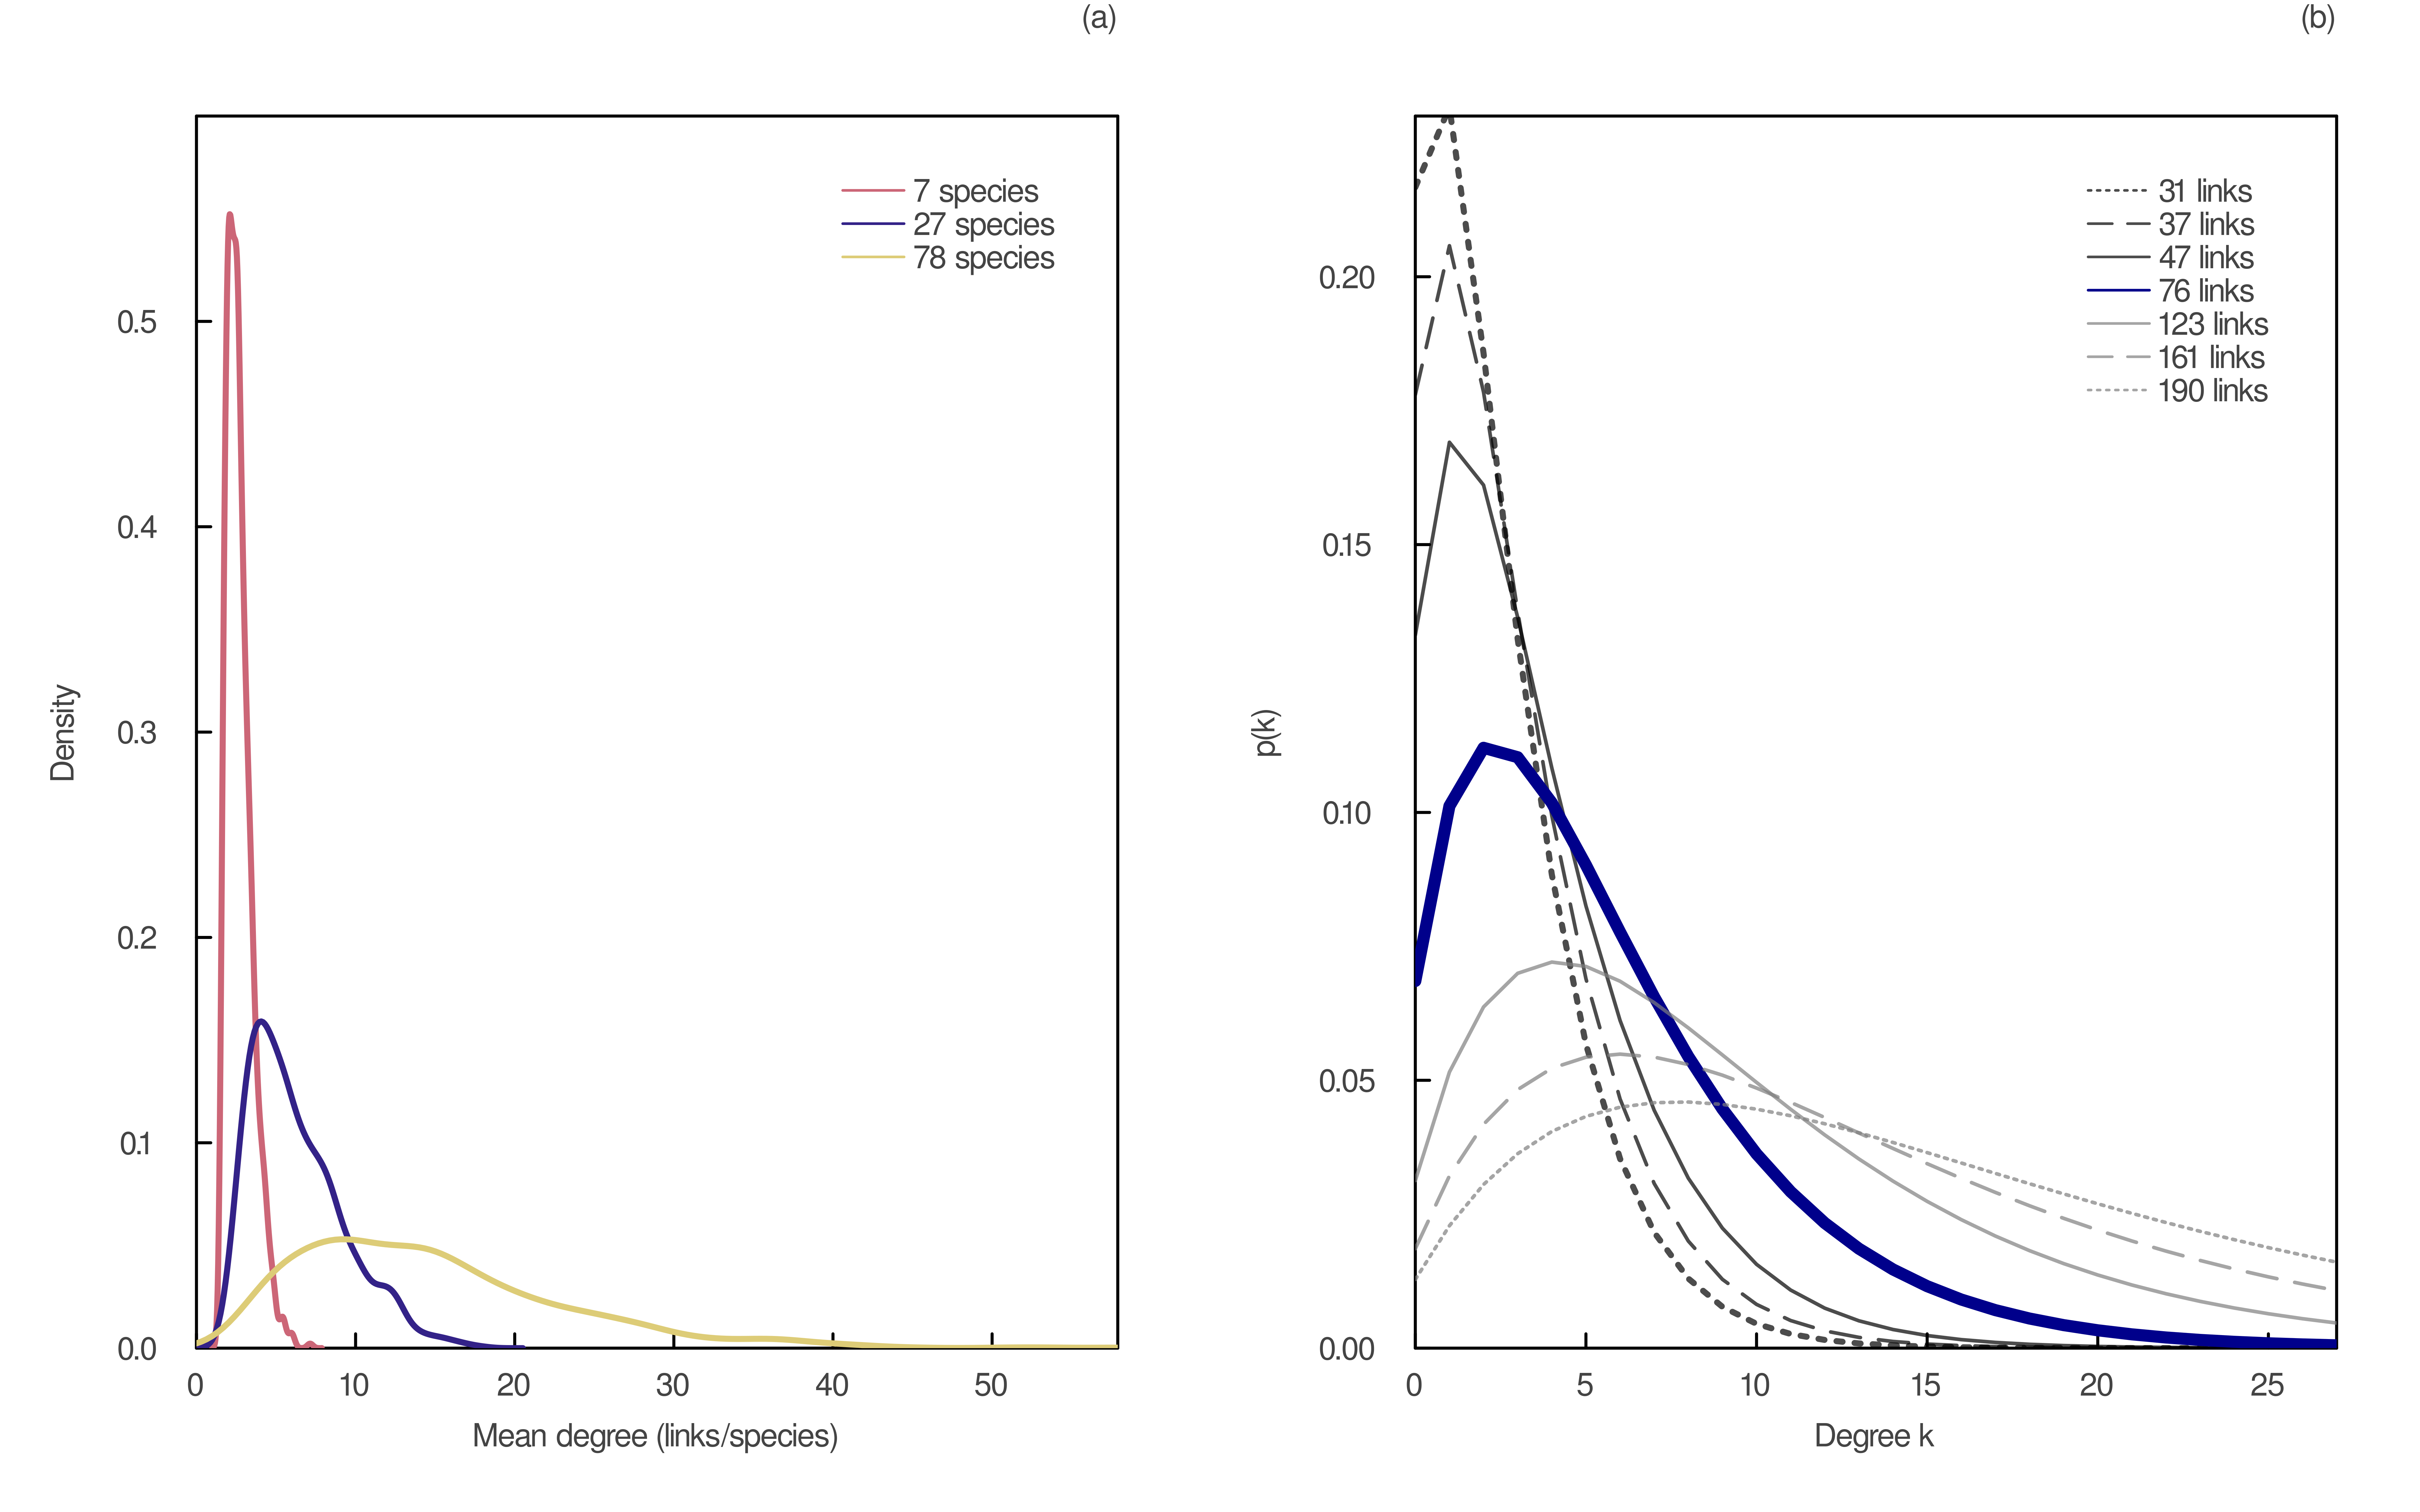
\includegraphics[width=\textwidth]{figures/article2/maxent_degree_dist_fl.png}
\captionsetup{justification=justified}
\captionof{figure}{\textbf{Maximum entropy degree distributions with predicted numbers of interactions.}
(a) Probability density of the mean degree of a food web obtained using
different values of species richness $S$. The number of interactions $L$ was
simulated $1000$ times using the flexible links model fitted to all empirical
networks. The mean degrees $2L/S$ were then obtained
from these simulated values. (b) Degree distributions of maximum entropy for a
network of $S=27$ species and different numbers of interactions. The numbers
of interactions correspond to the lower and upper bounds of the $67\%$,
$89\%$, and $97\%$ percentile intervals (PI), as well as the median (in blue),
of the counterfactuals of the flexible links model. Each degree distribution
of maximum entropy was obtained using Eq~\ref{eq:lagrange_dd} after solving
numerically Eq~\ref{eq:lagrange2_dd} using different values of the mean
degree constraint.}
\label{fig:degree_dist_fl}

\end{box3.1}

\addcontentsline{toc}{section}{Box 3.2: Corresponding null and neutral models}

\newtcolorbox{box3.2}{colback=green!4,enhanced,title=Box \customlabel{box3.2}{3.2}: Corresponding null and neutral models,
	attach boxed title to top left={xshift=-4mm},boxrule=0pt,after skip=1cm,before skip=1cm,right skip=0cm,breakable,fonttitle=\bfseries,toprule=0pt,bottomrule=2pt,rightrule=0.5pt,leftrule=2pt,arc=0mm,skin=enhancedlast jigsaw,sharp corners,colframe=gree,colbacktitle=gre,boxed title style={
		frame code={ 
			\fill[gre](frame.south west)--(frame.north west)--(frame.north east)--([xshift=3mm]frame.east)--(frame.south east)--cycle;
			\draw[line width=1mm,gre]([xshift=2mm]frame.north east)--([xshift=5mm]frame.east)--([xshift=2mm]frame.south east);
			
			\draw[line width=1mm,gre]([xshift=5mm]frame.north east)--([xshift=8mm]frame.east)--([xshift=5mm]frame.south east);
			\fill[green!40](frame.south west)--+(4mm,-2mm)--+(4mm,2mm)--cycle;
		}
	}
}

\begin{box3.2}

\textbf{Null models (types I and II)}

The predictions of our heuristic maximum entropy models were compared against
two topological null models. These null models use the same ecological
information as our heuristic models and thus constitute an adequate baseline for
comparison. The first is the type I null model of \textcite{Fortuna2006Habitat}, in
which the probability that a species $i$ predates on another species $j$ is
given by
  
\begin{eqnarray}
\label{eq:type1null}
    p(i \rightarrow j) = \frac{L}{S^2}.
\end{eqnarray}
  
The second is the type II null model of \textcite{Bascompte2003Nested}, in which
the probability of interaction is instead given by 
  
\begin{eqnarray}
\label{eq:type2null}
    p(i \rightarrow j) = \frac{1}{2} \left(\frac{k_{in}(j)}{S} +
    \frac{k_{out}(i)}{S}\right),
\end{eqnarray}
  
where $k_{in}(j)$ and $k_{out}(i)$ are the in and out-degrees of species $j$ and
$i$, respectively. The type I null model is based on connectance, whereas the
type II null model is based on the joint degree sequence. Therefore, the type I
and II topological null models correspond to our type I and II heuristic MaxEnt
models, respectively, since they use similar constraints. 
  
We generated probabilistic networks using both types of null models for all
empirical food webs in our complete dataset. Then, we converted these networks
to adjacency matrices of Boolean values by generating $100$ random networks for
each of these probabilistic webs and kept the $L$ entries that were sampled the
most amount of times, with $L$ given by the number of interactions in each food
web. This ensured that the resulting null networks had the same number of
interactions as their empirical counterparts. Thus, for each null model, we
ended up with one null adjacency matrix for each empirical network. \\

\textbf{Neutral model}
  
We also compared our heuristic MaxEnt models to a neutral model of relative
abundances, in which the probabilities of interaction are given by
  
\begin{eqnarray}
\label{eq:neutralmodel}
    p(i \rightarrow j) \propto \frac{n_i}{N} \times \frac{n_j}{N},
\end{eqnarray}
  
where $n_i$ and $n_j$ are the abundances (or biomass) of both species and $N$ is
the total abundance (or biomass) of all species in the network. We generated
neutral abundance matrices for all empirical food webs in our abundance dataset
and converted these weighted networks to adjacency matrices of Boolean values
using the same method as the one we used for our null models. 

\end{box3.2}

\section{Results and Discussion}

\subsection{Analytical maximum entropy models}

We first discuss the predictive capacity of our analytical models. The
relationship between the relative numbers of prey $k_{out}$ and predators
$k_{in}$ in empirical networks and obtained from the joint degree distributions
of maximum entropy is depicted in the left and central panels of
Figure~\ref{fig:joint_dd}, respectively. We observe that our analytical model predicts
higher values of generality and vulnerability compared to empirical food webs
(i.e. relative values of $k_{out}$ and $k_{in}$ both closer to $1$) for many
species. In other words, our model predicts that species that have many
predators also have more prey than what is observed empirically (and
conversely). This is not surprising, given that our model did not include
biological factors preventing generalist predators from having many prey.
Nevertheless, with the exception of these generalist species, MaxEnt adequately
predicts that most species have low generality and vulnerability values.

\afterpage{\clearpage

\begin{figure}[!h]
  \centering
  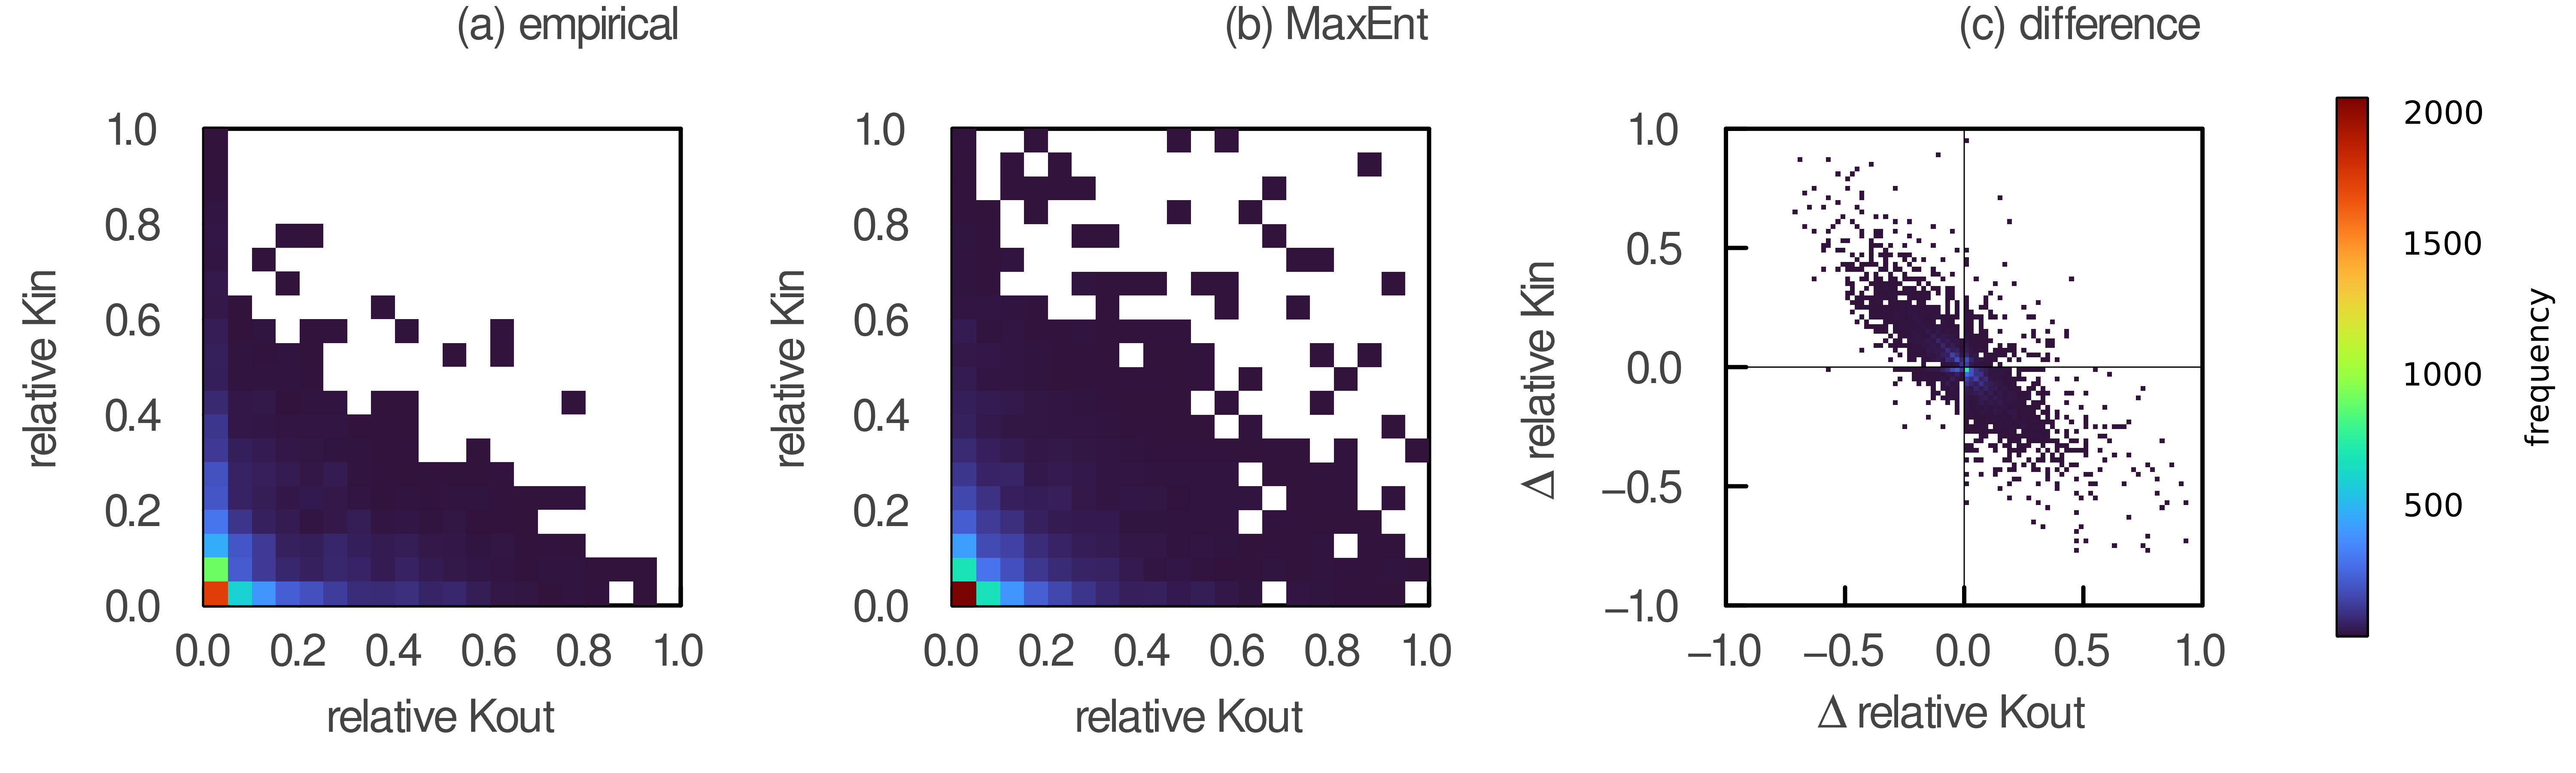
\includegraphics[width=\textwidth]{figures/article2/joint_degree_dist.png}
  \caption{\textbf{Prediction errors of the relative number of predators and prey.}
  The relative number of predators ($k_{in}$) is plotted against the relative
  number of prey ($k_{out}$) for each species in all (a) empirical and (b)
  predicted joint degree sequences. The predicted joint degree sequences were
  obtained after sampling one realization of the joint degree distribution of
  maximum entropy for each network while keeping the total number of
  interactions constant. (c) Difference between predicted and empirical values
  when species are ordered according to their total degree. Due to significant
  data overlap, all relationships are represented as 2D histograms. The color
  bar indicates the number of species that fall within each bin.}
\label{fig:joint_dd}
\end{figure}

}

Examining the difference between predicted and empirical values for each species
gives a slightly different perspective (right panel of Figure~\ref{fig:joint_dd}).
To make that comparison, we must first associate each of our predictions with a
specific species in a network. Indeed, our predicted joint degree sequences have
the same number of species (elements) as their empirical counterparts, but they
are species agnostic. In other words, instead of predicting a pair of values for
each species directly (i.e. the number of prey and predators of a given species
$i$), we predicted the entire joint degree sequence without taking into account
species' identity (i.e. the distribution of the number of prey and predators for
the entire set of species, without knowing which values belong to which
species). The challenge is thus to adequately associate predictions with
empirical data. In Figure~\ref{fig:joint_dd}, we present these differences when
species are ordered by their total degree in their respective networks (i.e. by
the sum of their in and out-degrees). This means that the species with the
highest total degree in its network will be associated with the highest
prediction, and so forth. Doing so, we see that species predicted to have a
higher number of predators than what is observed generally have a lower number
of prey than what is observed (and conversely). This is also shown in
Figure~\ref{fig:kin_kout_diff_strata} (Appendix~\ref{supp:B}), which represents the
relationship between prediction errors in the \textit{absolute} (non-relative)
values of $k_{out}$ and $k_{in}$ across networks of varying levels of species
richness. This is because the difference in total degree ($k_{out} + k_{in}$)
between predictions and empirical data is minimized when species are ranked by
their total degree (i.e. the average deviation of the sum of relative $k_{out}$
and $k_{in}$ is close to $0$ across all species). This result thus shows that
the difference between predicted and empirical total degrees is low for most
species when ordered by their total degrees. There are no apparent biases
towards in or out degrees. In Figure~\ref{fig:kin_kout_diff}
(Appendix~\ref{supp:B}), we show how these differences change when species are
instead ordered by their out-degrees (left panel) and in-degrees (right panel),
i.e. when minimizing the error in the estimation of the out and in-degrees,
respectively.

Another way to evaluate the empirical support of the sampled joint degree
sequences is to compare their shape with the ones of empirical food webs. We
described the shape of a joint degree sequence by measuring the distance between
its in and out-degree sequences (i.e. the distance between its marginal
distributions). To do so, we calculated the Kullback–Leibler (KL) divergence
(\cite{Kullback1951Information}) between the in and out-degree sequences of each
predicted and empirical distribution. The KL divergence is a measure of relative
entropy describing the difference between two distributions. Low values indicate
high similarity between the in and out-degree sequences and suggest that the
joint degree sequence has a high level of symmetry. We compared the shape of the
empirical and predicted joint degree sequences in the left panel of
Figure~\ref{fig:kl_diverg}. As expected, our model predicts more similar in-degree and
out-degree sequences than empirical data (shown by lower KL divergence values).
However, the difference between the KL divergence of predicted and empirical
joint degree sequences decreases with connectance (right panel of
Figure~\ref{fig:kl_diverg}). This might be because food webs with a low connectance are
harder to predict than food webs with a high connectance. Indeed, in low
connectance systems, what makes two species interact may be more important for
prediction than in high connectance systems, in which what prevents species from
interacting may be more meaningful. This implies that more ecological
information may be needed in food webs with a low connectance because more
ecological processes determine interactions compared to non-interactions.
Therefore, other ecological constraints might be needed to account for the
asymmetry of the joint degree distribution, especially for networks with a lower
connectance. Nevertheless, our MaxEnt model seems to capture quite well the
shape of the joint degree sequence for networks having a high connectance.

\afterpage{\clearpage

\begin{figure}[!h]
  \centering
  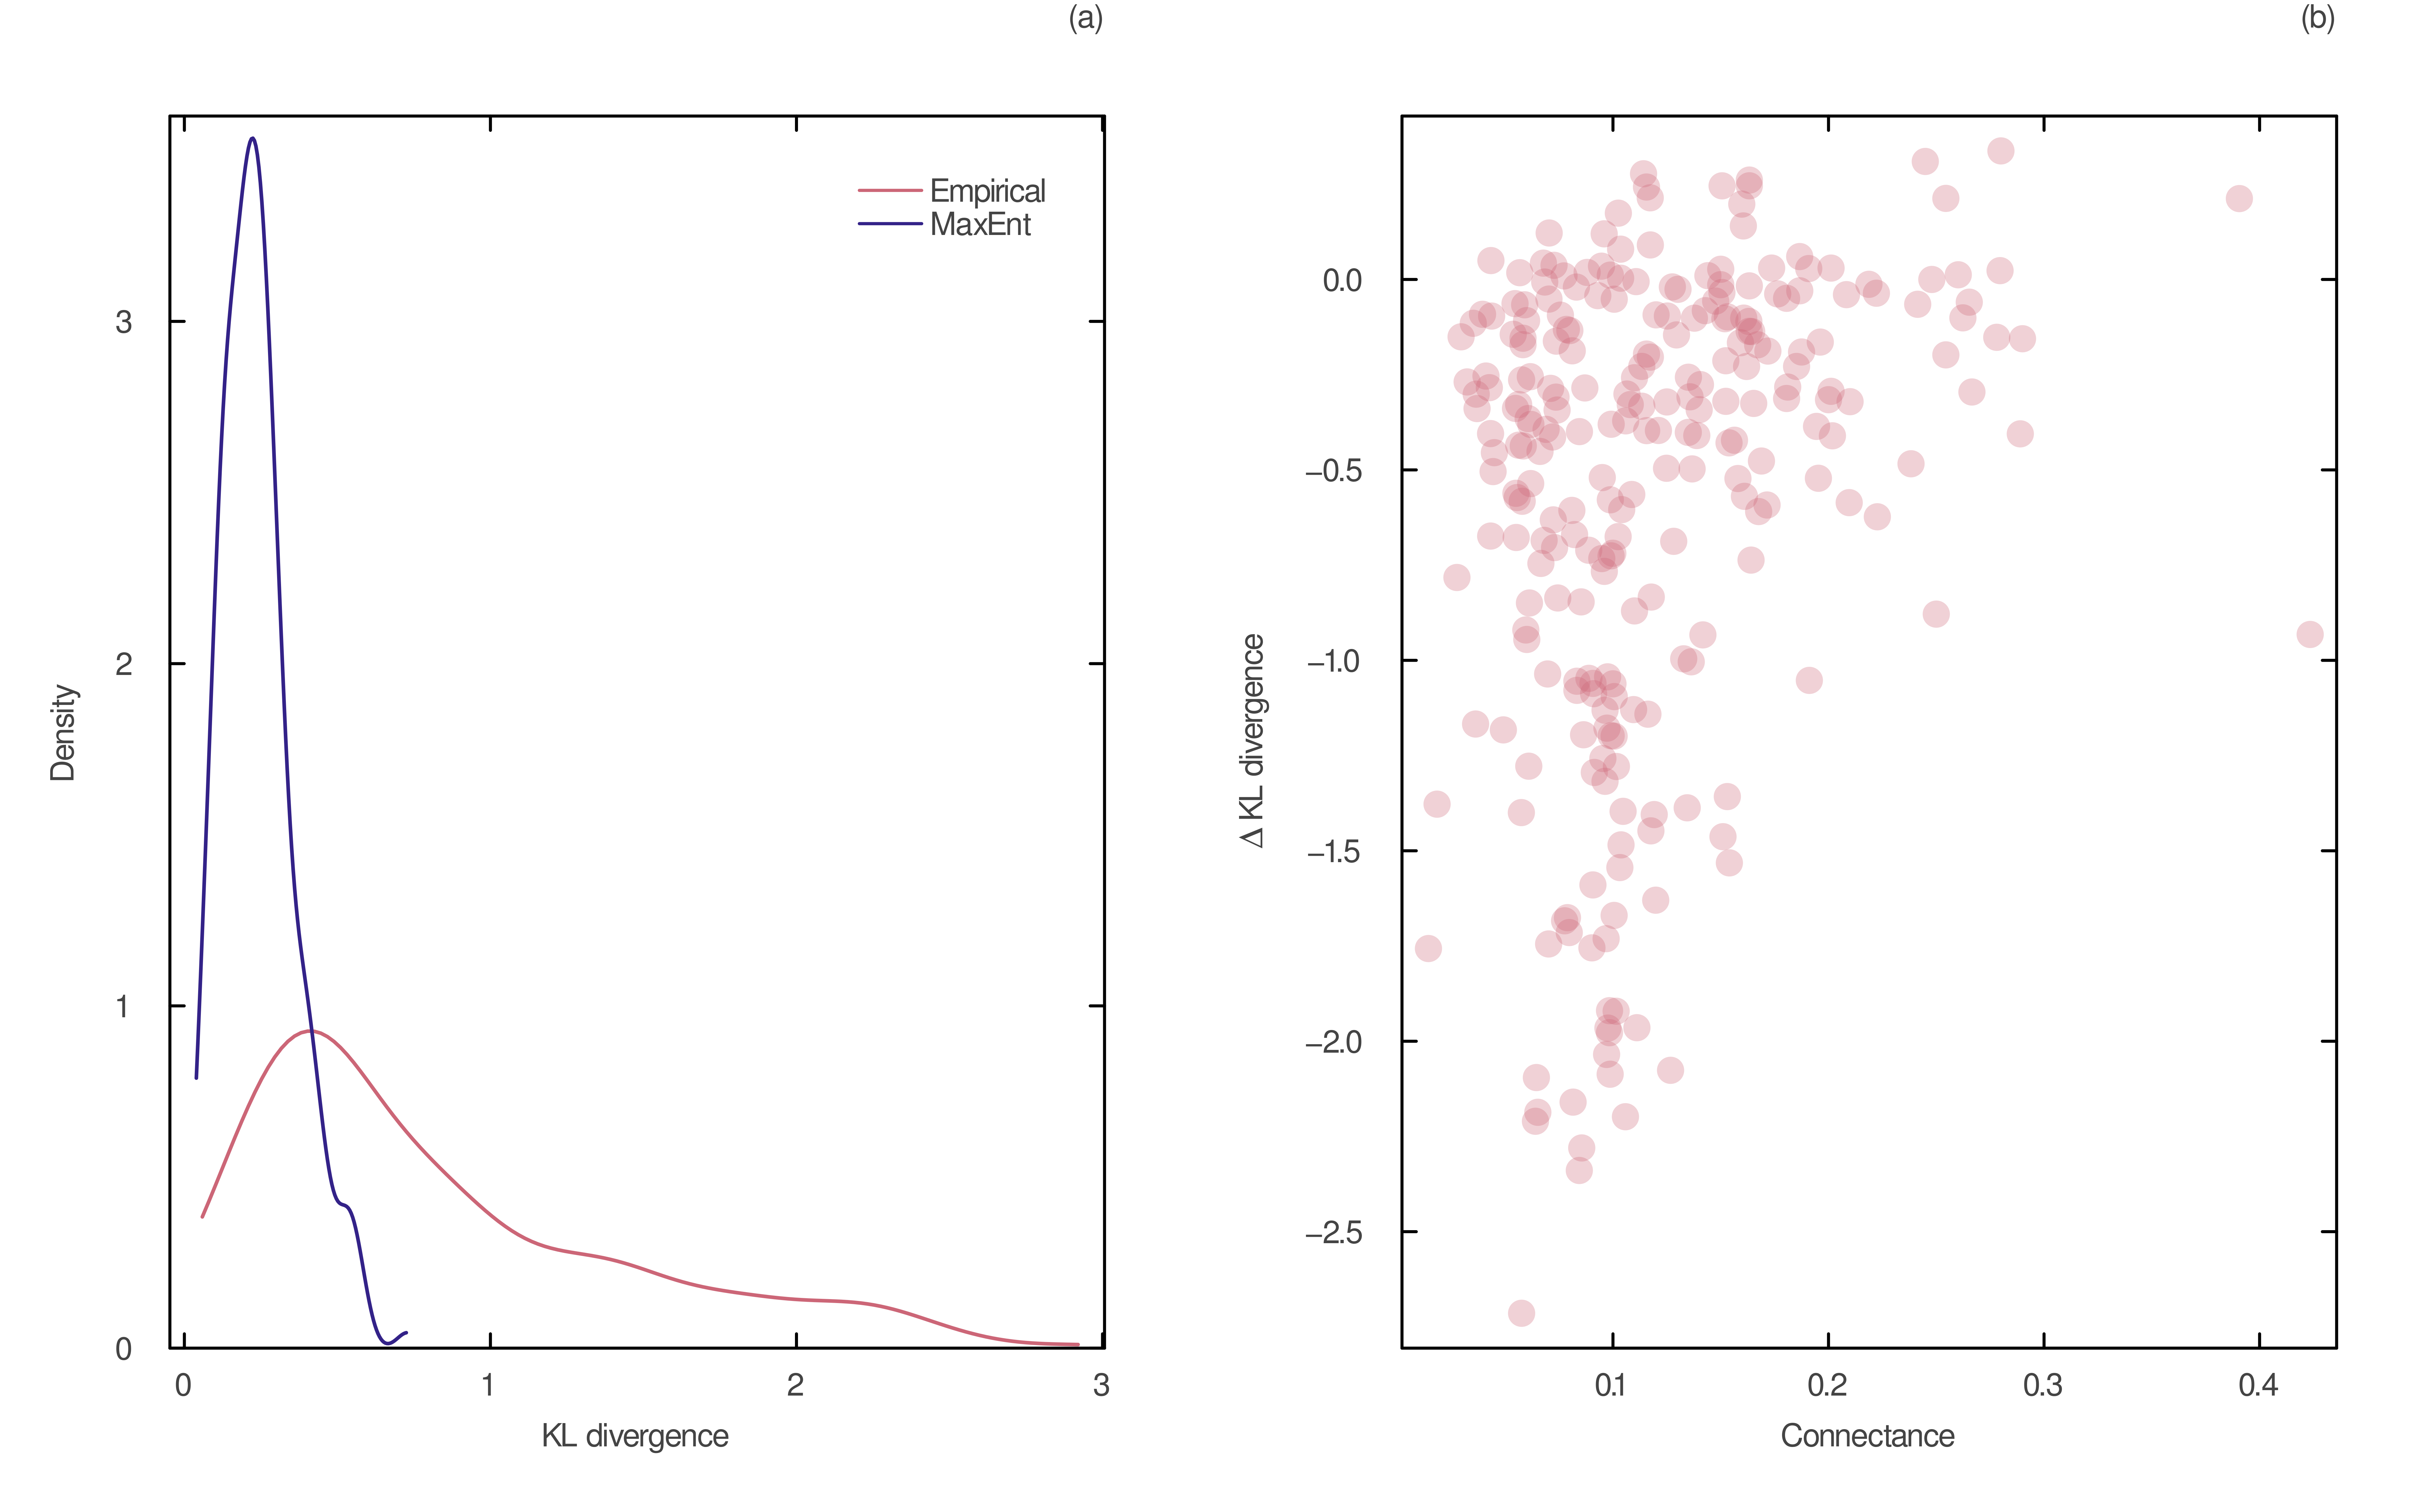
\includegraphics[width=\textwidth]{figures/article2/kl_divergence.png}
  \caption{\textbf{Shape of empirical and predicted joint degree sequences.}
  (a) Probability density of KL divergence between in and out-degree sequences of
  empirical and predicted joint degree sequences. (b) Difference between the KL
  divergence of empirical and predicted joint degree sequences as a function of
  connectance. The predicted joint degree sequences were obtained after sampling
  one realization of the joint degree distribution of maximum entropy for each
  network while keeping the total number of interactions constant.}
\label{fig:kl_diverg}
\end{figure}

}

Regarding the degree distribution of maximum entropy, one aspect that informs us
of its ecological realism is the number of isolated species it predicts. As
\textcite{MacDonald2020Revisiting} pointed out, the size of food webs should at
least be of $S-1$ interactions since a lower number would yield isolated
species, i.e. species without any predator or prey. Because non-basal species
must eat to survive, isolated species could indicate that other species are
missing; otherwise, isolated species should be removed from the network. In
Figure~\ref{fig:heatmap} (Appendix~\ref{supp:B}), we show that the degree
distribution of maximum entropy, given $S$ and $L$, gives a very low probability
that a species will be isolated in its food web (i.e. having $k = 0$) when $L >
S-1$. However, under our purely information-theoretic model, the probability
that a species is isolated is quite high when the total number of interactions
is below $S-1$. Moreover, the expected proportion of isolated species rapidly
declines by orders of magnitude with increasing numbers of species and
interactions. This supports the ecological realism of the degree distribution of
maximum entropy derived above. Nevertheless, ecologists wanting to model a
system without allowing isolated species could simply change the lower limit of
$k$ to $1$ in Eq~\ref{eq:lagrange2_dd} and solve the resulting equation
numerically.

\subsection{Heuristic maximum entropy models}

In this section, we explore the predictions of our heuristic models. Overall, we
found that the models based on the joint degree sequence (i.e. the type II null
and heuristic MaxEnt models) reproduced the structure of empirical food webs
much better than the ones based on connectance (i.e. the type I null and
heuristic MaxEnt models, Table~\ref{tbl:measures_all}). This suggests that the
predictive capacity of connectance might be more limited than what was
previously suggested (\cite{Poisot2014When}). On the other hand, the neutral
model of relative abundances was surprisingly good at predicting the maximum
trophic level and the network diameter (Table~\ref{tbl:measures_abund}). However,
with the exception of the network diameter, the type II heuristic MaxEnt model
was better at predicting network structure than the neutral model for most
measures considered. This might be because, although neutral processes are
important, they act in concert with niche processes in determining species
interactions (\cite{Bartomeus2016Common}, \cite{Canard2014Empirical},
\cite{Poisot2015Species}, \cite{Pomeranz2019Inferring}). The joint degree sequence
captures information on both neutral and niche processes because the number of
prey and predators a species has is determined by its relative abundance and
biological traits. These results thus show that having information on the number
of prey and predators for each species substantially improves the prediction of
food-web structure, both compared to models solely based on connectance and to
the ones solely based on species relative abundances.

\afterpage{\clearpage

\begin{table}[!h]
  \resizebox{\textwidth}{!}{
  \centering
  \begin{tabular}{c c c c c c c c } 
   \hline
   {\bf model} & {\bf $\rho$} & {\bf maxtl} & {\bf diam} & {\bf MxSim} & {\bf
  Cannib} & {\bf Omniv} & {\bf entropy} \\
  \hline
  null 1 & -0.167 &  0.980 & 1.428 & -0.502 &  2.007 & 1.493 & 0.056 \\ 
  MaxEnt 1 & -0.226 & 0.831 & 1.274 & -0.524 & 1.982 & 1.863 & 0.106 \\ 
  null 2 & 0.160 & -0.125 & 0.016 & 0.007 & 1.078 & 0.559 & -0.023 \\ 
  MaxEnt 2 & -0.015 & 0.178 & 0.565 & -0.282 & 0.698 & 0.589 & 0.058 \\ 
  \hline
  \end{tabular}
  }
  \caption{\textbf{Standardized mean difference between predicted network measures
and empirical data for all food webs in our complete dataset ($N = 257$).} Positive (negative) values indicate that the measure is
overestimated (underestimated) on average. Null 1: Type I null model based on
connectance. MaxEnt 1: Type I heuristic MaxEnt model based on connectance.
Null 2: Type II null model based on the joint degree sequence. MaxEnt 2: Type
II heuristic MaxEnt model based on the joint degree sequence. $\rho$:
nestedness measured by the spectral radius of the adjacency matrix.
\textit{maxtl}: maximum trophic level. \textit{diam}: network diameter.
\textit{MxSim}: average maximum similarity between species pairs.
\textit{Cannib}: proportion of cannibal species (self-loops). \textit{Omniv}:
proportion of omnivorous species. \textit{entropy}: SVD entropy.}
  \label{tbl:measures_all}
\end{table}

\hfill \break
\hfill \break

\begin{table}[!h]
  \resizebox{\textwidth}{!}{
  \centering
  \begin{tabular}{c c c c c c c c } 
   \hline
   {\bf model} & {\bf $\rho$} & {\bf maxtl} & {\bf diam} & {\bf MxSim} & {\bf Cannib} & {\bf Omniv} & {\bf entropy} \\
  \hline
  neutral & 0.367 & -0.090 & 0.027 & 0.266 & 6.870 & 0.576 & -0.083 \\ 
  null 1 & -0.134 & 0.950 & 1.919 & -0.369 & 2.077 & 0.614 & 0.068 \\ 
  MaxEnt 1 & -0.229 & 1.020 & 1.946 & -0.355 & 2.215 & 0.801 & 0.121 \\ 
  null 2 & 0.128 & -0.115 & -0.135 & 0.157 & 1.444 & 0.029 & -0.021 \\ 
  MaxEnt 2 & -0.010 & 0.054 & 0.243 & -0.062 & -0.038 & 0.083 & 0.038 \\ 
  \hline
  \end{tabular}
  }
  \caption{\textbf{Standardized mean difference between predicted network measures and empirical data for all food webs in our abundance dataset ($N = 19$).} Positive (negative) values indicate that the measure is
overestimated (underestimated) on average. Null 1: Type I null model based on
connectance. MaxEnt 1: Type I heuristic MaxEnt model based on connectance.
Null 2: Type II null model based on the joint degree sequence. MaxEnt 2: Type
II heuristic MaxEnt model based on the joint degree sequence. $\rho$:
nestedness measured by the spectral radius of the adjacency matrix.
\textit{maxtl}: maximum trophic level. \textit{diam}: network diameter.
\textit{MxSim}: average maximum similarity between species pairs.
\textit{Cannib}: proportion of cannibal species (self-loops). \textit{Omniv}:
proportion of omnivorous species. \textit{entropy}: SVD entropy.}
  \label{tbl:measures_abund}
\end{table}

\clearpage
}

Next, the predictions of the type II heuristic MaxEnt model can be compared to
its null model counterpart. On average, the type II heuristic MaxEnt model was
better at predicting nestedness ($0.62 \pm 0.08$) than its corresponding null
model ($0.73 \pm 0.05$; empirical networks: $0.63 \pm 0.09$) for networks in our
complete dataset (Table~\ref{tbl:measures_all}). This might in part be due to the
fact that nestedness was calculated using the spectral radius of the adjacency
matrix, which directly leverages information on the network itself just like the
heuristic MaxEnt model. The proportion of self-loops (cannibal species) was also
better predicted by the type II heuristic MaxEnt model in comparison to the type
II null model. However, the type II null model was better at predicting network
diameter and average maximum similarity between species pairs, and predictions
of the maximum trophic level and the proportion of omnivorous species were
similar between both types of models. We believe that this is because increasing
the complexity of a food web might increase its average and maximum food-chain
lengths. In comparison, the null model was more stochastic and does not
necessarily produce more complex food webs with longer food-chain lengths. 

Moreover, we found that the entropy of empirical food webs was slightly lower
than their maximum entropy when constrained by their joint degree sequence
(Figure~\ref{fig:entropy_dist}, Appendix~\ref{supp:B}). Empirical food webs had an
SVD entropy of $0.89 \pm 0.04$, compared to an SVD entropy of $0.94 \pm 0.03$
for networks generated using the type II heuristic MaxEnt model. The
relationship between the SVD entropy of empirical food webs and their maximum
entropy is plotted in the last panel of Figure~\ref{fig:measures}. The slight
increase in entropy confirms that our method generated more complex networks.
Even though we found that many measures of empirical networks are close to the
ones of their maximum entropy configuration, the relatively low predictability
of entropy itself may be indicative of additional constraints shaping food-web
structure, especially for networks with low SVD entropy. Incorporating more
constraints into the model could increase its capacity to generate networks with
an adequate level of complexity, as shown by the decrease in predictive errors
of entropy of the type II heuristic MaxEnt model compared to the one based on
connectance (Table~\ref{tbl:measures_all}). Additionally, we found no clear
relationship between the increase in SVD entropy and the number of species, the
number of interactions, and connectance (Figure~\ref{fig:entropy_size},
Appendix~\ref{supp:B}). This suggests that our model captured the complexity of
small and large networks on a similar level and that its capacity to reproduce
food-web structure was unrelated to the order and size of the network. In other
words, the gap in entropy between empirical food webs and their maximum entropy
configuration may be the result of additional constraints that were not taken
into account in the model, regardless of the number of species and the number of
interactions. 

\afterpage{\clearpage

\begin{figure}[!h]
  \centering
  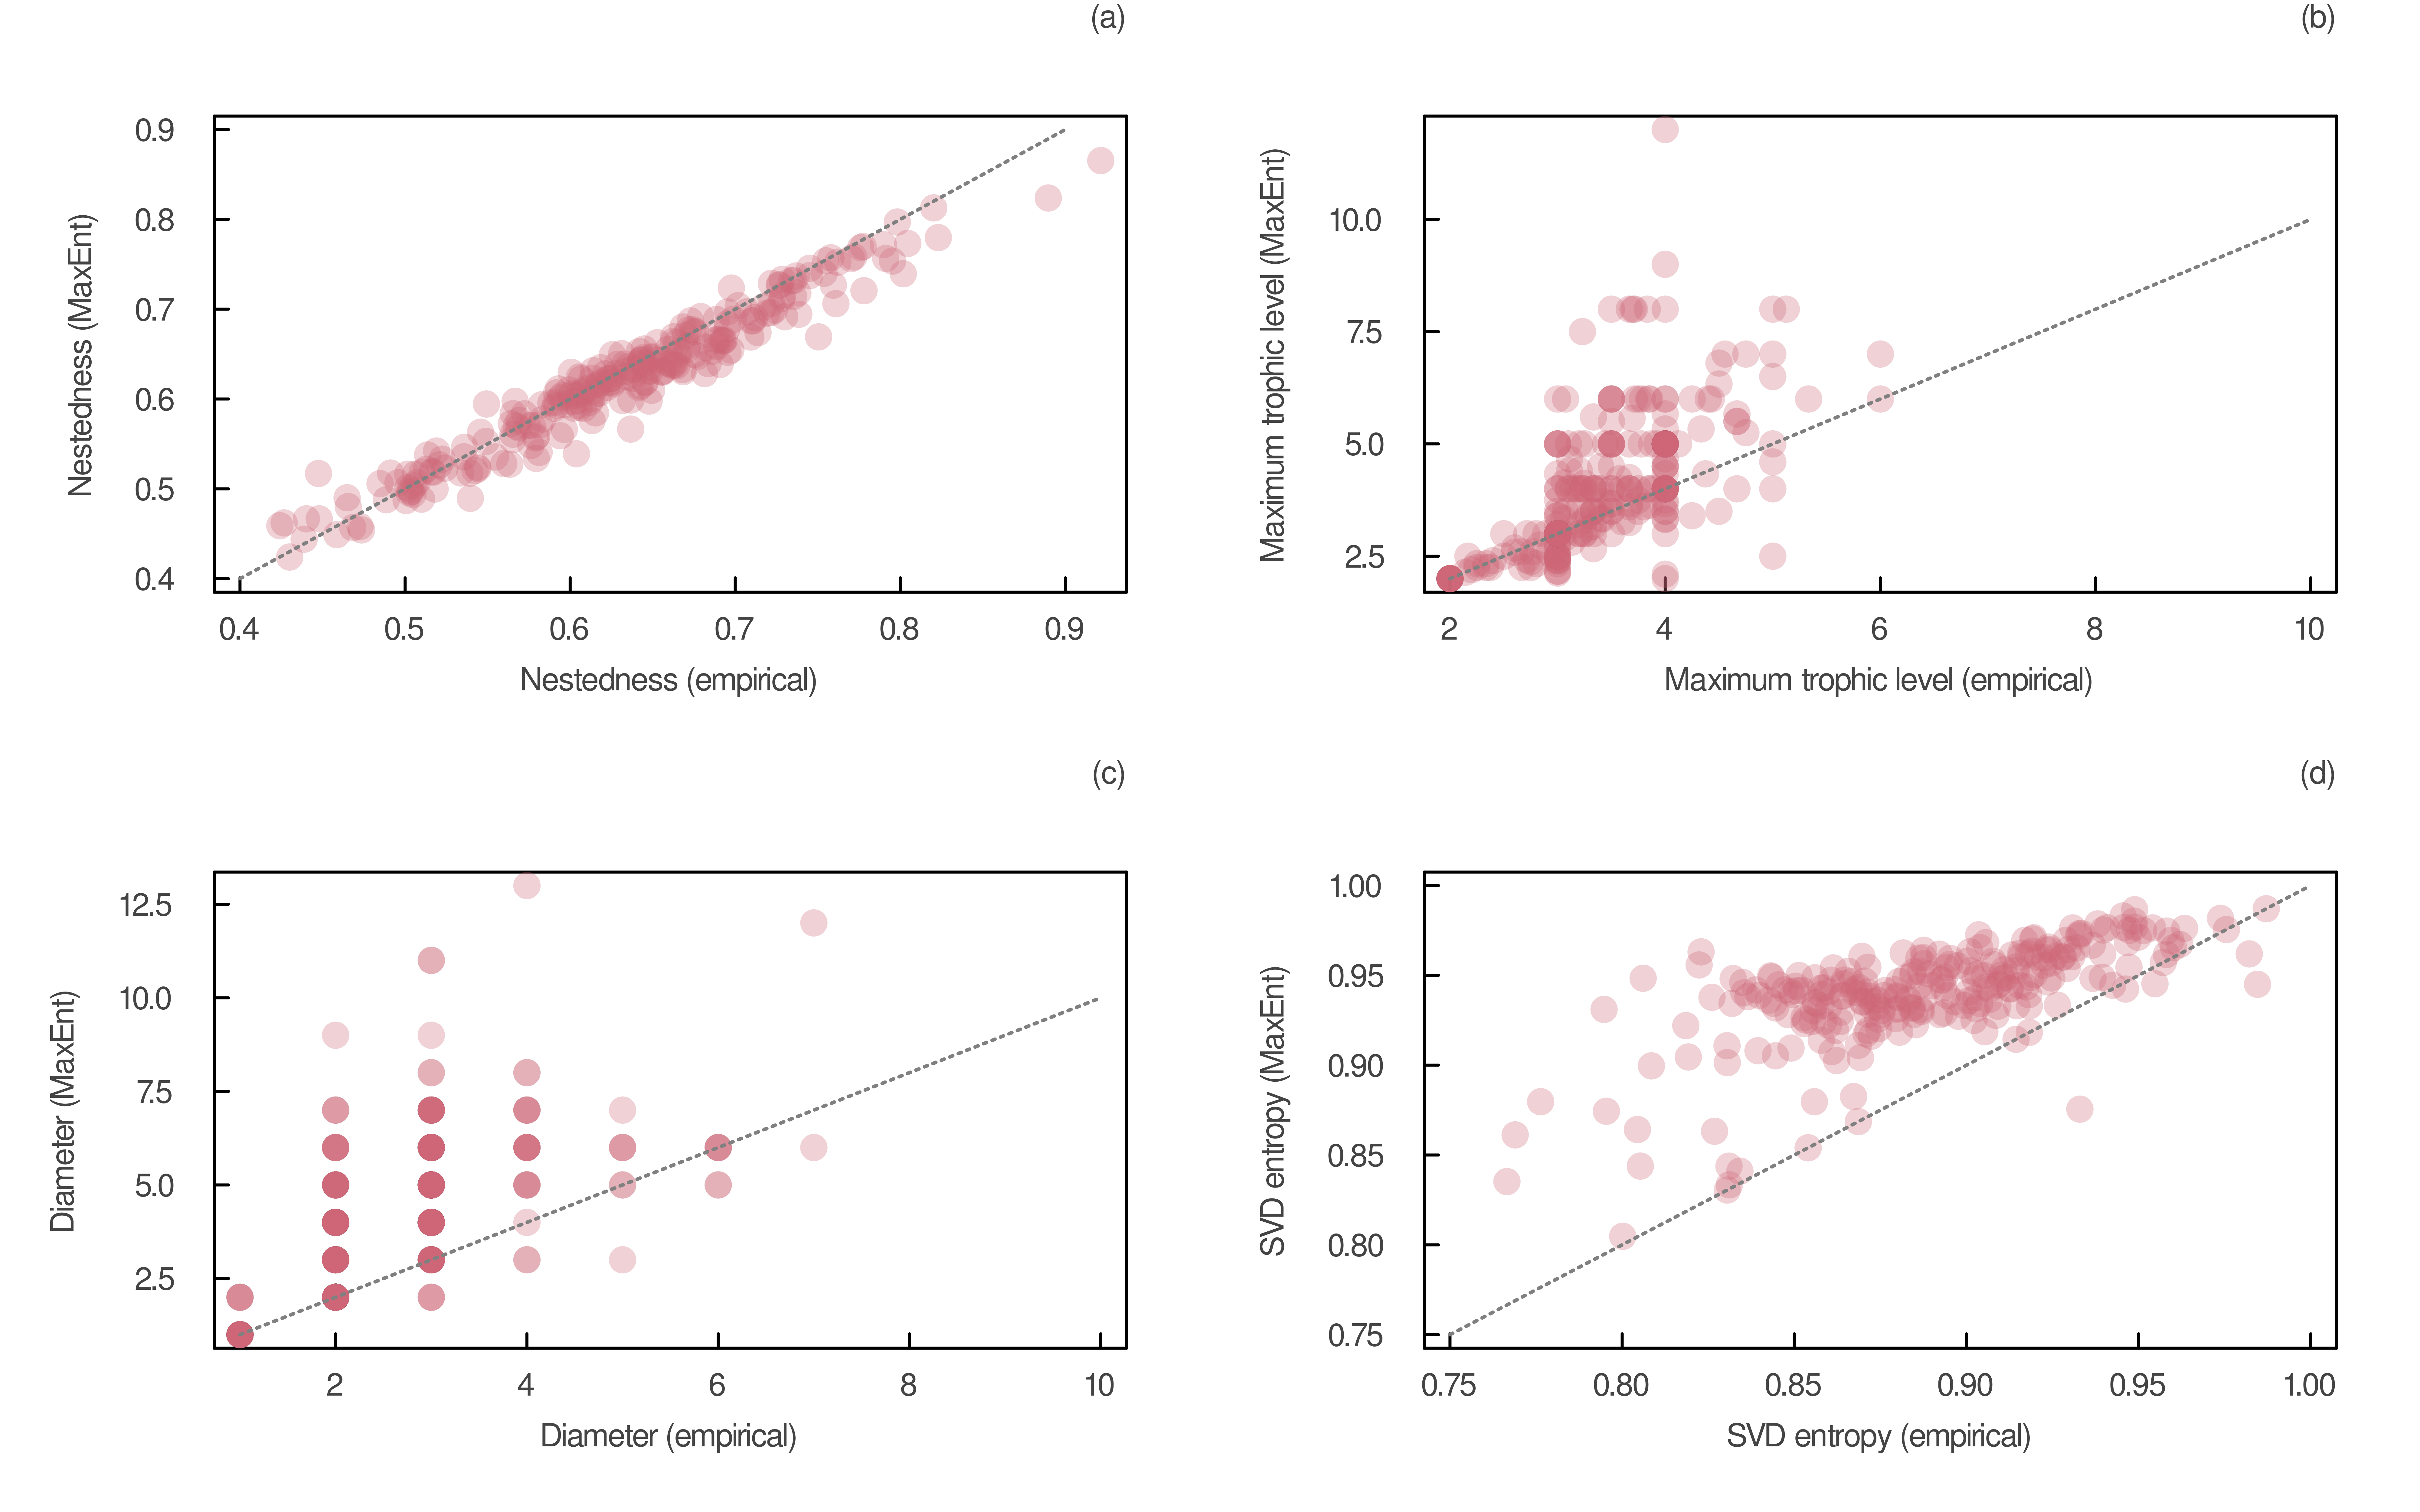
\includegraphics[width=\textwidth]{figures/article2/measures_emp_maxent.png}
  \caption{\textbf{Relationship between the structure of empirical and maximum entropy food webs.}
  Maximum entropy networks were obtained using the type II heuristic MaxEnt
  model based on the joint degree sequence. (a) Nestedness (estimated using the
  spectral radius of the adjacency matrix), (b) the maximum trophic level, (c)
  the network diameter, and (d) the SVD entropy were measured on these empirical
  and maximum entropy food webs. The identity line is plotted in each panel.}
  \label{fig:measures}
\end{figure}

}

A direct comparison of the structure of maximum entropy food webs constrained by
the joint degree sequence with empirical data also supports the results depicted
in Table~\ref{tbl:measures_all}. In Figure~\ref{fig:measures}, we show how well
empirical measures are predicted by the type II heuristic MaxEnt model.
Following our previous results, we found that nestedness was very well predicted
by our model. However, the model overestimated the maximum trophic level and
network diameter, especially when the sampled food web had intermediate values
of these measures. In Figure~\ref{fig:measures_richness} (Appendix~\ref{supp:B}),
we show that the pairwise relationships between the four measures in
Figure~\ref{fig:measures} and species richness in empirical food webs are similar
(in magnitude and sign) to the ones found in food webs generated using the type
II heuristic MaxEnt model. This indicates that the number of species in the
network does not seem to impact the ability of the model to reproduce food-web
structure. 

Notwithstanding its difficulties in reproducing adequate measures of food-chain
lengths, the type II heuristic MaxEnt model can predict surprisingly well the
proportions of three-species motifs in empirical food webs. Motifs have been
shown to be the backbone of complex ecological networks on which network
structure is built and play a crucial role in community dynamics and assembly
(\cite{Stouffer2011Compartmentalization}). Differences in motif profiles between an observed
food web and null model-generated ones can unveil important ecological
mechanisms that contribute to network structure (\cite{Stouffer2007Evidence}). In
Figure~\ref{fig:motifs}, we show that the motif profile of networks generated using the
type II heuristic MaxEnt model accurately reproduced the one of empirical data.
This model made significantly better predictions than the ones based on
connectance and the type II null model based on the joint degree sequence. This
is also shown in Figure~\ref{fig:motifs_rel}, which reveals that the relationships
between the proportions of single-link motifs in empirical food webs are similar
to the ones in networks generated using the type II heuristic MaxEnt model. This
is in contrast with the type I null and MaxEnt models based on connectance,
which produced opposite relationships than what was observed empirically. Our
findings show that generating the most complex food web constrained by the joint
degree sequence using maximum entropy does not alter the proportions of
three-species motifs on the whole. This suggests that motif profiles may simply
be a statistical attribute of food webs driven by the joint degree sequence.
However, given the incapacity of our MaxEnt models to accurately predict
food-chain lengths, the way motifs interconnect with each other may hold greater
biological significance than the proportion of motifs itself. 

\afterpage{\clearpage

\begin{figure}[!h]
  \centering
  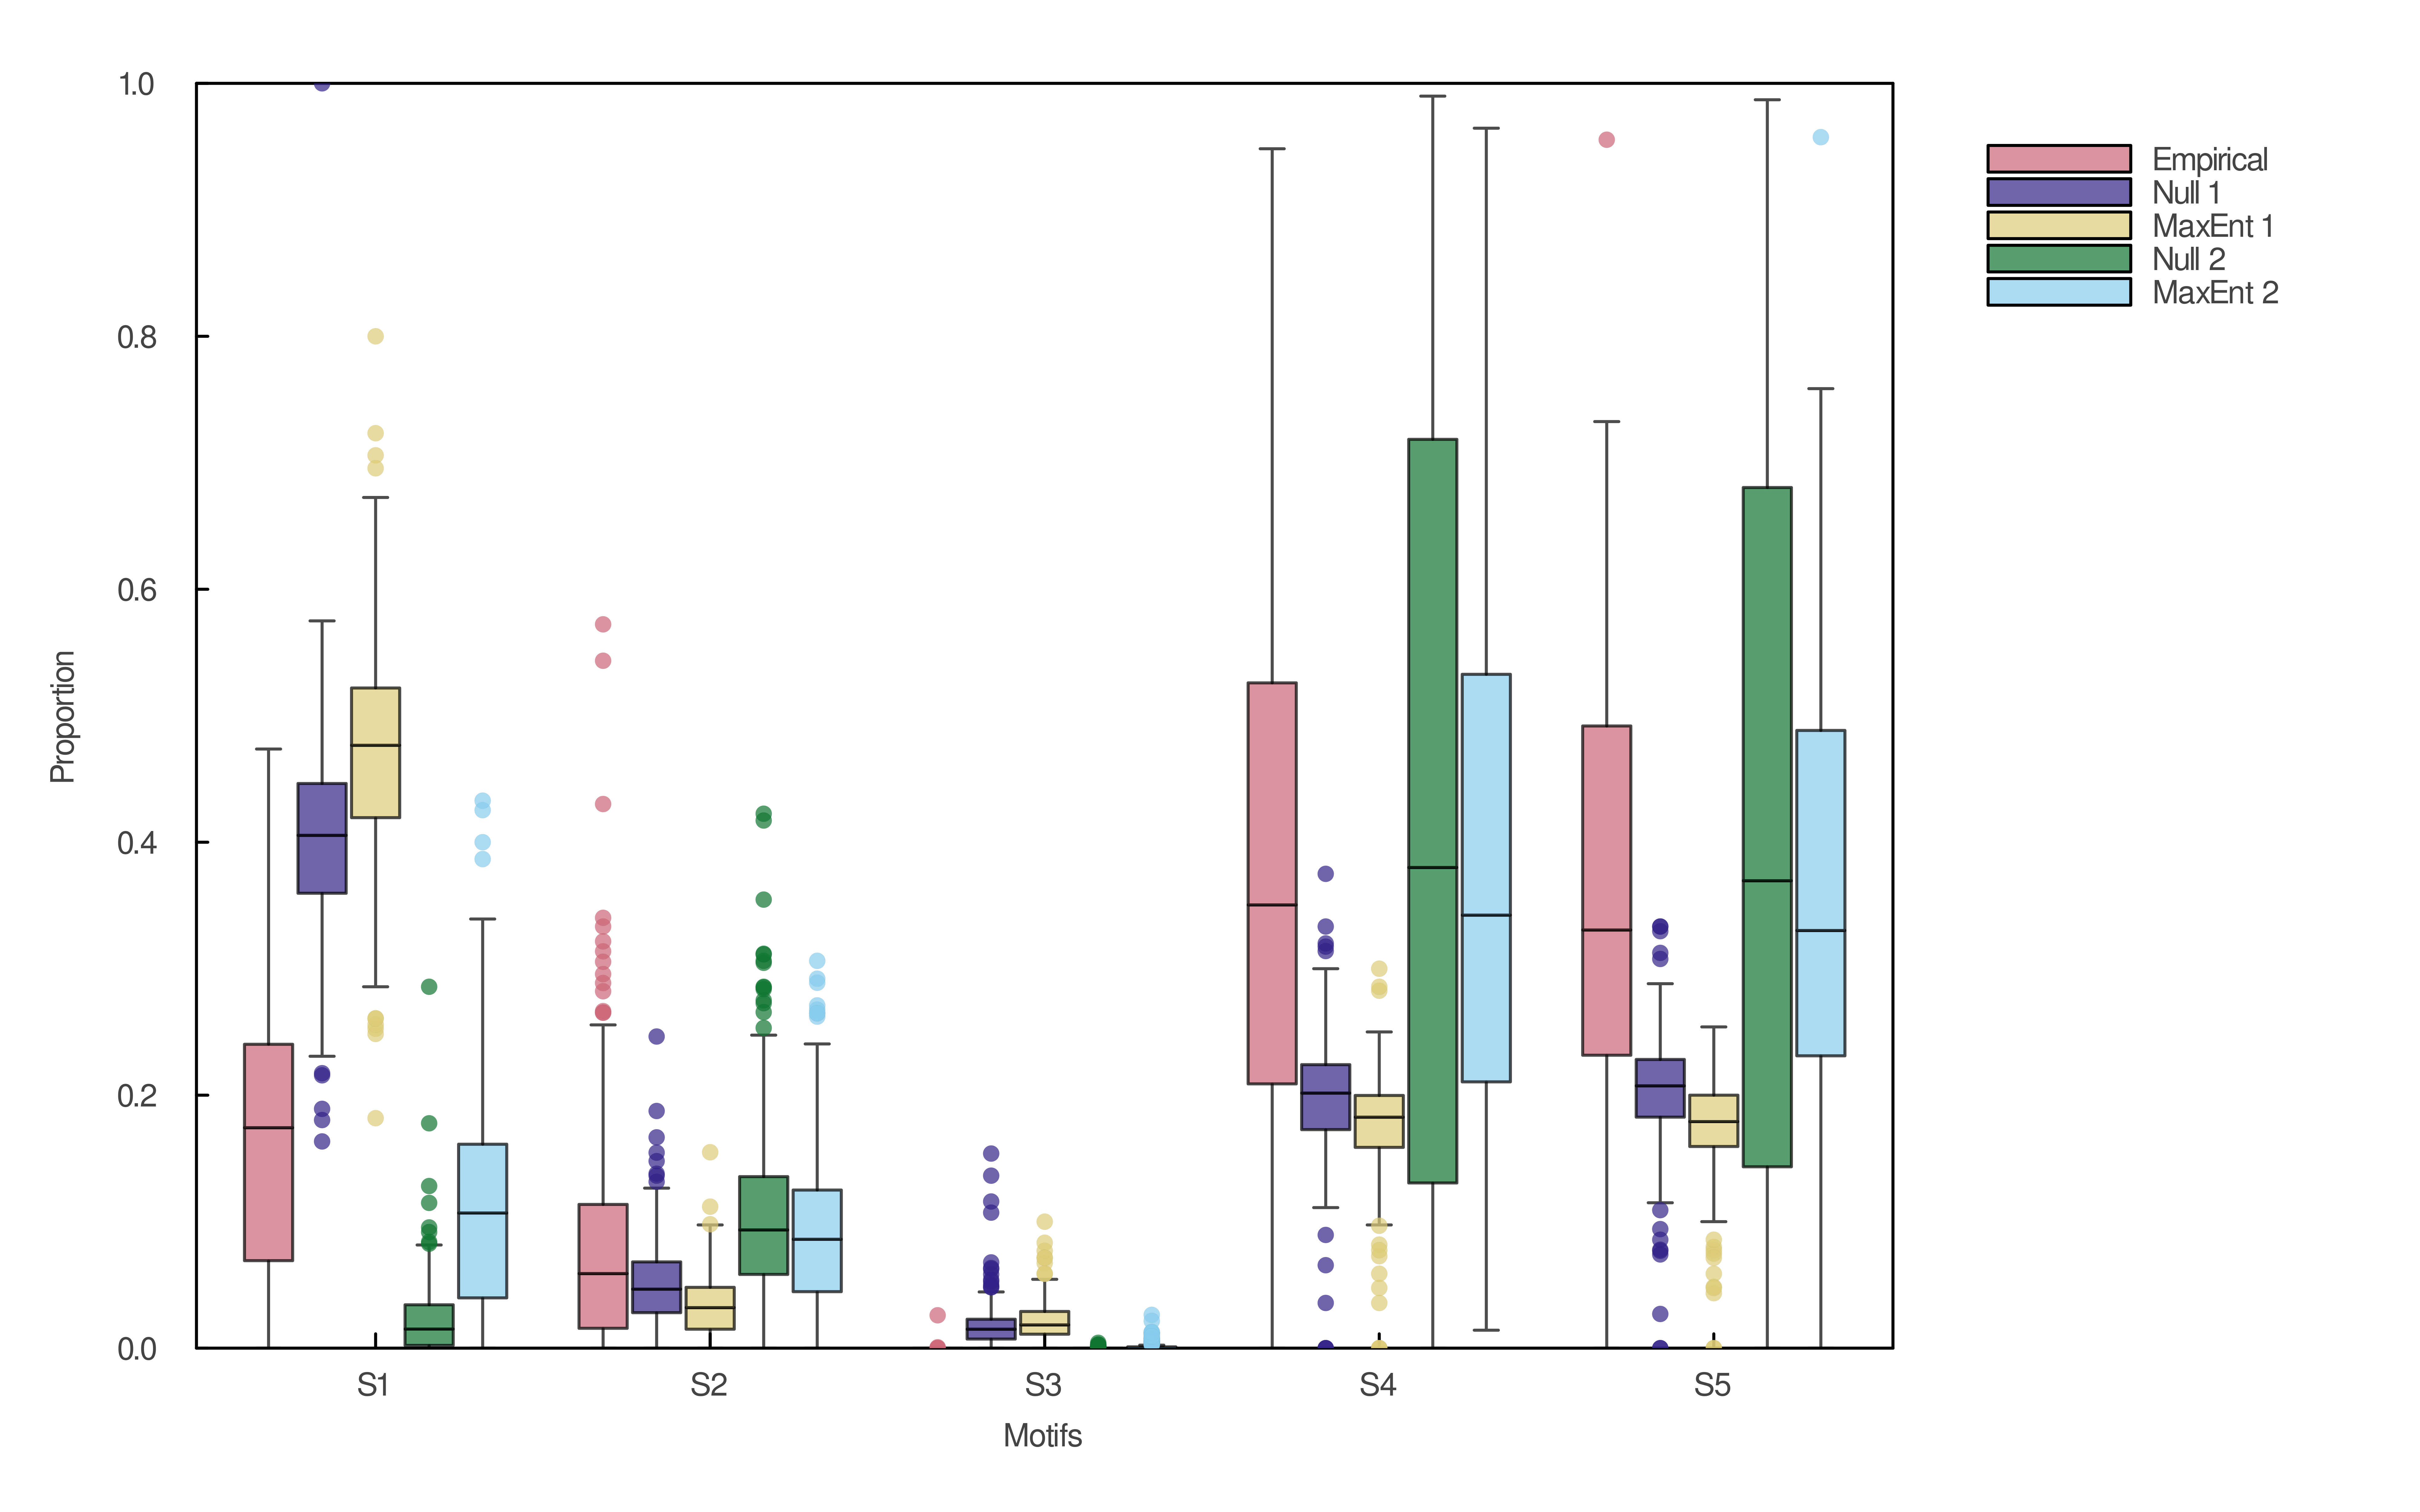
\includegraphics[width=\textwidth]{figures/article2/motifs_distribution.png}
  \caption{\textbf{Proportions of single-link three-species motifs in empirical and predicted food webs.}
  S1: Tri-trophic chain (a top predator feeds on a meso-predator which feeds on
  a basal prey). S2: Omnivory (a top predator feeds on a meso-predator and a
  basal prey). S3: Tri-trophic feeding loop (a cyclic three-species
  predator-prey system). S4: Apparent competition (a predator feeds on two
  prey). S5: Exploitative competition (two predators feed on the same prey).
  Null 1: Type I null model based on connectance. MaxEnt 1: Type I heuristic
  MaxEnt model based on connectance. Null 2: Type II null model based on the
  joint degree sequence. MaxEnt 2: Type II heuristic MaxEnt model based on the
  joint degree sequence. Boxplots display the median proportion of each motif in
  food webs (middle horizontal lines), as well as the first (bottom horizontal
  lines) and third (top horizontal lines) quartiles. Vertical lines encompass
  all data points that fall within $1.5$ times the interquartile range from both
  quartiles, and dots are data points that fall outside this range. Only the
  single-link motifs S1-S5 are shown given the scarcity of double-link motifs in
  most empirical and predicted networks. }
\label{fig:motifs}
\end{figure}

}

\afterpage{\clearpage

\begin{figure}[!h]
  \centering
  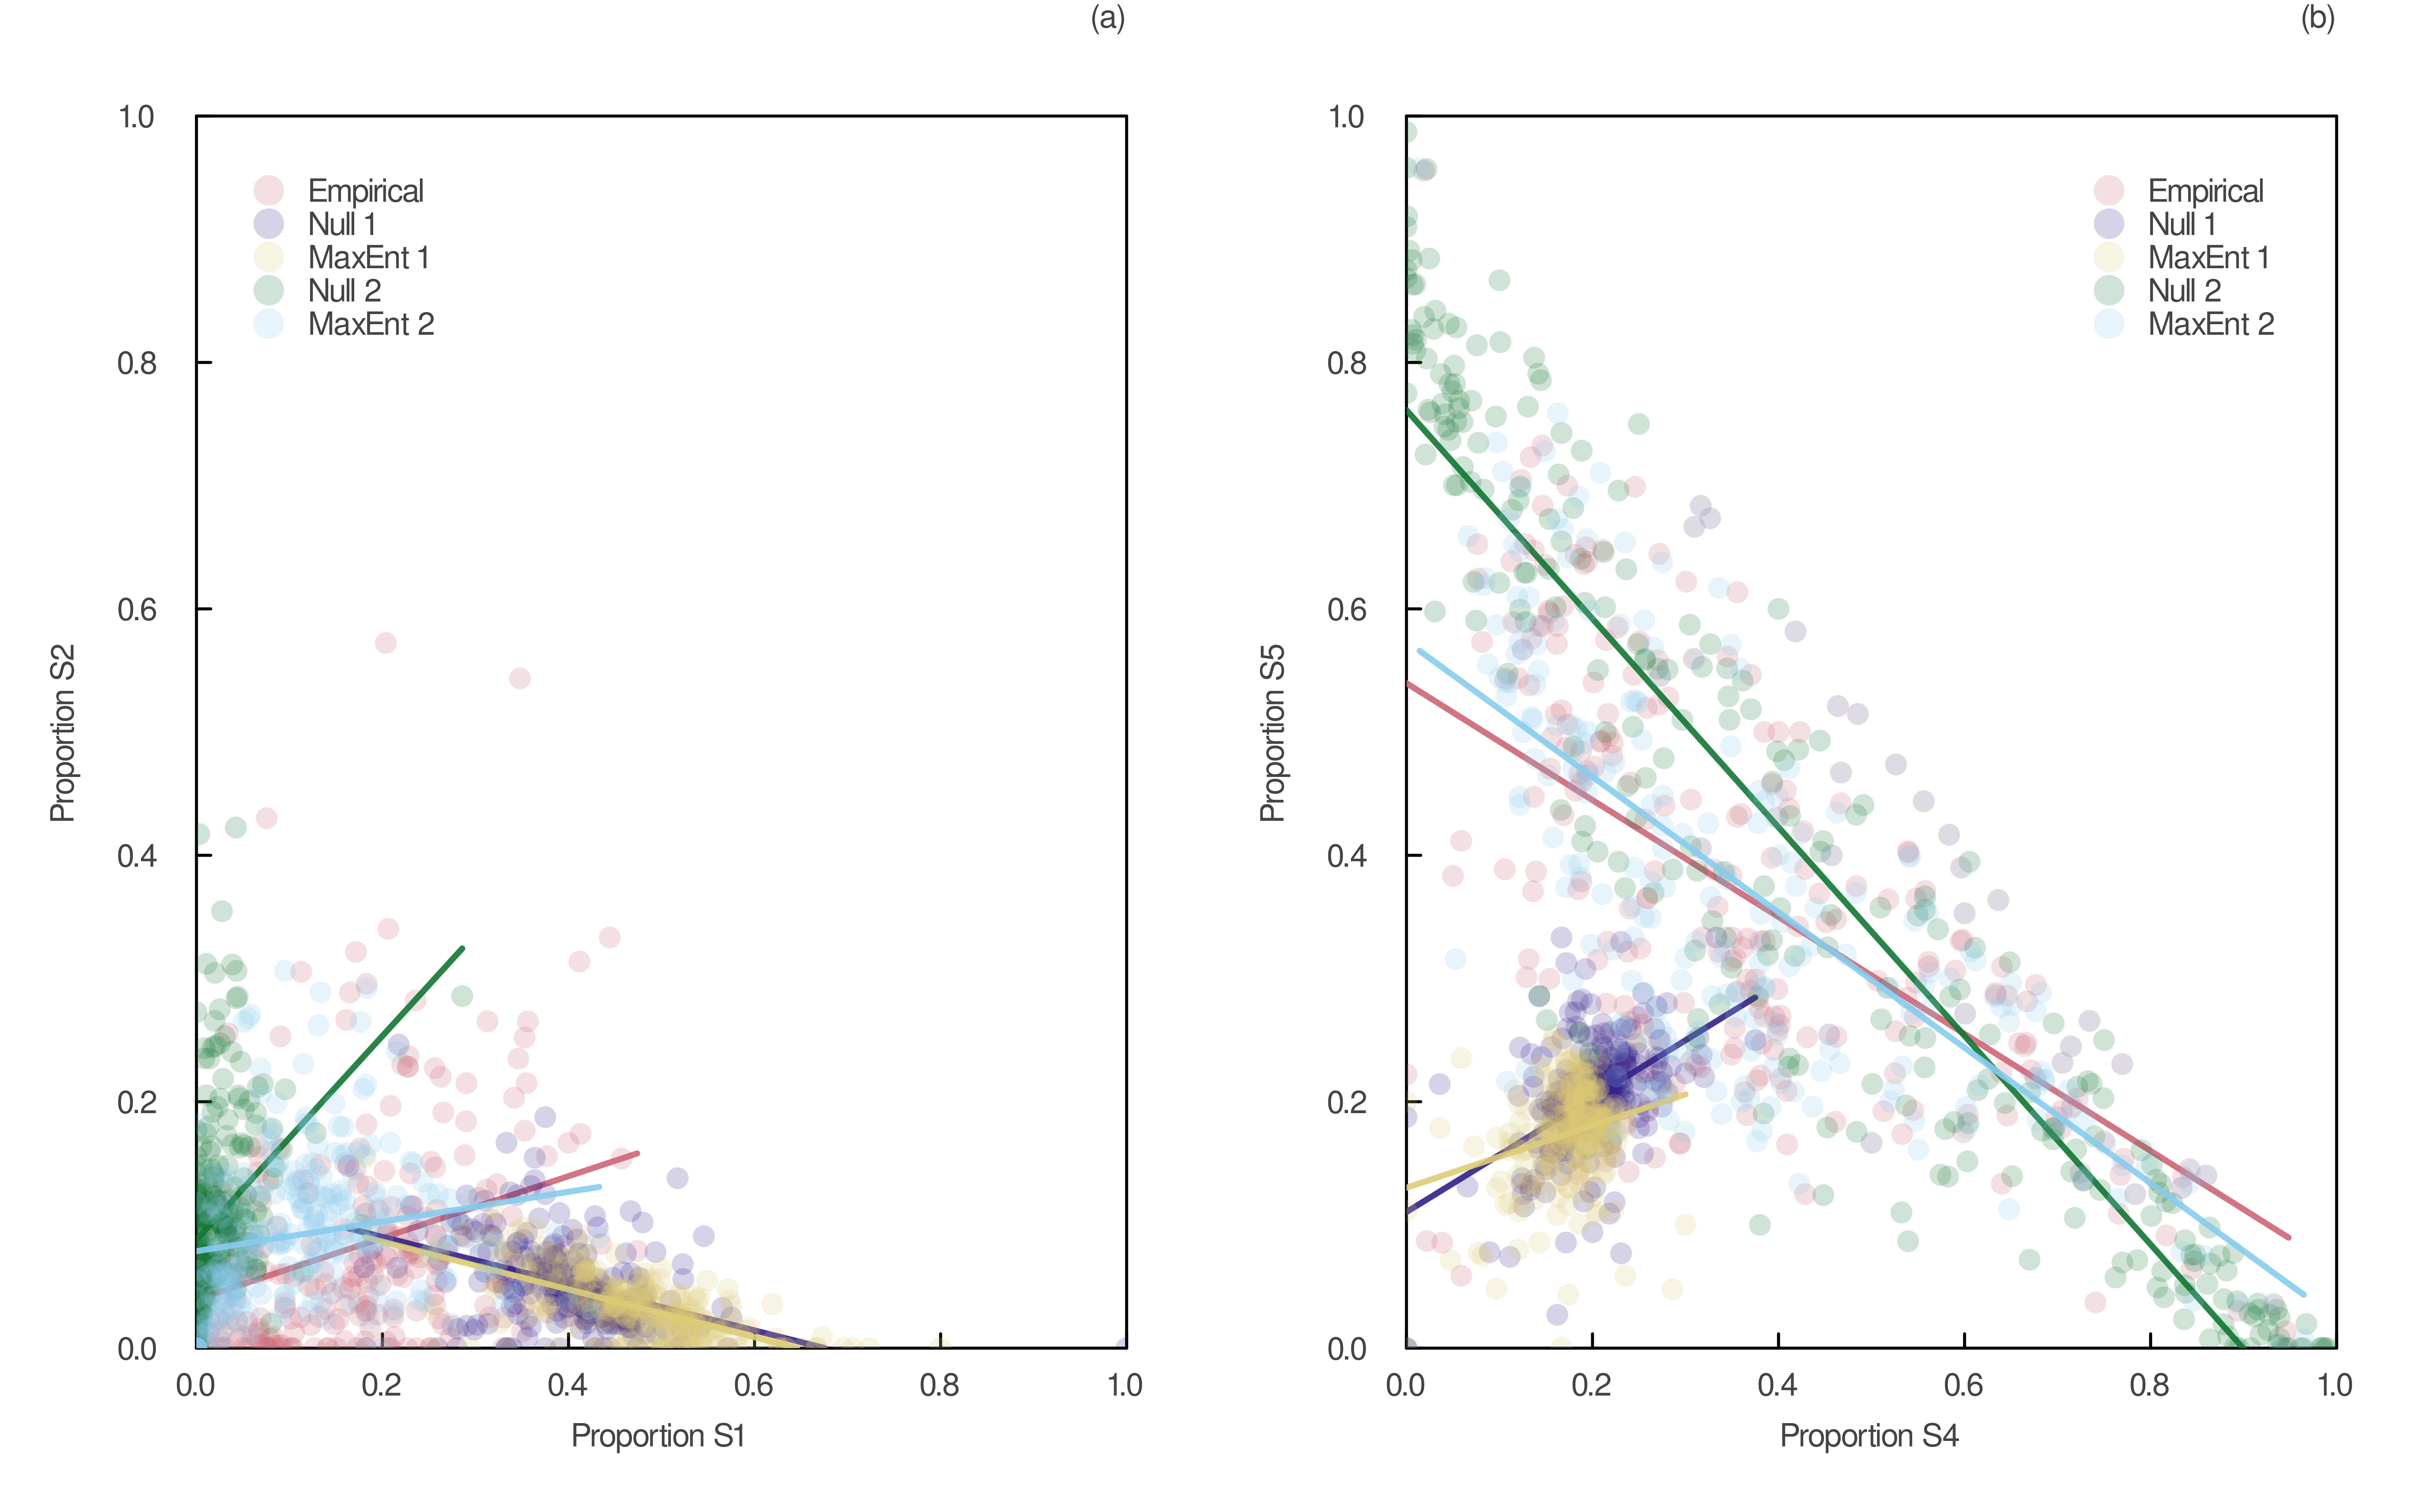
\includegraphics[width=\textwidth]{figures/article2/motifs_relations.png}
  \caption{\textbf{Pairwise relationships between the proportions of single-link three-species motifs in empirical and predicted food webs.}
    S1: Tri-trophic chain. S2: Omnivory. S4: Apparent competition. S5:
    Exploitative competition. Null 1: Type I null model based on connectance.
    MaxEnt 1: Type I heuristic MaxEnt model based on connectance. Null 2: Type
    II null model based on the joint degree sequence. MaxEnt 2: Type II
    heuristic MaxEnt model based on the joint degree sequence. Regression lines
    are plotted in each panel. Motif S3 is not shown because of its low
    proportion in most empirical and predicted networks.}
  \label{fig:motifs_rel}
\end{figure}

}

One of the challenges in implementing and validating a maximum entropy model is
to discover where its predictions break down. The results depicted in
Table~\ref{tbl:measures_all} and Figure~\ref{fig:measures} show that our type II heuristic
MaxEnt model can capture many high-level properties of food webs, but does a
poor job of capturing others. This suggests that, although the joint degree
sequence is an important driver of food-web structure, other ecological
constraints might be needed to account for some emerging food-web properties,
especially the ones regarding food-chain lengths. Nevertheless,
Figures~\ref{fig:motifs} and \ref{fig:motifs_rel} show that this model can reproduce
surprisingly well motif profiles, one of the most ecologically informative
properties of food webs. This suggests that the emerging structure of food webs
is mainly driven by their joint degree sequence, although higher-level
properties might need to be included in the model to ensure that food-chain
lengths fall within realistic values. 


\section{Conclusion}

The principle of maximum entropy is a mathematical method of finding
least-biased probability distributions that have some specified properties given
by prior knowledge about a system. We first applied this conventional MaxEnt
approach on food webs to predict species-level properties, namely the joint
degree distribution and the degree distribution of maximum entropy given known
numbers of species and interactions. We found that the joint degree
distributions of maximum entropy had a similar shape to the ones of empirical
food webs in high-connectance systems. However, these MaxEnt distributions were
more symmetric than the ones of empirical food webs when connectance was low,
which suggests that other constraints might be needed to improve these
predictions in low-connectance systems. Then, we used a slightly different
approach that aimed at finding heuristically the network configuration with the
highest SVD entropy, i.e. whose vector of relative singular values has maximum
entropy. This network of maximum entropy is the most complex, or random, given
the specified structure. We found that the heuristic maximum entropy model based
on connectance did not predict the structure of sampled food webs very well.
However, the heuristic maximum entropy model based on the entire joint degree
sequence, i.e. on the number of prey and predators for each species, gave more
convincing results. Indeed, this model reproduced food-web structure
surprisingly well, including the highly informative motif profile. Nevertheless,
it was not able to predict realistic food-chain lengths. 

Our results bring to the forefront the role of the joint degree distribution in
shaping food-web structure. This echoes the work of \textcite{Fortuna2010Nestedness},
who found that the degree distribution of ecological networks drives their
emerging structure such as their nestedness and modularity. Several measures of
food webs have been analyzed when studying the ecological consequences of
network structure (\cite{McCann2011Food}, \cite{Delmas2019Analysing}). In fact,
following \textcite{Williams2011Biology}, we believe that there is a lot more
ecological information in the deviation between these properties in empirical
systems and their maximum entropy configuration given a fixed joint degree
sequence.  

\subsection{Alternative MaxEnt models}

In this contribution, we used a method based on simulated annealing to find the
network configuration with the highest SVD entropy while fixing some aspects of
its structure. However, there are different ways to generate adjacency matrices
using MaxEnt. Another technique, also based on simulated annealing, could begin
by generating a food web randomly with fixed numbers of species and interactions
and calculating its joint degree distribution. Pairs of interactions could then
be swapped sequentially until we minimize the divergence between the calculated
joint degree distribution and the one of maximum entropy obtained analytically.
In that case, this is the entropy of the joint degree distribution that would be
maximized, not the one of the network's topology. To a certain extent, this
method would bridge the gap between the analytical and heuristic approaches
presented in this article. More research is needed to compare the quality of
different methods in generating adjacency matrices of food webs using MaxEnt.  

Maximum entropy graph models are another type of method that predicts a
distribution of adjacency matrices under soft or hard constraints (e.g.
\cite{Park2004Statistical}, \cite{Cimini2019Statistical}). Under hard
constraints, every network with a non-zero probability exactly satisfies the
constraints on its structure. This is in contrast with soft constraints, which
require that networks satisfy them on average (i.e. many networks with a
non-zero probability do not have the exact structure set by the constraints).
Maximum entropy graph models are helpful because they can provide probability
distributions for many network properties by measuring the structure of all
adjacency matrices with a non-zero probability. However, we consider that our
approach based on simulated annealing is more flexible and more computationally
efficient. Indeed, many measures of food-web structure are hard to translate
into mathematical constraints. Moreover, because food webs are directed networks
that can have self-loops, it makes the mathematical derivation of maximum
entropy graph models difficult. We believe that identifying heuristically what
constrains the topology of food webs is a useful first step before attempting to
derive the mathematical formulation of a maximum entropy graph model for food
webs. 

\subsection{Applications}

Our analytical and heuristic models can be applied for different purposes.
First, they could be used to generate first-order approximations of a network's
properties when state variables are known empirically. For example, knowing the
number of species in an ecological community, we can predict its number of
interactions using the flexible links model and then predict its joint degree
distribution with minimal biases using the principle of maximum entropy. This
could prove particularly useful when predicting network structure at large
spatial scales, subdividing the study area into smaller communities (e.g. grid
cells). Indeed, because species richness and other ecological data are
increasingly abundant (e.g. \cite{Dickinson2010Citizen}), validated MaxEnt models
can be used to respond to a wider range of macroecological questions regarding
food webs. 

Second, our analytical model can be used to generate informative priors in
Bayesian analyses of the structure of ecological networks (e.g.
\cite{Cirtwill2019Quantitative}). Indeed, the probability distribution of maximum
entropy derived using MaxEnt can be used as a prior that can be updated with
novel data. For instance, if we know the number of species and the number of
interactions, we can derive the degree distribution of maximum entropy, as shown
in this contribution. The degree distribution represents the probability that a
species can interact (as a predator or a prey) with a given number of other
species. Data on species interactions can be used to update the prior degree
distribution to generate a more accurate posterior distribution, thus improving
our description and understanding of the system.

Third, our analytical and heuristic models can be used to make better
predictions of pairwise species interactions by constraining the space of
feasible networks, as discussed in \textcite{Strydom2021Roadmapa}. In other words, we
can use the network configuration or specific measures of food-web structure
derived using MaxEnt to ensure that our predictions of interspecific
interactions form feasible networks. This means that the probability that two
species interact may be conditional on the network structure and the probability
of interactions of all other species pairs. When data are limited, MaxEnt can be
used to predict network structure on which pairwise probabilities of
interactions are conditional.

Finally, our analytical and heuristic models can be used as alternative null
models of ecological networks to better understand and identify the ecological
processes driving food-web structure. Indeed, these mechanisms can be better
described when analyzing the deviation of empirical data from MaxEnt predictions
(\cite{Caruso2022Fluctuating}). A strong deviation would indicate that ecological
mechanisms not captured by the statistical constraints are at play for the
system at hand. For instance, the incapacity of a MaxEnt model to reliably
predict entropy may be a compelling indication of additional constraints shaping
food-web structure. If deviations are systematic, the maximum entropy model
might need to be revised to include appropriate ecological constraints. This
revision process helps us reflect on and identify what constrains food-web
structure. However, it is important to note that tangible ecological mechanisms
cannot be directly inferred from statistical distributions
(\cite{WarrenII2022Seeing}). Instead, by identifying the constraints of a
system and by analyzing empirical deviations from maximum entropy predictions,
MaxEnt can only help us redirect research efforts toward understanding the
biological mechanisms behind these constraints. 

The principle of maximum entropy can thus be applied to both the prediction and
understanding of natural systems. The model's interpretation depends on how we
use it. It can be used as a baseline distribution to identify the ecological
processes organizing natural systems. It can also be used to generate
predictions of ecological networks. This distinction between understanding and
predicting is important when using and interpreting MaxEnt models. 

\subsection{Final remarks}

One of the biggest challenges in using the principle of maximum entropy is to
identify the set of state variables that best reproduce empirical data. We found
that the number of species and the number of interactions are important state
variables for the prediction of the joint degree distribution. Similarly, we
found that the numbers of prey and predators for each species in a food web are
important state variables for the prediction of the network configuration.
However, our predictions overestimated the symmetry of the joint degree
distribution for our analytical model and the maximum trophic level and network
diameter for our heuristic model. We should thus continue to play the ecological
detective to find these other topological constraints that would improve the
predictions of MaxEnt models and help us understand better what drives food-web
structure.

\section{Acknowledgments}

We acknowledge that this study was conducted on land within the traditional
unceded territory of the Saint Lawrence Iroquoian, Anishinabewaki, Mohawk,
Huron-Wendat, and Omàmiwininiwak nations. This work was supported by the
Institute for Data Valorization (IVADO, PhD-2019a-5993304626), which supported
FB, and the Natural Sciences and Engineering Research Council of Canada (NSERC)
Collaborative Research and Training Experience (CREATE) program, through the
Computational Biodiversity Science and Services (BIOS2) program, which supported
FB, DG, and TP. TP received funding from the Canadian Institute for Ecology and
Evolution and a donation from the Courtois Foundation. TP also acknowledges
financial support from NSERC through the Discovery Grants and Discovery
Accelerator Supplement programs. 

 % Pour générer la bibliographie à la fin
 % de l'article, utiliser la commande de la
 % classe <dms> \sectionbibliography{<nom du .bib>}.
 % Il y a aussi la possibilité d'utiliser le package
 % <chapterbib>, auquel cas on utilise simplement
 % \bibliography normalement.
 %
 % IMPORTANT : Dans tous les cas, il faut faire
 %    pdflatex these
 %    bibtex chapitre1
 %    bibtex chapitre2
 %    .
 %    .
 %    .
 %    bibtex chapitreN
 %    pdflatex these
 %    pdflatex these
 %
 % où <these> est le nom du .tex principal
 % (qui contient le \documentclass).
 % bibtex a besoin du .aux de chapitre1 et
 % non du .tex. Il est parfois nécessaire
 % d'effacer le .aux et de recommencer la
 % compilation du début.
%%\bibliographystyle{amsplain} % style plain anglais ou
%% \bibliographystyle{amsplain-french} % style plain francais
%%\bibliographystyle{<style>} % autre
%% \sectionbibliography{ref.bib} %Donner le nom du .bib

\endinput
%%
%% End of file `03_article2.tex'.


%%%%%%%%%%%%%%%%%%%%%%%%%%%%%%%%%%%%%%%%%%%%%%%%%%%%%%%%%%%%
%%%%%%%%%%%%%%%%%%%                     %%%%%%%%%%%%%%%%%%%%
%%%%%%%%%%%%%%%%%%% C O N C L U S I O N %%%%%%%%%%%%%%%%%%%%
%%%%%%%%%%%%%%%%%%%                     %%%%%%%%%%%%%%%%%%%%
%%%%%%%%%%%%%%%%%%%%%%%%%%%%%%%%%%%%%%%%%%%%%%%%%%%%%%%%%%%%
% %%
%% This is file `04_conclusion.tex',
%% generated with the docstrip utility.
%%

% Utilisez la macro de langue appropriée.
\francais   
%ou
%%\anglais

\chapter{Conclusions générales}

Cette thèse pose les fondements de la théorie de l'entropie maximale des réseaux
trophiques (Trophique-METE). Basée sur le principe d'entropie maximale, cette
théorie permet d'inférer des distributions de probabilité caractérisant la
structure émergente des réseaux trophiques. Les distributions prédites sont
celles qui représentent le mieux les informations fournies par les contraintes
écologiques, sans faire de supposition additionnelle sur la forme de la
distribution au-delà des contraintes choisies. Plusieurs versions de la théorie
peuvent être développées selon les contraintes utilisées et les distributions
prédites. Cette thèse développe et teste deux versions restreintes de la théorie
(Article~\ref{art:article2}). 

L'article~\ref{art:article1} constitue le cadre conceptuel de la théorie. Il
explique pourquoi les interactions entre espèces, telles que les interactions
prédateurs-proies et plantes-herbivores, sont intrinsèquement probabilistes.
Notre manque de connaissances sur les interactions locales et régionales, en
partie attribuable aux limites d'observation des interactions entre espèces
(\cite{Jordano2016Sampling}), ainsi que la variabilité spatiale et temporelle
des interactions locales (\cite{Poisot2015Species}), introduisent une
incertitude dans notre mesure des interactions. Cette incertitude est
irréductible à l'échelle locale, c.-à-d. qu'elle persiste même avec l'ajout de
nouvelles données empiriques. Cet article souligne l'importance d'identifier, de
quantifier et de communiquer cette incertitude inhérente aux interactions entre
espèces. 

Trophique-METE fournit un cadre d'analyse permettant de quantifier plus
facilement et avec cohérence l'incertitude au sein des réseaux trophiques à
partir d'un nombre limité d'informations écologiques. Elle s'inscrit donc dans
la vision probabiliste des réseaux élaborée dans l'article~\ref{art:article1} en
générant des prédictions probabilistes de différentes mesures de la structure
des réseaux trophiques. En effet, puisque l'incertitude des interactions entre
espèces se propage à la structure émergente des réseaux, cette dernière est
également probabiliste. En approfondissant notre compréhension des interactions
probabilistes, nous pouvons mieux interpréter les prédictions de la théorie
(comme la distribution jointe de degrés, qui décrit la probabilité qu'une espèce
ait un nombre donné de proies et de prédateurs). Les sources d'incertitude et
mécanismes écologiques sous-jacents aux interactions entre espèces, décrits dans
l'article~\ref{art:article1}, peuvent inspirer le développement de différentes
versions de la théorie, p. ex. en prenant comme variables d'état celles qui
conditionnent les probabilités d'interactions entre espèces. Puisque les
prédictions de Trophique-METE ne sont basées que sur ces variables d'état, cette
théorie infère la structure des réseaux sans supposer (à tort) que les
interactions entre espèces sont indépendantes les unes des autres, ce qui
contribue à la robustesse de la théorie.

En reconnaissant que la structure émergente des réseaux trophiques est
écologiquement et statistiquement contrainte, l'article~\ref{art:article2} jette
les bases de la théorie de l'entropie maximale des réseaux trophiques. Il montre
deux approches (analytique et heuristique) pour prédire la structure des réseaux
trophiques à l'aide du principe d'entropie maximale. L'approche analytique
permet d'inférer directement une distribution de probabilité à l'aide de la
méthode des multiplicateurs de Lagrange, alors que l'approche heuristique permet
d'identifier le réseau d'entropie (ou de complexité) maximale en permutant
aléatoirement les interactions entre espèces tout en respectant les contraintes
imposées par les variables d'état. Les deux versions de la théorie développées
dans cet article, qui diffèrent selon les variables d'état utilisées, mettent en
œuvre ces deux approches. Cet article fournit également les outils nécessaires
pour développer d'autres versions de la théorie reposant sur d'autres variables
d'état. Dans les sous-sections suivantes, je discute des développements actuels
et futurs, des tests à venir et des applications potentielles de la théorie. 

%% Développer la théorie

\section{Développement de la théorie de l'entropie maximale des réseaux trophiques} 

\subsection{Où en sommes-nous?} 

L'article~\ref{art:article2} propose deux premières versions de la théorie,
employant les approches analytiques et heuristiques basées sur le principe
d'entropie maximale. La première version de Trophique-METE prédit la structure
des réseaux trophiques à partir du nombre d'espèces et du nombre d'interactions.
Cette version a permis de prédire la distribution jointe de degrés (approche
analytique) et la matrice d'adjacence utilisée pour calculer différentes mesures
de la structure des réseaux (approche heuristique). La deuxième version, quant à
elle, prédit la matrice d'adjacence à partir du nombre de proies et de
prédateurs pour chaque espèce dans le réseau (approche heuristique). La première
version prédit bien la distribution jointe de degrés lorsque la connectance du
réseau est élevée, alors que la seconde version prédit mieux les autres mesures
testées (comme l'emboîtement et la proportion des motifs à trois espèces).
Cependant, ces deux versions surestiment systématiquement le niveau trophique
maximal et le diamètre des réseaux, ce qui suggère que les variables utilisées
ne capturent pas adéquatement certains mécanismes importants sous-jacents aux
réseaux, notamment en ce qui a trait au transfert d'énergie au sein des systèmes
écologiques complexes. Malgré cela, les réseaux trophiques empiriques sont
proches de leur entropie maximale tel que prédit par mes modèles, ce qui suggère
que les variables utilisées parviennent tout de même à bien capturer la
complexité des réseaux trophiques, et par conséquent, une grande partie des
mécanismes écologiques sous-jacents aux réseaux. 

\subsection{Comment améliorer et étendre la théorie?} 

Différentes versions de la théorie de l'entropie maximale des réseaux trophiques
peuvent être développées selon les variables d'état choisies. La sélection des
variables d'état peut se faire sur la base des limites et erreurs de prédiction
des versions précédentes. Par exemple, puisque les versions élaborées dans
l'article~\ref{art:article2} n'ont pas réussi à prédire adéquatement le niveau
trophique maximal et le diamètre des réseaux, une version contraignant la
longueur des chaînes trophiques pourrait s'avérer plus précise. Une telle
version pourrait utiliser l'énergie métabolique totale de la communauté comme
variable d'état (imposant une limite au transfert d'énergie au sein des réseaux)
ou le niveau trophique moyen comme contrainte écologique. Bien que le
développement de telles versions améliorées de la théorie puisse permette
d'obtenir de meilleures prédictions de la structure des réseaux trophiques,
elles se cantonnent à une seule représentation des réseaux (p. ex. aux réseaux
d'interactions entre espèces), sans tenir compte des différents niveaux
d'organisation et de mesure des interactions.

Pour être plus complète, une théorie élargie de l'entropie maximale des réseaux
trophiques devrait pouvoir prédire simultanément différentes représentations des
réseaux trophiques. Cette théorie élargie serait l'extension logique de la
théorie de l'entropie maximale de l'écologie (METE, \cite{Harte2011Maximum}) aux
réseaux trophiques (d'où l'appellation «~Trophique-METE~»). La version ASNE de
METE utilise la superficie $A_0$, le nombre d'espèces $S_0$, le nombre total
d'individus $N_0$ et l'énergie métabolique totale $E_0$ (ou la biomasse) d'une
communauté comme variables d'état pour prédire plusieurs distributions d'intérêt
en écologie (\cite{Harte2008Maximum}, \cite{Harte2011Maximum},
\cite{Harte2014Maximum}). Trophique-METE, dans sa version élargie, pourrait
notamment ajouter le nombre total d'interactions entre espèces $L_0$ à ces
variables d'état pour former la version ASNEL de la théorie. En plus des
prédictions macroécologiques de METE (telles que la relation aire-espèce et les
distributions du nombre d'individus et du taux métabolique par espèce), ASNEL
permettrait de prédire la relation entre la structure des réseaux et leur
superficie, tout en faisant le pont entre les réseaux d'interactions entre
individus et entre espèces. Cette théorie élargie permettrait ainsi d'avoir une
vision plus harmonieuse des réseaux trophiques représentés à différentes
échelles spatiales et taxonomiques.

Les versions élargies de Trophique-METE peuvent être construites autour de
plusieurs autres variables d'état pour tenir compte des conditions locales
mentionnées dans l'article~\ref{art:article1}. Par exemple, le temps $t_0$ (qui
peut correspondre, entre autres, à la durée d'échantillonnage ou au temps écoulé
depuis le début de la succession primaire) peut être ajouté aux variables
d'état, ce qui permettrait de prédire la relation entre la structure des réseaux
et leur durée. Le temps pourrait également être intégré dans une version
dynamique de la théorie en laissant les valeurs des variables d'état fluctuer au
fil du temps, tel qu'effectué par \textcite{Harte2021Dynamete} dans leur version
dynamique de METE. Par ailleurs, le nombre de genres ou de familles au sein
d'une communauté peut également être ajouté aux variables d'état pour dériver
davantage de propriétés liées au niveau taxonomique, comme la relation
aire-genre ou aire-famille (\cite{Harte2014Maximum}). Dans le même ordre
d'idées, le nombre total d'interactions entre individus, genres ou familles peut
être intégré à la théorie pour prédire plus précisément la structure des réseaux
à différentes échelles taxonomiques. Le nombre total d'interactions entre
individus (c.-à-d. le nombre total d'événements de prédation survenus au cours
d'une période de temps donné) peut également être utilisé pour prédire la
structure des réseaux d'interactions quantitatives (p. ex. pour dériver la
distribution de fréquences d'interactions par espèce). Le principal obstacle à
la construction d'une telle théorie élargie des réseaux trophiques est le manque
actuel de données empiriques nécessaires pour tester et valider différentes
versions de la théorie. Cependant, poursuivre activement le développement de
Trophique-METE nous permet de mieux identifier les données et variables d'état à
échantillonner. 

Les prédictions de Trophique-METE sont intrinsèquement probabilistes. Cependant,
la matrice d'adjacence prédite pour un réseau particulier, avec la méthode
présentée dans l'article~\ref{art:article2}, est unique et composée
d'interactions binaires. Cela est dû à l'approche heuristique employée, qui
maximise l'entropie de la distribution des valeurs singulières au sein de la
matrice, permettant ainsi d'identifier celle ayant la plus grande complexité
interne. Trophique-METE peut également être développée pour inférer
analytiquement des distributions d'entropie maximale \textit{sur} les réseaux
(c.-à-d. générant des réseaux probabilistes tels que définis dans
l'article~\ref{art:article1}). Ces distributions peuvent être obtenues en
utilisant des contraintes rigides (où chaque réseau ayant une probabilité non
nulle satisfait exactement les contraintes) ou souples (où les réseaux prédits
satisfont les contraintes en moyenne). Mesurer la structure des réseaux à partir
de ces distributions d'entropie maximale nous permettrait de générer des
prédictions probabilistes pour l'ensemble des propriétés des réseaux. Le
développement de Trophique-METE autour des réseaux probabilistes constitue une
avancée naturelle dans la théorie, nous permettant d'aller au-delà des
prédictions uniques des réseaux, tout en offrant une alternative à l'évaluation
indépendante des probabilités d'interaction au sein des réseaux.  

%% Tester la théorie

\section{Validation de la théorie} 

\subsection{Quels réseaux sont d'entropie maximale?} 

\subsection{Un réseau d'entropie maximale est-il à l'équilibre?} 


%% Appliquer la théorie

\section{Applications potentielles de la théorie} 

\subsection{Compréhension des mécanismes sous-jacents aux réseaux d'interactions} 

\subsection{Prévision de la structure des réseaux trophiques} 


\endinput
%%
%% End of file `04_conclusion.tex'.


% S'il y a une bibliographie pour tout le document, on peut
% utiliser les commandes suivantes. À noter que le style est
% laisser au choix de l'auteur·e. (Il est même possible
% d'utiliser <natbib>).
% Il est possible d'avoir une bibliographie pour chaque
% chapitre. Consulter l'article en exemple pour voir
% comment faire.

\printbibliography

% Pour les annexes :
\appendix
% Les annexes se font comme les chapitres. Le fichier
% commence par \francais ou \anglais et ensuite
% \chapter{..}. Le reste est parreil à un chapitre normal.
%%%%%%%%%%%%%%%%%%%%%%%%%%%%%%%%%%%%%%%%%%%%%%%%%%%%%%%%%%%%
%%%%%%%%%%%%%%%%%%%%                   %%%%%%%%%%%%%%%%%%%%%
%%%%%%%%%%%%%%%%%%%%   A N N E X E S   %%%%%%%%%%%%%%%%%%%%%
%%%%%%%%%%%%%%%%%%%%                   %%%%%%%%%%%%%%%%%%%%%
%%%%%%%%%%%%%%%%%%%%%%%%%%%%%%%%%%%%%%%%%%%%%%%%%%%%%%%%%%%%
% %%
%% This is file `S_article1.tex',
%% generated with the docstrip utility.

%% Utilisez la macro de langue appropriée.\francais   
%ou
%% \anglais

\chapter{Matériel supplémentaire du premier article}\label{supp:A}


\begin{refsection}

\addtocontents{toc}{\protect\setcounter{tocdepth}{0}}

\section{Host-parasite network data}

\subsection{Data description}

We use the collection of tripartite host-parasite networks sampled across Europe
of \textcite{Kopelke2017Foodweb}. This dataset contains well-resolved binary local
interactions between willows ($52$ species), willow-galling sawflies ($96$
species), and their parasitoids ($126$ species). Out of a total of $374$ local
networks, we retained those containing at least $5$ species, resulting in a set
of $233$ georeferenced local networks (networks sampled within areas of $0.1$ to
$0.3$ km² during June and/or July spanning $29$ years). Given its replicated
networks spanning large spatiotemporal scales, this dataset is well-suited for
analyzing network variability.

We built a metaweb of binary interactions by aggregating all local interactions,
which gave us a regional network composed of $274$ species and $1080$
interactions. 

\subsection{Metawebs of probabilistic interactions}

We converted these binary regional interactions into probabilistic ones using
simple assumptions. Our aim is not to estimate precise probability values, but
to create plausible metawebs of probabilistic interactions for our illustrative
examples. 

We created two metawebs of probabilistic interactions by employing constant
false positive and false negative rates for all regional interactions. In the
first metaweb, we set both false positive and false negative rates to zero to
prevent artificially inflating the total number of interactions, enabling a more
accurate comparison with binary interaction networks. This gave us a probability
of regional interaction of $1$ when at least one interaction has been observed
locally and of $0$ in the absence of any observed interaction between a given
pair of species. This metaweb was used in Box~\ref{box2.2}. 

In the second metaweb, we introduced a $5\%$ false positive rate to account for
spurious interactions and a $10\%$ false negative rate to address the elevated
occurrence of missing interactions in ecological networks
(\cite{Catchen2023Missinga}). We believe these rates represent reasonable
estimates of missing and spurious potential interactions, but confirming their
accuracy is challenging due to the unavailability of data on the actual
feasibility of interactions. Observed interactions were thus given a probability
of regional interaction of $95\%$, whereas unobserved ones were assigned a
probability of $10\%$. This metaweb was used in Boxes~\ref{box2.3} and
\ref{box2.5}.

\subsection{Local networks of probabilistic interactions}

We built local networks of probabilistic interactions using the taxa found in
the empirical local networks and attributing pairwise interaction probabilities
based on the metawebs of probabilistic interactions $P(M_{i, j})$ (short for
$P(M_{i, j} = 1)$) and a constant value of $P(L_{i, j, k}|M_{i, j})$ (short for
$P(L_{i, j, k} = 1|M_{i, j} = 1)$) across interactions:

\begin{eqnarray}
    \label{eq:local_meta_sup}
    P(L_{i, j, k}) = P(L_{i, j, k} | M_{i, j})
    \times P(M_{i, j}).
\end{eqnarray}

We set all values of $P(L_{i, j, k}|M_{i, j})$ to $0.5$, $0.75$, or $1.0$
depending on the simulation. Intermediate values of $P(L_{i, j, k}|M_{i, j})$
around $50\%$ indicate considerable spatiotemporal variability, while higher
values close to $100\%$ indicate that regional interactions are nearly always
realized locally. 

\section{Additional methods for Box~\ref{box2.2}: Dissimilarity of local host-parasite networks}

\subsection{Dissimilarity between local networks and the metaweb}

We aggregated local networks of binary interactions by sequentially and randomly
selecting a number of local networks and aggregating both their species and
interactions. 

We compared the metaweb of binary interactions and the aggregated local networks
of binary interactions using the dissimilarity in species composition
$\beta_{S}$, and the dissimilarity of interactions between common species
$\beta_{OS}$ indices. Both dissimilarity indices were calculated based on the
number of items shared by the two networks ($c_{LM}$) and the number of items
unique to the metaweb ($u_M$) and the aggregated local network ($u_L$). The
$\beta_{S}$ dissimilarity index uses species (nodes) as items being compared,
while the $\beta_{OS}$ index assesses dissimilarity based on interactions
between shared species. Both indices were calculated following the $\beta_W$
index of \textcite{Whittaker1960Vegetation}: 

\begin{eqnarray}
    \label{eq:betadiv_network}
    \beta_W = \frac{c_{LM} + u_L + u_M}{(2 c_{LM} + u_L + u_M) / 2} - 1.
\end{eqnarray}

We repeated the aggregation process one hundred times and highlighted the median
dissimilarity values across simulations, as well as the $50\%$ and $95\%$
percentile intervals. 

\subsection{Aggregation of local networks of probabilistic interactions}

We aggregated local networks of probabilistic interactions similarly to the
networks of binary interactions, with the distinction that we also adjusted the
value of $P(L_{i, j, k})$ (short for $P(L_{i, j, k} = 1)$) when sampling
networks. The constancy of the probability of regional interaction across the
entire study area means that any rise in the probability of local interaction is
solely attributable to an increase in $P(L_{i, j, k}|M_{i, j})$. We adjusted the
value of $P(L_{i, j, k}|M_{i, j})$ as follows. Let $L_1$ and $L_2$ be two local
networks and $L_{1,2}$ the aggregated network. If $P(L_{i, j, 1}|M_{i, j})$ and
$P(L_{i, j, 2}|M_{i, j})$ are the probabilities that two potentially interacting
taxa interact respectively in $L_1$ and $L_2$, the probability $P(L_{i, j,
1,2}|M_{i, j})$ that these taxa interact in the aggregated network $L_{1,2}$ is
obtained by: 

\begin{eqnarray}
    \label{eq:aggregate}
    P(L_{i, j, 1, 2}|M_{i, j}) = 1 - [1 - P(L_{i, j, 1}|M_{i, j})] \times [1 -
P(L_{i, j, 2}|M_{i, j})],
\end{eqnarray}

assuming independence between the interaction of the two taxa in different
networks. This equation represents the probability that the interaction is
realized in either (1) exclusively the local network $L_1$, (2) exclusively the
local network $L_2$ or (3) both, given that the two taxa have the biological
capacity to interact. 

We then calculated the probabilities of local interaction of the aggregated
networks using Eq~\ref{eq:local_meta_sup}. The value of $P(L_{i, j, k}|M_{i,
j})$ for each curve in Figure~\ref{fig:accumulation}c-d is the probability before
aggregating networks.  

\subsection{Calculation of the expected number of local interactions and connectance}

We investigated how the number of local interactions and connectance scale with
the number of sampled (aggregated) local networks. We calculated the expected
numbers of interactions by taking the sum of all binary or probabilistic
interaction values. Connectance was calculated as the ratio of the expected
number of interactions to the number of possible (non-forbidden) interactions.
Because our networks are tripartite, connectance was calculated as follows: 

\begin{eqnarray}
    \label{eq:co_tri}
    Co = \frac{I}{S_S S_G + S_G S_P},
\end{eqnarray}

where $I$ is the expected number of interactions, $S_S$ the number of Salix
species, $S_G$ the number of galler species, and $S_P$ the number of parasitoid
species in the network. 

\section{Additional methods for Box~\ref{box2.3}: Spatial and temporal scaling of interactions}

\subsection{Aggregation of local and regional networks of probabilistic interactions} 

Local probabilistic interactions were derived from probabilistic regional
interactions by setting the value of $P(L_{i, j, k}|M_{i,j})$ (the local
probability of interaction among potentially interacting species) to $1$,
ensuring a conservative comparison between aggregated local networks and
metawebs. Aggregated local and regional networks were obtained by aggregating
both the species and interactions found within a particular latitudinal window.
The values of $P(L_{i, j, k}|M_{i, j})$ in local networks remained at their
maximum value of $1$ following Eq~\ref{eq:aggregate}. Latitudinal windows had
different positions (central latitudes) and widths (latitudinal widths).

\subsection{Calculation of the expected number of interactions}

We calculated the expected number of local and regional interactions by taking
the sum of all probabilistic interaction values of the aggregated networks. 

\section{Additional methods for Box~\ref{box2.5}: Sampling for binary interaction networks}

\subsection{Sampling using regional interaction probabilities}

We sampled for binary interaction networks across space, predicting a binary
interaction network for each location in our dataset. We performed a single
Bernoulli trial for each pair of taxa based on their regional probability of
interaction: 

\begin{eqnarray}
    \label{eq:sampling1}
    M_{i, j} \sim {\rm Bernoulli}(\phi_{i,j}),
  \end{eqnarray}
  
where $\phi_{i,j} = P(M_{i, j} = 1)$.

Every pair of taxa predicted to interact in this metaweb was treated as
interacting in all localized networks where they co-occurred, i.e. $L_{i, j, k}
= M_{i, j}$ when $X_{i,j,k} = 1$.

We performed between $1$ and $100$ simulations for each location to get a
distribution of networks of binary interactions sampled using regional
interaction probabilities.

\subsection{Sampling using local interaction probabilities}

We sampled binary interaction networks across space, predicting a binary
interaction network for each location in our dataset. We first generated
distinct probabilistic interaction networks for each location. The local
probability of interaction between potentially interacting species was set to
three different values: $P(L_{i, j, k}|M_{i, j}) = 1.0$, $P(L_{i, j, k}|M_{i,
j}) = 0.75$, and $P(L_{i, j, k}|M_{i, j}) = 0.50$. We then sampled each local
network of probabilistic interactions independently: 

\begin{eqnarray}
    \label{eq:sampling2}
    L_{i, j, k} \sim {\rm Bernoulli}(\phi_{i,j,k}),
  \end{eqnarray}
  
where $\phi_{i,j,k} = P(L_{i, j, k} = 1)$.

We performed between $1$ and $100$ simulations for each location to get a
distribution of networks of binary interactions sampled using local interaction
probabilities. 

\subsection{Calculation of connectance}

We calculated the connectance of our predicted tripartite networks of binary
interactions following Eq~\ref{eq:co_tri}. We calculated the average connectance
across simulations for each location.

\subsection{Calculation of the mean squared logarithmic error (MSLE)}

The mean squared logarithmic error was calculated as follows: 

\begin{eqnarray}
    \label{eq:MSLE_sup}
    MSLE = \frac{\sum (log(\overline{Co_L}) - log(\overline{Co_M}))^2}{n},
\end{eqnarray}

where $\overline{Co_L}$ and $\overline{Co_M}$ are the average connectance across
simulations for each location, respectively for local and regional samples, and
$n$ is the number of locations.

\clearpage

\addtocontents{toc}{\protect\setcounter{tocdepth}{-1}}

\begingroup
\let\cleardoublepage\clearpage
\printbibliography
\endgroup
\end{refsection}

\addtocontents{toc}{\protect\setcounter{tocdepth}{0}}

\endinput
%%
%% End of file `S_article1.tex'.
% %%
%% This is file `S_article2.tex',
%% generated with the docstrip utility.

%% Utilisez la macro de langue appropriée.
\francais   
%ou
%%\anglais

\chapter*{Appendix B. Supplementary material for \autoref{chapter2}}

\begin{figure}[h]
    \centering
    \includegraphics[width=\textwidth]{figures/S_article2/kin_kout_difference_strata.png}
    \caption{\textbf{Prediction errors of the absolute number of predators $k_{in}$ and prey
    $k_{out}$.} Species were ordered according to their total degree in their
    network. Networks were sorted into different groups based on their total number
    of species. In each panel, each dot corresponds to a single species within one
    of the networks whose total species count is within the specified range. The
    predicted joint degree sequences were obtained after sampling one realization of
    the joint degree distribution of maximum entropy for each network while keeping
    the total number of interactions
    constant.}
    \label{fig:kin_kout_diff_strata}
\end{figure}

\begin{figure}[h]
    \centering
    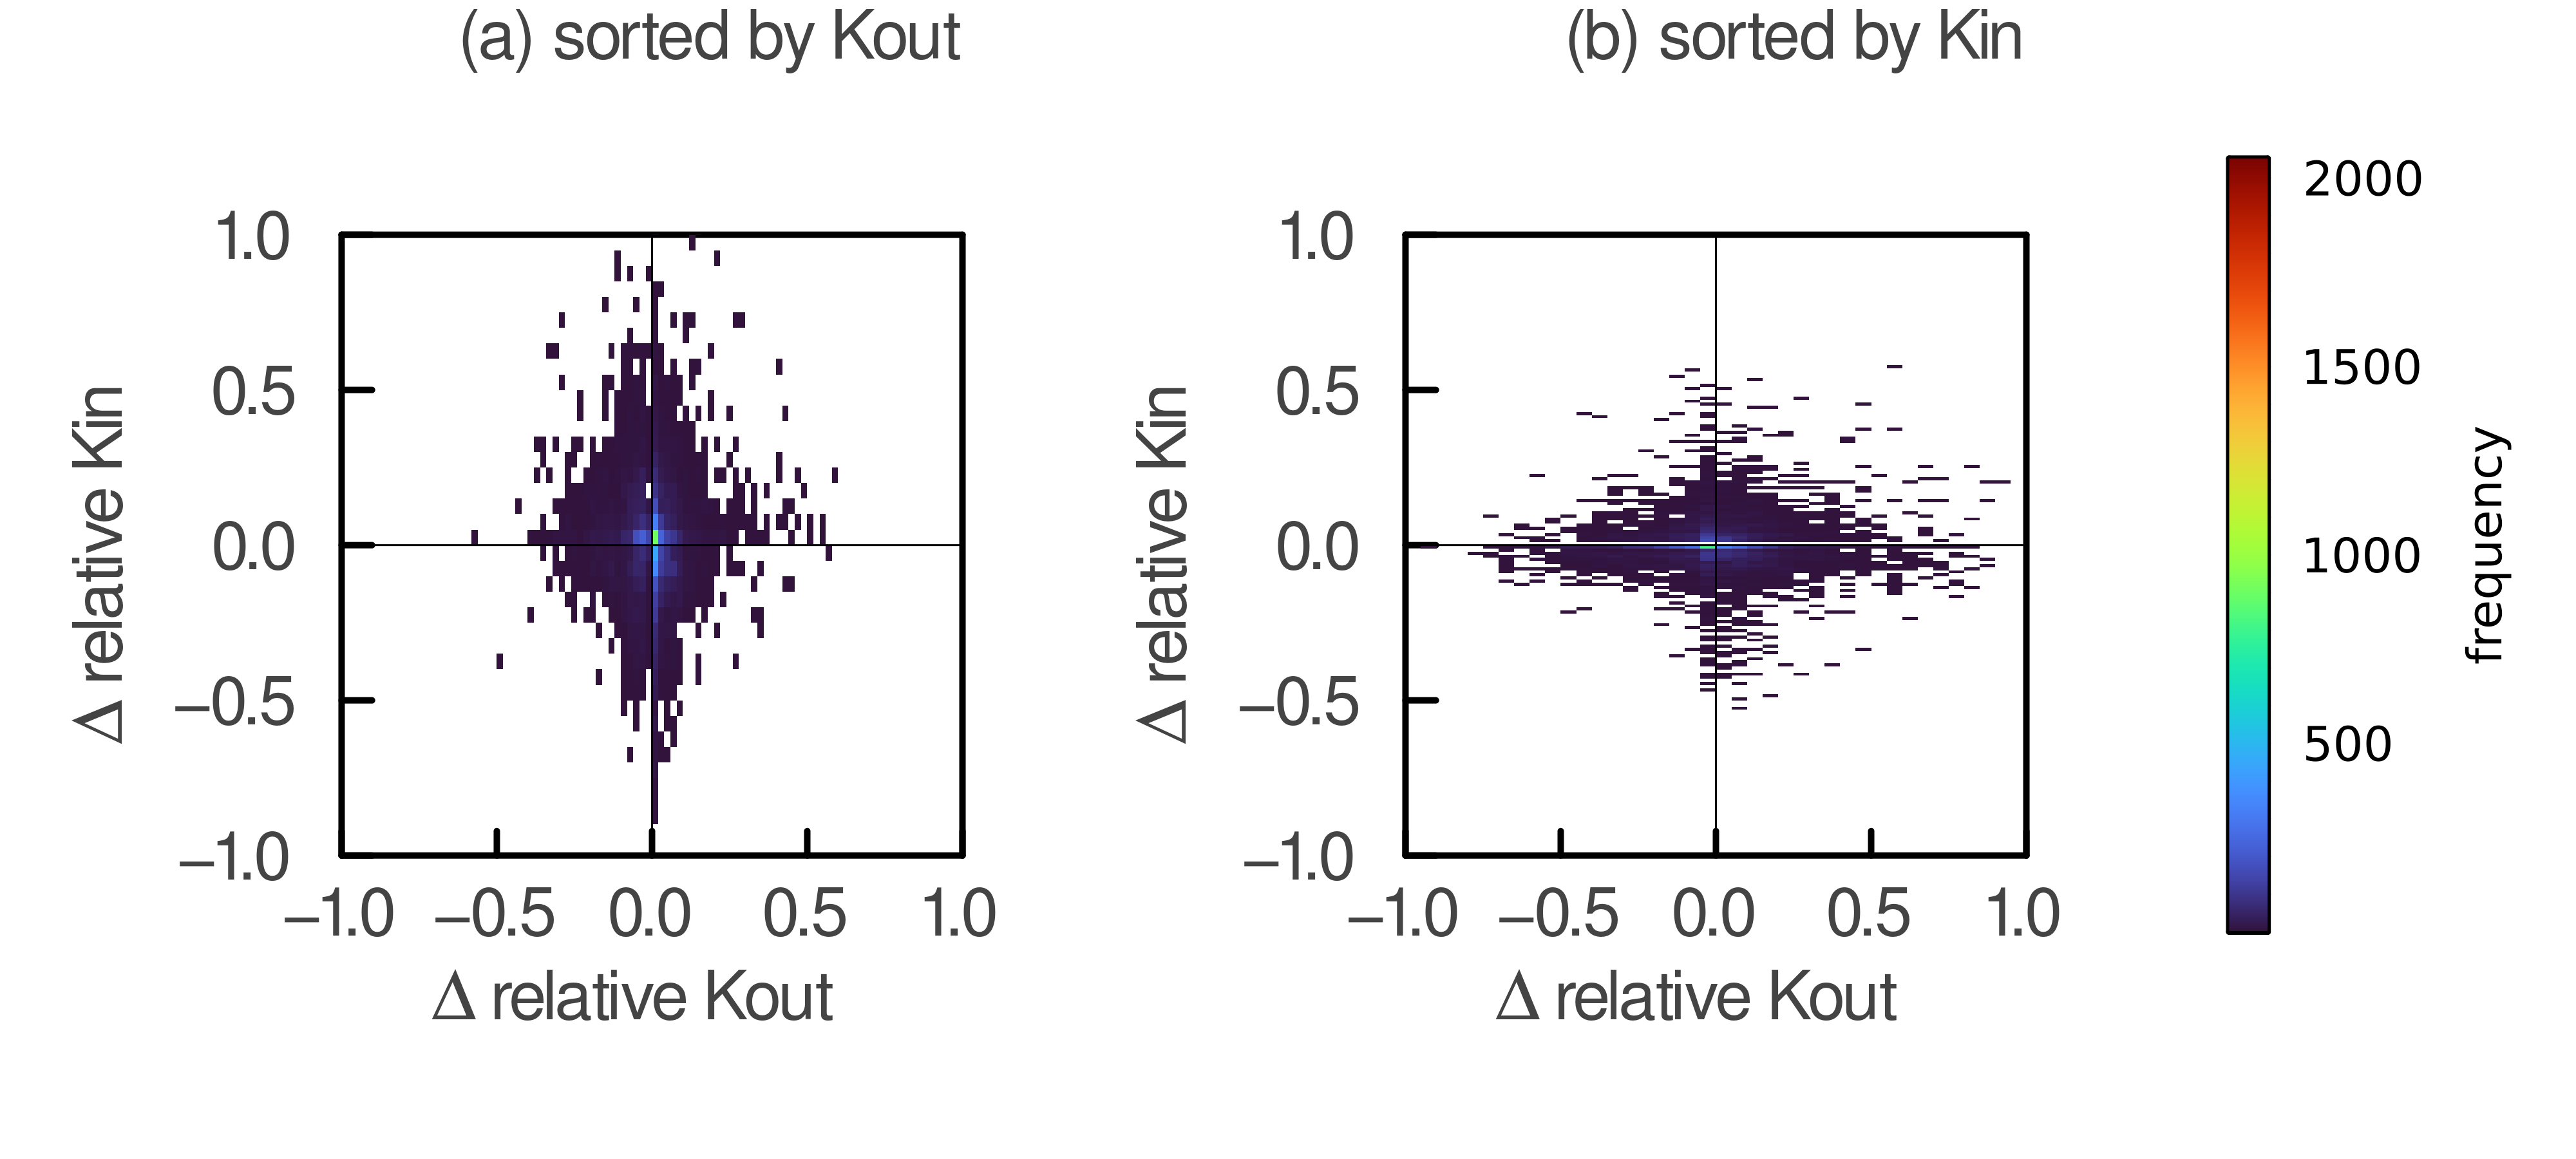
\includegraphics[width=\textwidth]{figures/S_article2/kin_kout_difference.png}
    \caption{\textbf{Prediction errors of the relative number of predators $k_{in}$ and prey
    $k_{out}$.} Species were ordered according to (a) their out-degree and (b)
    their in-degree. The predicted joint degree sequences were obtained after
    sampling one realization of the joint degree distribution of maximum entropy for
    each network while keeping the total number of interactions constant. Due to
    significant data overlap, all relationships are represented as 2D histograms.
    The color bar indicates the number of species that fall within each
    bin.}
    \label{fig:kin_kout_diff}
\end{figure}

\begin{figure}[h]
    \centering
    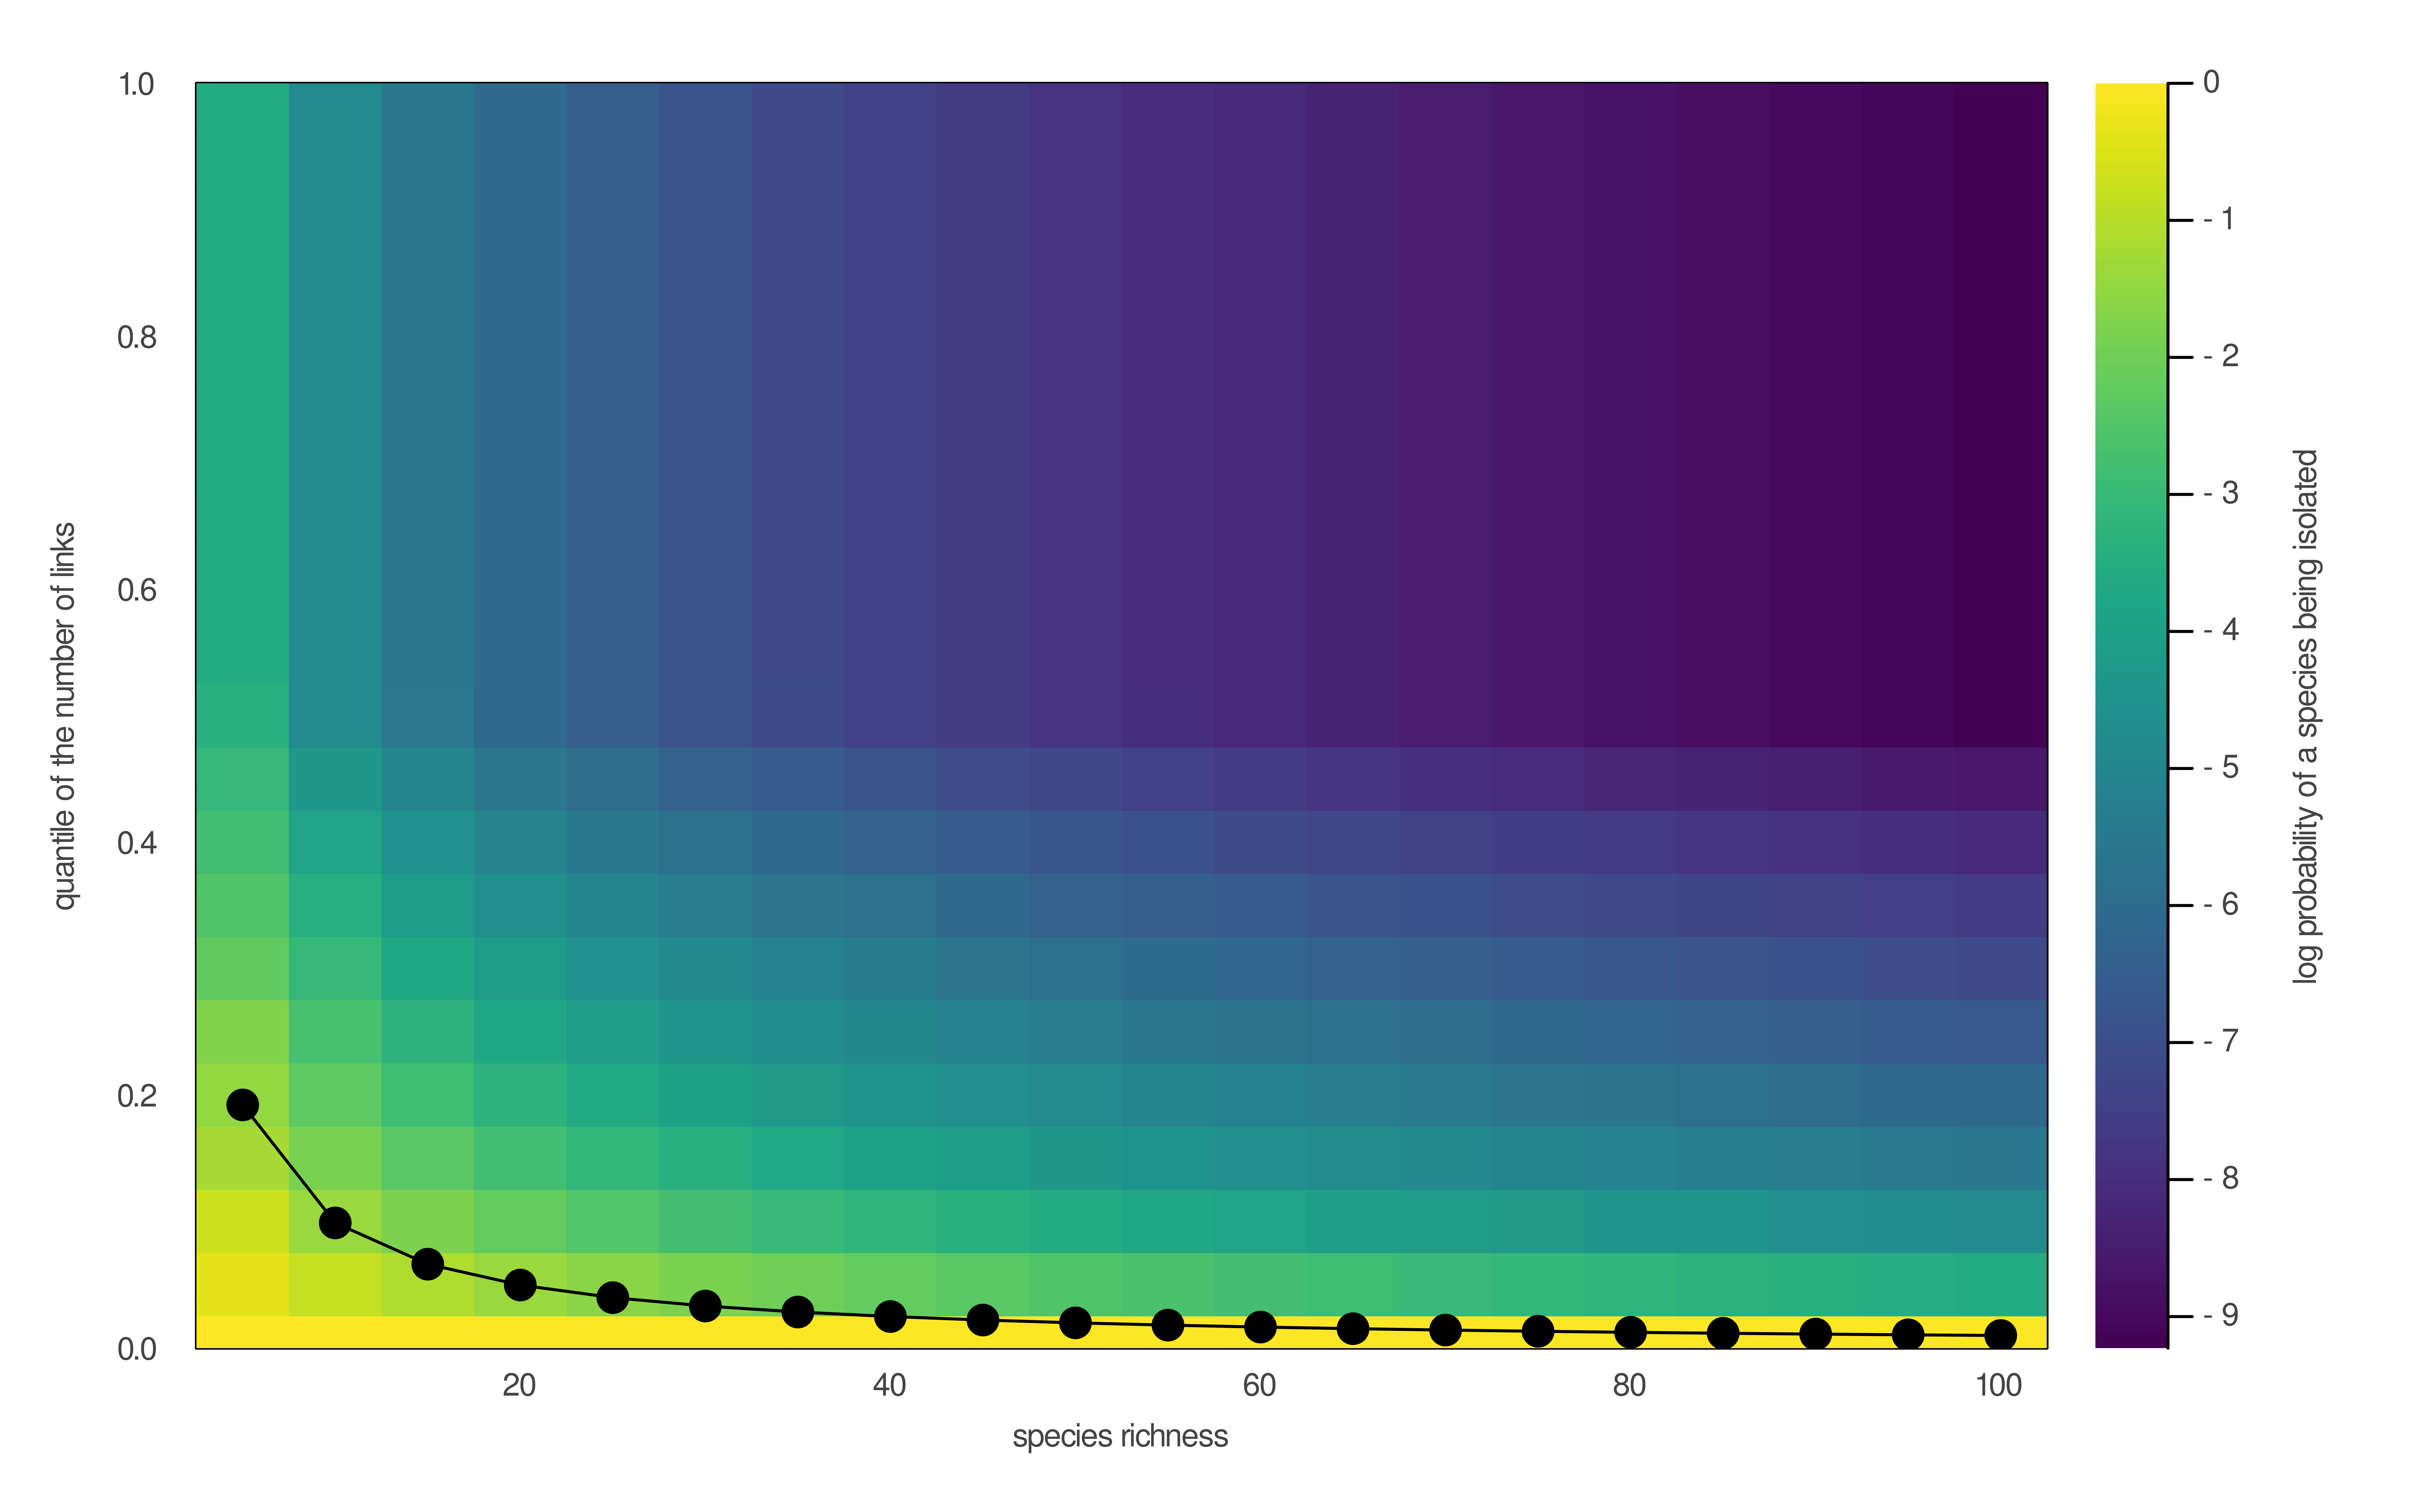
\includegraphics[width=\textwidth]{figures/S_article2/heatmap_disconnected.png}
    \caption{\textbf{Predicted probability that a species is isolated in its food web.} We
    derived many degree distributions of maximum entropy given a range of values of
    $S$ and $L$ and plotted the probability that a species has a degree $k$ of $0$
    (log-scale color bar). Species richness varies between $5$ and $100$ species, by
    increment of $5$ species. For each level of species richness, the numbers of
    interactions correspond to all 20-quantiles of the interval between $0$ and
    $S^2$. The black line marks the $S-1$ minimum number of interactions required to
    have no isolated species.}
    \label{fig:heatmap}
\end{figure}

\begin{figure}[h]
    \centering
    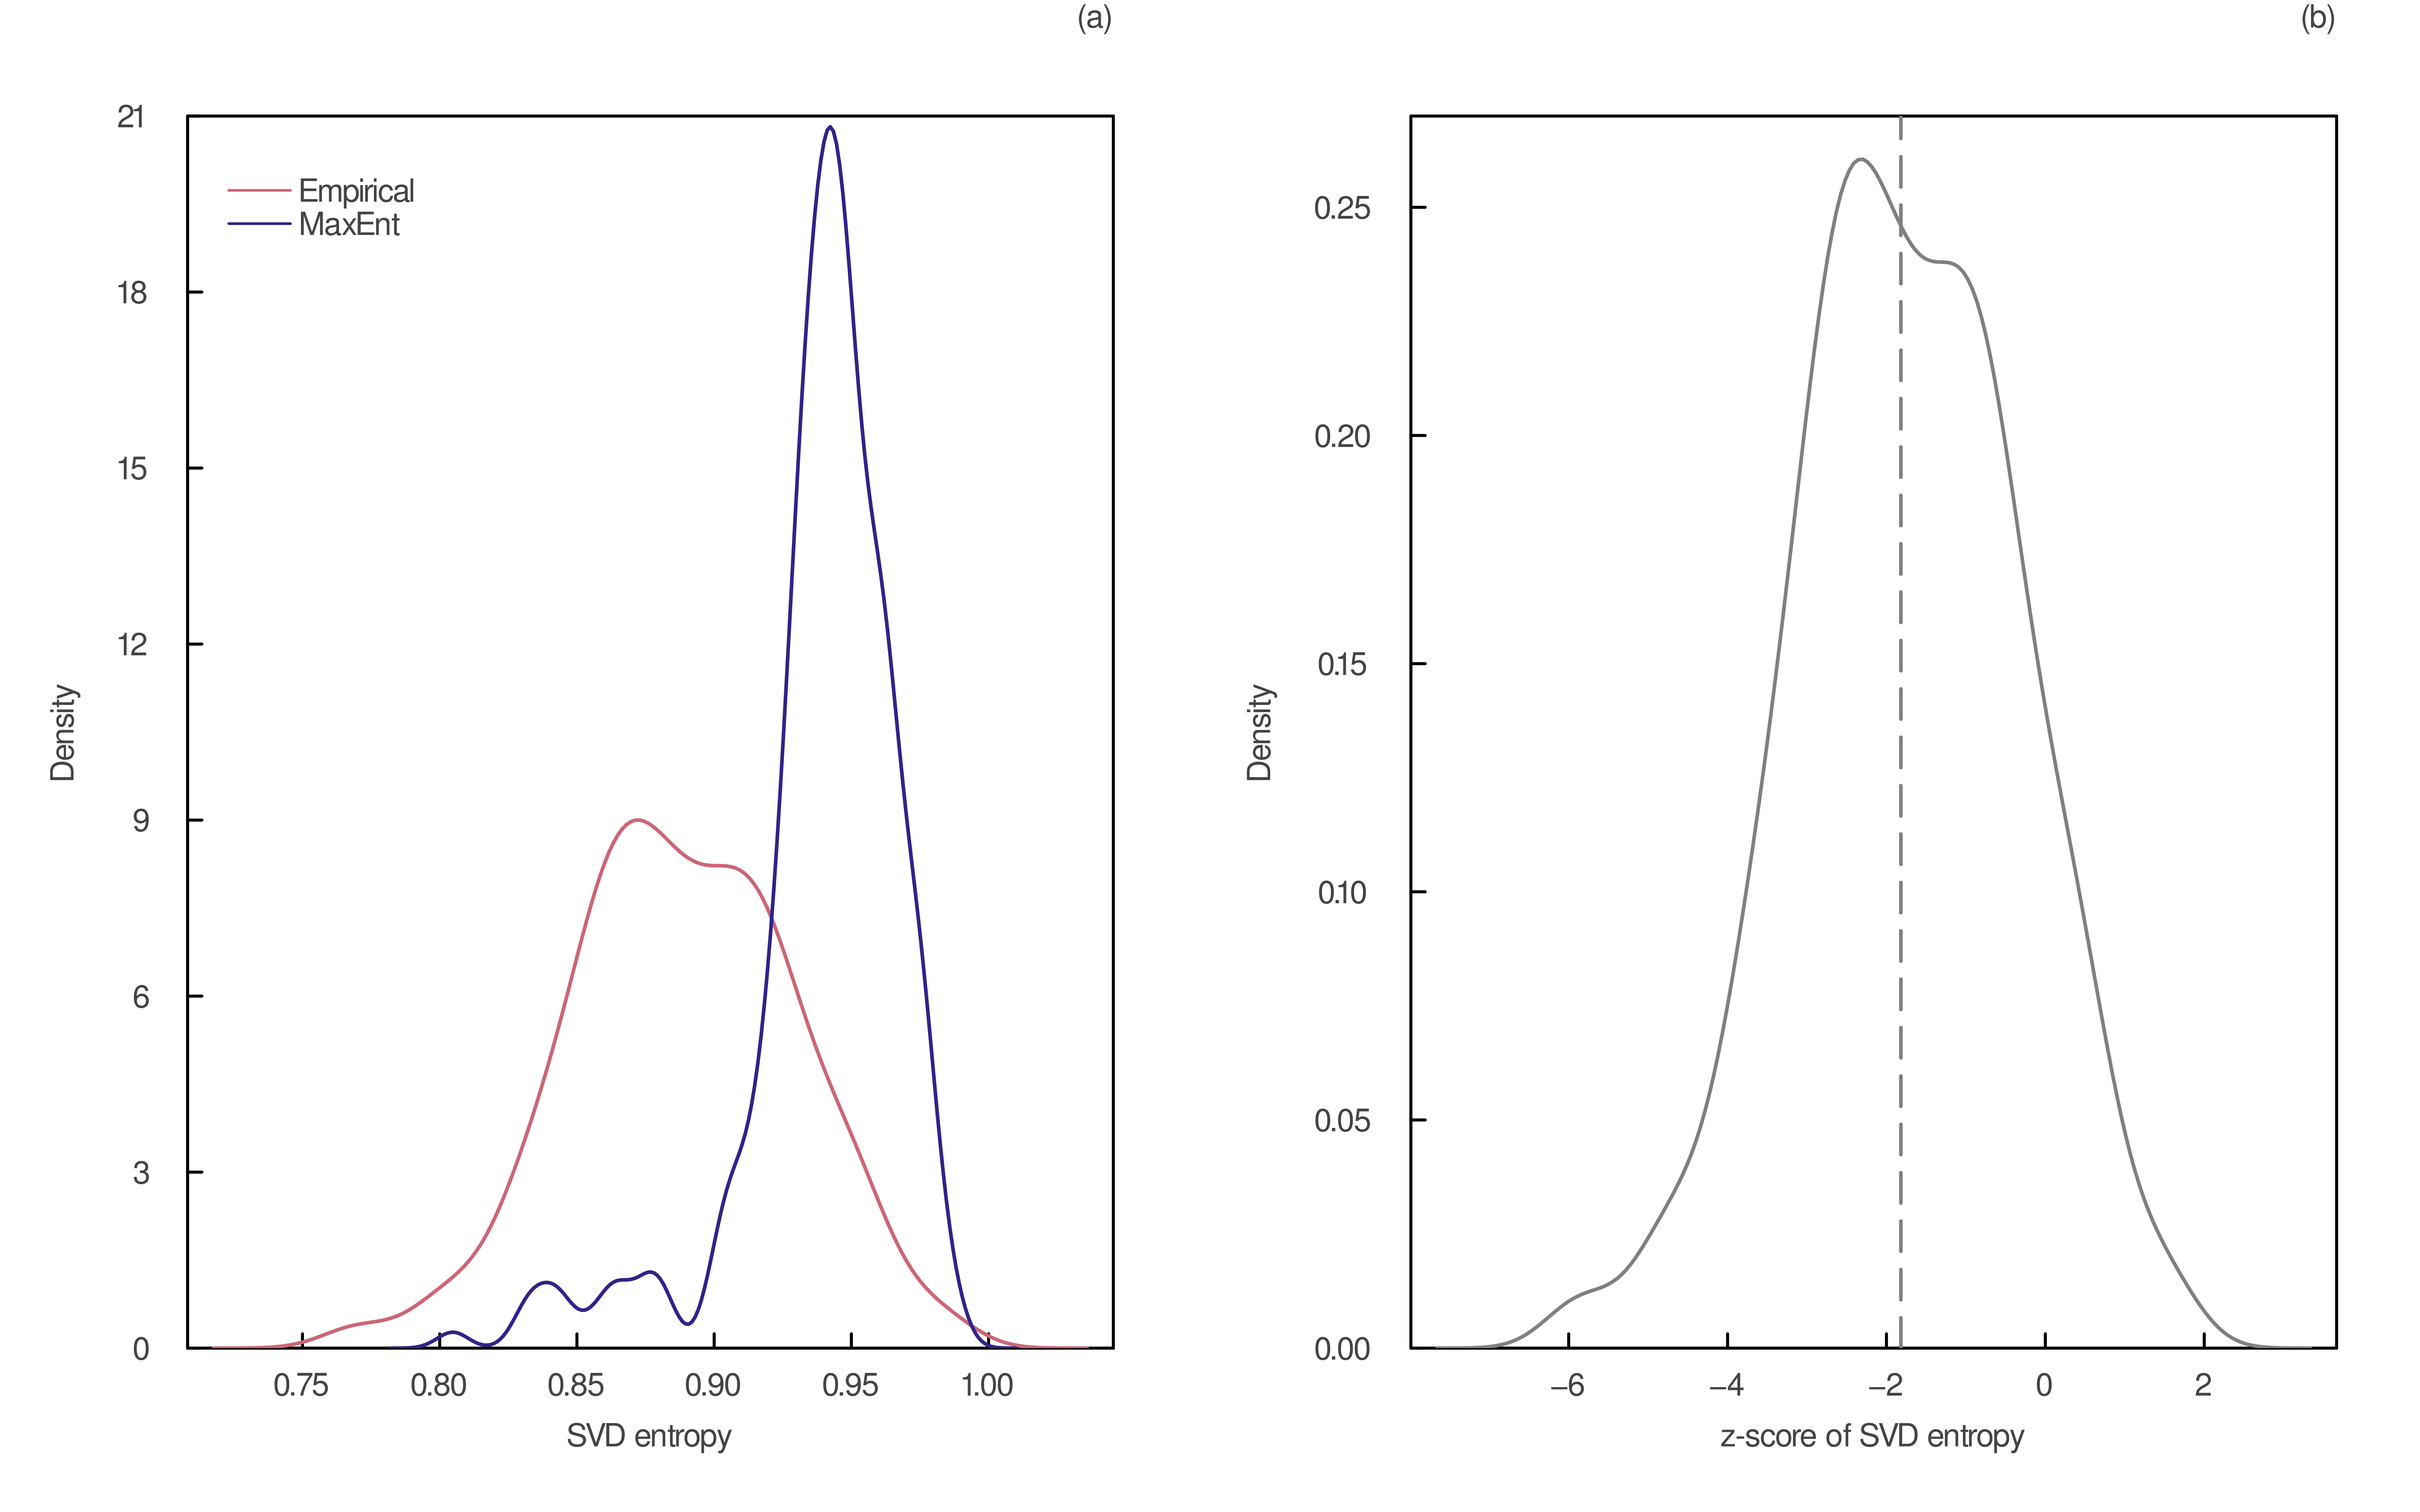
\includegraphics[width=\textwidth]{figures/S_article2/entropy_distribution.png}
    \caption{\textbf{SVD entropy of empirical and predicted food webs.} (a) Distribution of the
    SVD entropy of empirical and maximum entropy food webs. Maximum entropy networks
    were obtained using the type II heuristic MaxEnt model based on the joint degree
    sequence. (b) Distribution of z-scores of the SVD entropy of all empirical food
    webs. Z-scores were computed using the mean and standard deviation of the
    distribution of SVD entropy of MaxEnt food webs (type II heuristic MaxEnt
    model). The dashed line corresponds to the median
    z-score.}
    \label{fig:entropy_dist}
\end{figure}

\begin{figure}[h]
    \centering
    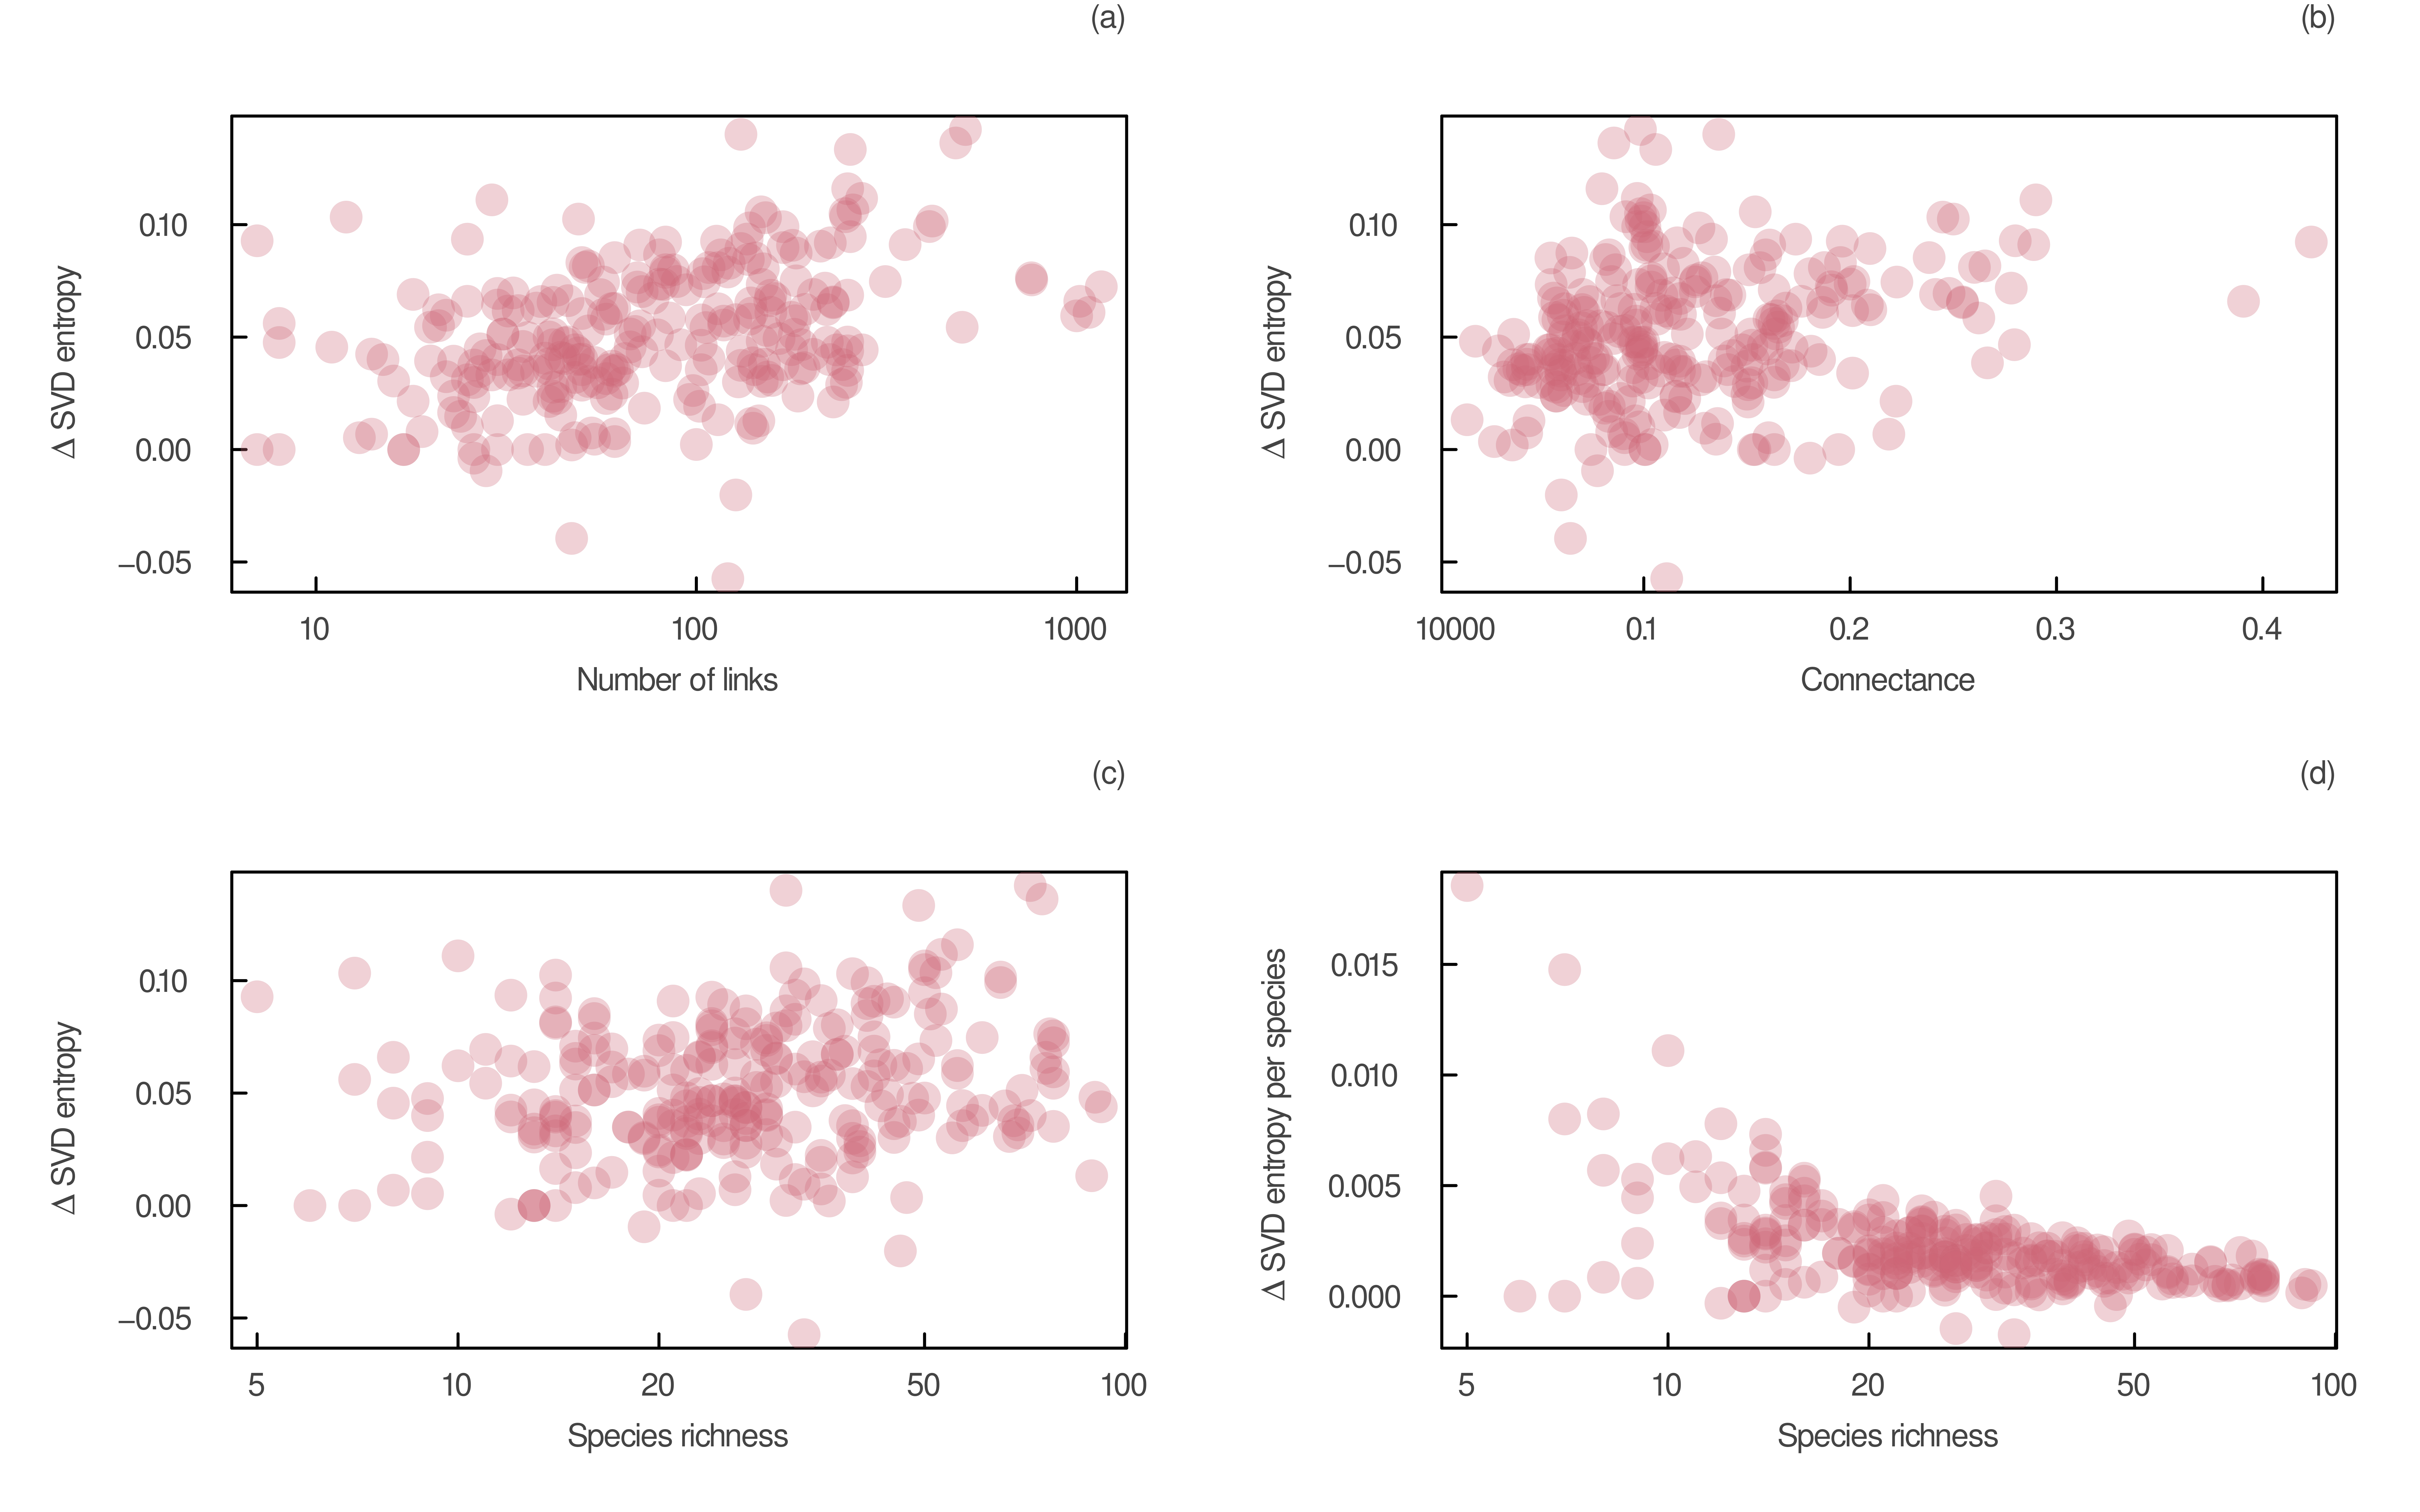
\includegraphics[width=\textwidth]{figures/S_article2/difference_entropy.png}
    \caption{\textbf{Prediction errors of SVD entropy.} Difference in SVD entropy between
    maximum entropy and empirical food webs as a function of (a) the number of
    interactions, (b) connectance, and (c) species richness. (d) Standardization of
    the difference in SVD entropy with respect to species richness as a function of
    species richness. The exponential decrease in the difference of SVD entropy per
    species with species richness offers a complementary perspective supporting the
    lack of relationship depicted in panel c. Maximum entropy networks were obtained
    using the type II heuristic MaxEnt model based on the joint degree
    sequence.}
    \label{fig:entropy_size}
\end{figure}

\begin{figure}[h]
    \centering
    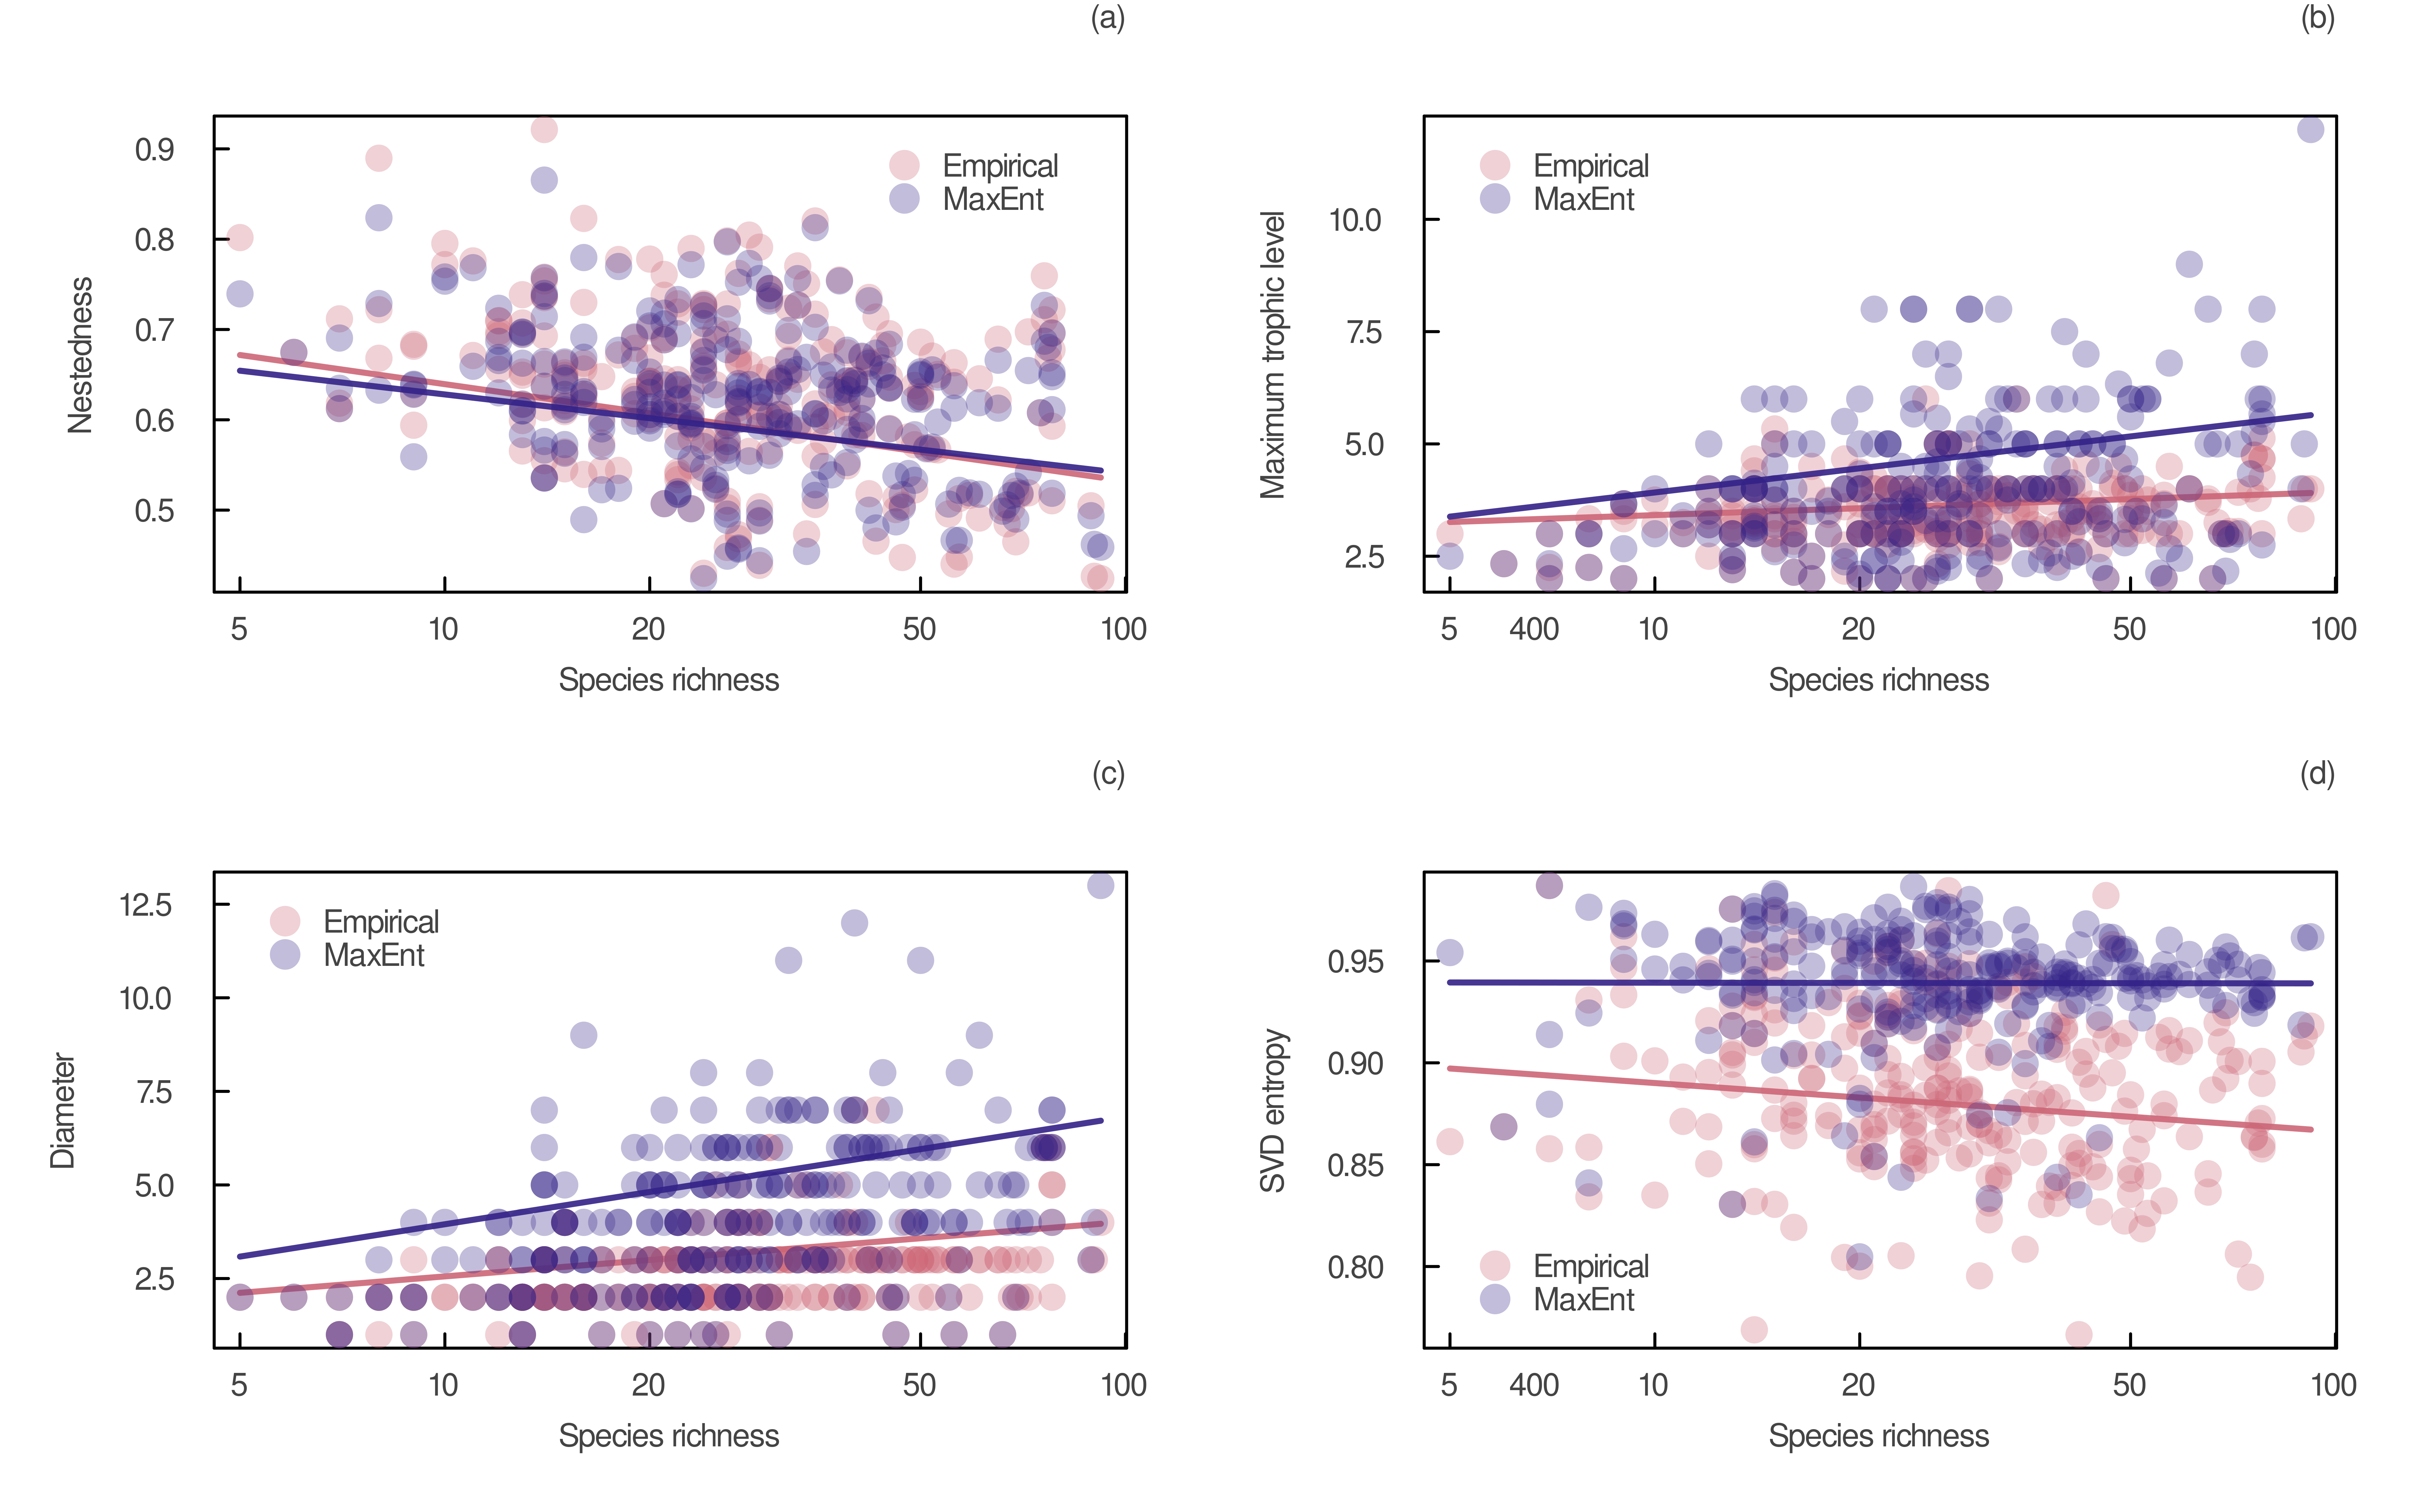
\includegraphics[width=\textwidth]{figures/S_article2/measures_richness.png}
    \caption{\textbf{Structure of empirical and maximum entropy food webs as a function of
    species richness.} Maximum entropy networks were obtained using the type II
    heuristic MaxEnt model based on the joint degree sequence. (a) Nestedness
    (estimated using the spectral radius of the adjacency matrix), (b) the maximum
    trophic level, (c) the network diameter, and (d) the SVD entropy were measured
    on these empirical and maximum entropy food webs and plotted against species
    richness. Regression lines are plotted in each
    panel.}
    \label{fig:measures_richness}
\end{figure}

\endinput
%%
%% End of file `S_article2.tex'.


\end{document}

\endinput
%%
%% End of file `phd_thesis.tex'.
